\batchmode
\makeatletter
\def\input@path{{lib}{styles/}{sections/}{pdf/}{chapters}}
\makeatother
\documentclass[ams,openany,10pt,presentation,latin1]{mathbook-main}
\usepackage{listings}
\usepackage{mathrsfs}
\graphicspath{{fig-pdf/}{pdf/}{image/}{sections/figures/}{figures/}{images/}}
\usepackage{float}
\usepackage{subfigure}
\definecolor{fondpaille}{cmyk}{0,0,0.1,0}
%\let\checkmark\relax
%\definecolor{bleu}{cmyk}{0.59,0.11,0,0.59}
%\definecolor{vert}{cmyk}{0.78,0,0.74,0.45}
%\definecolor{caper}{cmyk}{0.21,0.00,0.51,0.54}
%\definecolor{doc}{cmyk}{1.00,0.45,0.00,0.57}
%\definecolor{rhodo}{cmyk}{0.78,0,0.74,0.45}
%\definecolor{azulrey}{cmyk}{0.91,0.34,0.00,0.55}
%\definecolor{saddlebrown}{cmyk}{0.00,0.46,0.85,0.50}
%\definecolor{milktea}{cmyk}{0.00,0.18,0.43,0.22}
%\definecolor{naranja}{cmyk}{0,0.5,1,0}
%\definecolor{olivegreen}{cmyk}{0.64,0,0.95,0.40}
%\definecolor{bgpage}{cmyk}{.20,.30,.64,.19}
%\definecolor{mesh}{cmyk}{0,0.04,0.17,0.03}
\usepackage{pagecolor}
\usepackage{zahlen}
%\pagecolor{mesh}
\pagecolor{fondpaille}  
\lstset{
	numbers=left, 
	numberstyle=\tiny, 
	stepnumber=1, 
	numbersep=3pt, 
	language=[LaTeX]TeX, 
	backgroundcolor=\color{bleu!20},
	frame=shadowbox,
	rulesepcolor=\color{bleu},
	rulecolor=\color{bleu},
	framexleftmargin=10pt,
	keywordstyle=\color{vert}\bfseries,
	basicstyle=\listfont,
    columns=flexible,
    keepspaces=true,
    upquote=true,
    literate=
    {�}{{\'a}}{1}
    {�}{{\'e}}{1}
    {�}{{\'i}}{1}
    {�}{{\'o}}{1}
    {�}{{\'u}}{1}
    {�}{{\'A}}{1}
    {�}{{\'E}}{1}
    {�}{{\'I}}{1}
    {�}{{\'O}}{1}
    {�}{{\'U}}{1}
    {�}{{\~n}}{1}
    {�}{{\~N}}{1}
    {�}{{\"e}}{1}
    {�}{{\"U}}{1}%
    %frances
    {�}{{\`e}}{1}%
    {�}{{\`a}}{1}%
    {�}{{\^a}}{1}%%%
    {�}{{\c{c}}}{1}%
    {?}{{\oe}}{1}%
    {�}{{\`u}}{1}%
    {�}{{\`E}}{1}%
    {�}{{\`A}}{1}%
    {�}{{\c{C}}}{1}%
    {?}{{\OE}}{1}%
    {�}{{\^E}}{1}%
    {�}{{\^e}}{1}%
    {�}{{\^i}}{1}%
    {�}{{\"i}}{1}%%%
    {�}{{\^o}}{1}%
    {�}{{\^u}}{1}%
    ,
    commentstyle=\color{gray},
    morekeywords={redefineColor,dfrac,setlength,cellspacetoplimit, cellspacebottomlimit,firstline,text,intro,introauthor,chapter, itemclass,exostart,corrstart,PagCorregidos,columnbreak,titlepic, nbcolindex,indexname,printindex,makeindex,activites, DefineNewBoxLikeRem,BreakCorr}
}
\usepackage{lipsum-es}
\usepackage{wasysym}
\makeatletter 
\newenvironment{proof}[1][Prueba]{\textcolor{dem@line@color}{\textbf{#1.\phantom{--}} }}{\hfill\phantom{--}\hfill\ \ \textcolor{dem@line@color}{\rule{0.5em}{0.5em}}}
\newenvironment{exam}[1][Ejercicio]{\textbf{#1.}\ }{\hfill\ \rule{0.5em}{0.5em}}
\newenvironment{sol}[1][Soluci\'on]{\textcolor{dem@line@color}{\textbf{#1.\phantom{--}}}}{\hfill\phantom{--}\hfill\ \textcolor{dem@line@color}{\checked}}

\RequirePackage[colorlinks=true,linkcolor=corref@color]{hyperref}
\redefineColor{thmtitle@bg@color}{0.66,0.24,0.74,0.71}
\redefineColor{thm@bg@color}{0.11,0,0.09,0.09}
\redefineColor{proptitle@bg@color}{0.66,0.24,0.74,0.71}
\redefineColor{prop@bg@color}{0.11,0,0.09,0.09}
\redefineColor{firstpagebottom@bg@color}{1,1,0.00,0.55}
\redefineColor{subsection@title@color}{.19,.74,.100,.68}
%%%%%%%%%%%%%%%%%%%%%%%%%%%%%%%%%%%%%%%%%%%%%%%%%%%%%%%%%%%%%%%%%%
\def\Vdots{\vbox{\baselineskip4\p@ \lineskiplimit\z@
    \kern6\p@\hbox{.}\hbox{.}\hbox{.}}}
%%%%%%%%%%%%%%%%%%%%%%%%%%%%%%%%%%%%%%%%%%%%%%%%%%%%%%%%%%%
\makeatother
%\selectspanish
\title{C\'alculo diferencial\\ \normalsize Con ejercicios resueltos.}
\author{Antalcides Olivo}
\titlepic[0.3]{image/puente1.jpg}
\logopic[1]{image/logo-caos-1.png}
%\titlepic[0.5]{fractal.jpg}
\date{\dia}

\makeindex
%\usepackage[mathrm=sym]{unicode-math}
%\setmathfont{Fira Math Regular}
%\DeclareMathAlphabet{\mathcal}{OMS}{cmbrs}{m}{n}
\defaultfontfeatures[FiraMath-Regular.otf]
    { Path = {C:/texlive/texmf-local/fonts/opentype/public/firamath/} ,
      Extension = .otf }
 \begin{document}

\frontmatter

\maketitle

{
\makeatletter
\sectiontitle@font
\tableofcontents
\makeatother
}

\mainmatter

\intro{Nada se pierde, todo se transforma}
\introauthor{Lavoisier}
%%------------------------------------------------------------------------
%%% Cap�tulo paquetes
%%------------------------------------------------------------------------
AAAA \\bbb
%

\pagecolor{fondpaille}  
\chapter{Funciones reales de variable real}

\section{Introducci\'{o}n}

Este curso es sobre C\'{a}lculo diferencial de funciones reales de variable
real. En ese sentido, los objetos sobre los cuales se trabajar\'{a} son
funciones definidas en subconjuntos del conjunto de los n\'{u}meros reales y
con valores o \textquotedblleft im\'{a}genes\textquotedblright\ reales. En
este primer cap\'{\i}tulo se presentan los principales t\'{o}picos relativos a
dichas funciones y los cuales son importantes para el desarrollo mismo del
curso. Algunas de las definiciones que se presentan son tambi\'{e}n
v\'{a}lidas para funciones en general.

\paragraph{}

Prerrequisitos importantes para el curso son:

\begin{enumerate}
\item El Algebra de reales. Es decir, el conocimiento y manejo b\'{a}sico de
la estructura de campo $(\rz,+,\cdot)$, constituida por el conjunto de los
n\'{u}meros reales, $\rz$, con las operaciones de adici\'{o}n y
multiplicaci\'{o}n. Otras propiedades, topol\'{o}gicas (geom\'{e}tricas),
necesarias se introducen en el siguiente cap\'{\i}tulo.

\item Trigonometr\'{\i}a b\'{a}sica. En particular, manejo de las razones
trigonom\'{e}tricas para \'{a}ngulos cualesquiera y las identidades fundamentales.
\end{enumerate}

Se supone un conocimiento de tales t\'{o}picos gracias a un curso previo de
Algebra y Trigonometr\'{\i}a. Para consultas sobre estos temas se recomiendan
\cite{Taylor}, \cite{Vance} y \cite{leh}, especialmente. Tambi\'{e}n textos de
m\'{a}s reciente edici\'{o}n como \cite{Lei} y \cite{Swo} pueden ser de utilidad.

\paragraph{}

Utilizaremos las siguientes notaciones para los subconjuntos notables del
conjunto de los n\'{u}meros reales:
\begin{align*}
\nz  &  =\gz^{+}\\
&  =\{1,2,3,\dots\}\ \mbox{(Naturales, Enteros positivos)}\\
\nz_{0}  &  =\gz_{+}\\
&  =\{0,1,2,\dots\}\ \mbox{(Cardinales, Enteros no negativos)}\\
\gz  &  =\{\dots,-3,-2,-1,0,1,2,3,\dots\}\ \mbox{(Enteros)}\\
\gz^{-}  &  =\{\dots,-3,-2,-1\}\ \mbox{(Enteros negativos)}\\
\qz  &  =\left\{  \left.  \frac{a}{b}\ \right\vert \ a,b\in\gz,b\neq0\right\}
\ \mbox{(Racionales)}
\end{align*}
$\qz^{\prime}$ denotar\'{a} al conjunto de los n\'{u}meros irracionales.
%\nopagebreak{4}
%\pagebreak


\section{Definiciones b\'{a}sicas}

Dados conjuntos no vac\'{\i}os $A$ y $B$, el producto cartesiano
\index{Producto cartesiano|textbf}
de $A$ por $B$ es el conjunto
\begin{equation}
A\times B=\{(a,b)\mid a\in A,b\in B\}
\end{equation}
Un elemento $(a,b)$ de $A\times B$ es denominado un par ordenado. El
car\'{a}cter de \textquotedblleft ordenado\textquotedblright\ viene dado por
la definici\'{o}n siguiente para elementos $a,c\in A$ y $b,d\in B$:
\[
(a,b)=(c,d)\Longleftrightarrow a=c\wedge b=d
\]
que establece as\'{\i} que el orden de las \textquotedblleft
componentes\textquotedblright\ del par es importante.

\paragraph{}

Una
\index{Relaci\'{o}n|textbf}
relaci\'{o}n del conjunto $A$ al conjunto $B$ es un subconjunto cualquiera no
vac\'{\i}o del producto cartesiano $A\times B$. Si $R$ es una relaci\'{o}n y
$(a,b)\in R$ decimos que $b$ es una im\'{a}gen de $a$ bajo $R$.

\begin{example}
\label{ejemplouno} As\'{\i}, por ejemplo, si $A=\{a,b,c\},B=\{0,1,2,3\}$, los
si\-guientes conjuntos son relaciones de $A$ a $B$:
\begin{align*}
K  &  =\{(a,0),(b,0),(a,1),(b,2)\}\\
S  &  =\{(a,0),(b,1),(c,2),(a,3)\}\\
T  &  =A\times B\\
F  &  =\{(a,0),(b,2),(c,1)\}\\
G  &  =\{(a,1),(b,2),(c,3)\}
\end{align*}

\end{example}

\paragraph{}

Para una relaci\'{o}n $R$ de $A$ a $B$, el subconjunto de $A$ formado por las
primeras componentes de $R$ es denominado%
\index{Dominio|textbf}
dominio de la relaci\'{o}n $R$ y se nota $\operatorname*{Dom}(R)$. El conjunto
de las segundas componentes, subconjunto de $B$, se denomina rango%
\index{Rango|textbf}
de $R$ y se nota $\operatorname*{Ran}(R)$. Es claro que un elemento del
dominio de una relaci\'{o}n puede tener m\'{a}s de una im\'{a}gen. En el
ejemplo \ref{ejemplouno} se tienen:%

\[%
\begin{tabular}
[c]{lll}%
$\operatorname*{Dom}(K)=\{a,b\}$ &  & $\operatorname*{Ran}(K)=\{0,1,2\}$\\
$\operatorname*{Dom}(S)=\{a,b,c\}=A$ &  & $\operatorname*{Ran}%
(S)=\{0,1,2,3\}=B$\\
$\operatorname*{Dom}(T)=A$ &  & $\operatorname*{Ran}(T)=B$\\
$\operatorname*{Dom}(F)=\{a,b,c\}$ &  & $\operatorname*{Ran}(F)=\{0,1,2\}$\\
$\operatorname*{Dom}(G)=A$ &  & $\operatorname*{Ran}(G)=\{1,2,3\}$%
\end{tabular}
\ \ \
\]
N\'{o}tese que en $F$ y $G$ el dominio es $A$ y que cada elemento del dominio
tiene una im\'{a}gen \'{u}nica. Una relaci\'{o}n $R$ de $A$ a $B$ es
denominada una%
\index{Funci\'{o}n|textbf}
funci\'{o}n si $\operatorname*{Dom}(R)=A$ y cada elemento del dominio tiene
una im\'{a}gen \'{u}nica. Es decir, no existen dos pares ordenados distintos
con la misma primera componente. Por lo tanto, $F$ y $G$ son las \'{u}nicas
funciones de $A$ a $B$ en el ejemplo conside\-rado. En lo que sigue
utilizaremos letras como $f,g,$ etc o letras griegas ($\varphi,\psi,$ etc)
para denotar funciones. Si $f$ es una funci\'{o}n de $A$ a $B$ y $x\in A$,
denotaremos por $f(x)$ a la
\index{Imagen|textbf}%
im\'{a}gen (\'{u}nica) de $x$ bajo $f$. Se acostumbra tambi\'{e}n a escribir
\[
f:A\longrightarrow B
\]
para referirse a una funci\'{o}n $f$ cuyo dominio es el conjunto $A$ y cuyo
conjunto de llegada, o recorrido, es $B$.

\paragraph{}

A menudo es muy \'{u}til ver una funci\'{o}n como una transformaci\'{o}n, en
el sentido de que toma cada elemento del dominio, $A$, y lo transforma en un
elemento del conjunto $B$. El esquema siguiente ilustra tal situaci\'{o}n. En
el mismo consideramos a $f$ como una \textquotedblleft
m\'{a}quina\textquotedblright\ que toma su materia prima del dominio y produce
o arroja resultados (las im\'{a}genes) en el conjunto de llegada.
\[
A\ni x\longrightarrow\framebox[2cm]{$f$}\longmapsto f(x)\in B.
\]
Tambi\'{e}n es usual el esquema
\[%
\begin{tabular}
[c]{cccc}%
$f:$ & $A$ & $\longrightarrow$ & $B$\\
& $x$ & $\longmapsto$ & $f(x)$%
\end{tabular}
\ \ \
\]


%$$\matrix{f:&A&\longrightarrow &B\cr &x&\longmapsto& f(x)}$$


N\'{o}tese que si $f:A\longrightarrow B,g:A\longrightarrow B$ , entonces
\begin{equation}
f=g\ \Longleftrightarrow\ f(x)=g(x)\ \mbox{ \ para todo \ }x\in A.
\label{igualdadfunciones}%
\end{equation}


\paragraph{}

La funci\'{o}n $f:A\longrightarrow B$ se denomina
\index{Funci\'{o}n!-- sobreyectiva}%
sobreyectiva, o simplemente sobre, si se cumple que $\operatorname*{Ran}%
(f)=B$. $f$ se
\index{Funci\'{o}n!-- inyectiva}%
denomina inyectiva o uno-a-uno si cada elemento del rango es im\'{a}gen de un
\'{u}nico elemento del dominio. Se tiene as\'{\i}:

\begin{description}
\item[i.] $f:A\longrightarrow B$ es sobre si, y solo si para todo $y\in B$,
existe $x\in A$ tal que $y=f(x).$

\item[ii.] $f:A\longrightarrow B$ es uno-a-uno si, y solo si para todo $x,u\in
A$ se cumple que
\[
f(x)=f(u)\Longrightarrow x=u
\]

\end{description}

La segunda proposici\'{o}n es equivalente a :

\begin{quotation}
\noindent$f:A\longrightarrow B$ \ es \ uno-a-uno \ si, y solo si \ para todo
$y\in\operatorname*{Ran}(f)$ la ecuaci\'{o}n (en $x$) $f(x)=y$ tiene
soluci\'{o}n \'{u}nica.
\end{quotation}

Nuestro objeto de estudio son funciones%
\index{Funci\'{o}n!-- de valor real}
reales de variable real. Una tal funci\'{o}n es una funci\'{o}n de la forma
\[
f:A\longrightarrow\rz,
\]
donde $A$ es un subconjunto cualquiera de $\rz$. En general, la
\textquotedblleft naturaleza\textquotedblright\ de la variable la da el
dominio de la funci\'{o}n y la de la funci\'{o}n la da el rango o el conjunto
de llegada. As\'{\i}, al hablar de funciones reales de variable real queremos
indicar que la funci\'{o}n transforma reales en reales. Son tales funciones
las que consideraremos en este curso.

Es muy com\'{u}n definir una funci\'{o}n como las consideradas indicando la
manera como las im\'{a}genes se obtienen a partir de los elementos del
dominio, sin indicar espec\'{\i}ficamente \'{e}ste \'{u}ltimo, el cu\'{a}l en
todo caso es un subconjunto de los reales. En tales casos, el dominio se
entender\'{a} como el mayor subconjunto posible de los reales para el cual las
im\'{a}genes est\'{a}n definidas; es decir, para el cual las im\'{a}genes son
n\'{u}meros reales.

\begin{example}
Consid\'{e}rese, por ejemplo, la funci\'{o}n $f$ tal que para un $x$
cualquiera en su dominio se tiene
\[
f(x)=\sqrt{x^{2}+3x+2}.
\]
En este caso, el dominio de $f$ es el conjunto de todas los reales $x$ para
los cuales
\[
x^{2}+3x+2\geq0.
\]
Resolviendo la inecuaci\'{o}n anterior se obtiene
\begin{align*}
&  x^{2}+3x+2\geq0\\
\Longleftrightarrow &  (x+2)(x+1)\geq0\\
\Longleftrightarrow &  x\leq-2\vee x\geq-1\\
\Longleftrightarrow &  x\in\left]  -\infty,-2\right]  \cup\left[
-1,+\infty\right[
\end{align*}
As\'{\i}, se tiene entonces $\operatorname*{Dom}(f)=\left]  -\infty,-2\right]
\cup\left[  -1,+\infty\right[  $\footnote{Esta notaci\'{o}n se acostumbra a
utilizar para evitar confusiones con el \textquotedblleft par ordenado"
$(a,b)$.}. Para la funci\'{o}n $g$ definida por $g(x)=\dfrac{x+3}{x^{2}%
-5x-6},$ se tiene
\begin{align*}
g(x)\in\rz &  \Longleftrightarrow x^{2}-5x-6\neq0\\
&  \Longleftrightarrow(x-6)(x+1)\neq0\\
&  \Longleftrightarrow x\neq6\wedge x\neq-1,
\end{align*}
de donde se obtiene que $\operatorname*{Dom}(g)=\rz-\{-1,6\}$.
\end{example}

\paragraph{}

Dada una funci\'{o}n $f:A\longrightarrow B$, si $C$ es un subconjunto no
vac\'{\i}o de $A$, la restricci\'{o}n de%
\index{Funci\'{o}n!Restricci\'{o}n de una --}
$f$ a $C$, es la funci\'{o}n $f|_{C}$, definida por
\begin{equation}
f|_{C}(x)=f(x),\ \mbox{ \ para todo \ }x\in C. \label{restriccion}%
\end{equation}
As\'{\i}, sobre $C$, $f$ coincide con su restricci\'{o}n. Se acostumbra
tambi\'{e}n decir que $f$ es una extensi\'{o}n de $f|_{C}$.

\section{Gr\'{a}ficas de funciones reales de variable real}%

\index{Relaci\'{o}n!Gr\'{a}fica de una --}%
Notaremos mediante $\rz^{2}$ al conjunto de todos los pares ordenados de
n\'{u}meros reales. Es decir:
\[
\rz^{2}=\rz\times\rz=\{(x,y)\mid x,y\in\rz\}.
\]
Cada par de reales puede identificarse con un punto del plano euclidiano,
introduciendo un sistema rectangular de coordenadas en el mismo. Fijado el
sistema de coordenadas, la correspondencia entre puntos del plano y pares
ordenados de reales es biun\'{\i}voca. Dado un par ordenado $(x,y)$, el mismo
puede representarse como el punto del plano cuyas distancias dirigidas
(coordenadas) a los ejes de coordenadas ($X$ e $Y$) son $y$ y $x$,
respectivamente, como seguramente conoce el lector. La notaci\'{o}n $P(x,y)$
se referir\'{a} a un punto $P$ del plano cuyas coordenadas cartesianas son $x$
e $y$. En tal sentido, una relaci\'{o}n real (esto es, un subconjunto de
$\rz^{2}$) puede representarse como un subconjunto de puntos del plano, al
cual denominaremos la gr\'{a}fica de la relaci\'{o}n. As\'{\i}, si $R$ es una
relaci\'{o}n real, tenemos que la gr\'{a}fica de $R$ es el conjunto
\[
\operatorname*{graph}(R)=\{P(x,y)\mid(x,y)\in R\}.
\]%
\index{Funci\'{o}n!Gr\'{a}fica de una --}%
Algunas funciones notables y sus gr\'{a}ficas se presentan a continuaci\'{o}n,

\begin{example}{\bf La funci\'{o}n lineal:\ }%
\index{Funci\'{o}n!-- lineal}%
Si $a$ y $b$ son reales cualesquiera, la funci\'{o}n definida por
\begin{equation}
f(x)=ax+b,\mbox{ \ para todo real \ }x, \label{deffuncionlineal}%
\end{equation}
se denomina funci\'{o}n lineal. Si $a\neq0$, la ecuaci\'{o}n (lineal) en $x$
\[
ax+b=y
\]
tiene soluci\'{o}n \'{u}nica para todo $y\in\rz$. Se tiene entonces que $f$ es
biyectiva (uno-a-uno y sobre) y su gr\'{a}fica es una recta con pendiente
distinta de cero (no es paralela al eje $x$). Si $a=0$, se tiene la
funci\'{o}n constante definida por $f(x)=b$, cuya gr\'{a}fica es una recta
paralela al eje $x$ (ver figuras \ref{flineal} ).
\end{example}

%TODO

\begin{figure}[H]
\centering
\includegraphics[scale=0.6]%
{../mathbook-caos-calculo/images/ej-1-3-1.pdf}%
\caption{Funci\'{o}n lineal}%
\label{flineal}%
\end{figure}



Un caso particular importante de la funci\'{o}n lineal es la funci\'{o}n
identidad definida por
\begin{equation}
I_{\rz}(x)=x \label{funcionidentidad}%
\end{equation}
que se obtiene para $a=1$, $b=0$ en (\ref{deffuncionlineal}).

\begin{example}{\bf Funci\'{o}n cuadr\'{a}tica:}
\index{Funci\'{o}n!-- cuadr\'{a}tica}%
Una funci\'{o}n definida por una expresi\'{o}n de la forma
\[
f(x)=ax^{2}+bx+c,
\]
donde $a,b,c$ son reales con $a\neq0$, es denominada funci\'{o}n
cuadr\'{a}tica. Es claro que $\operatorname*{Dom}(f)=\rz$. Para determinar el
rango, consideramos la ecuaci\'{o}n cuadr\'{a}tica (en $x$)%
\[
ax^{2}+bx+c-y=0.
\]
Tal ecuaci\'{o}n tiene soluciones reales si, y solo si
\[
b^{2}-4a(c-y)\geq0\Longleftrightarrow4ay\geq4ac-b^{2}%
\]
Tenemos entonces:

\begin{enumerate}
\item Si $a>0$, entonces $y\geq\frac{4ac-b^{2}}{4a}$. La funci\'{o}n tiene
as\'{\i} un valor m\'{\i}nimo $\frac{4ac-b^{2}}{4a}$. Su rango es el conjunto
\[
\left[  \left.  \frac{4ac-b^{2}}{4a},+\infty\right.  \right[  .
\]


\item Si $a<0$, entonces $y\leq\frac{4ac-b^{2}}{4a}$. $f$ tiene un valor
m\'{a}ximo $\frac{4ac-b^{2}}{4a}$ y su rango es%
\[
\left]  -\infty,\left.  \frac{4ac-b^{2}}{4a}\right.  \right]
\]

\end{enumerate}

En ambos casos el valor m\'{a}ximo o m\'{\i}nimo se alcanza para
$y=\frac{4ac-b^{2}}{4a}$, es decir para $x=\frac{-b}{2a}$. El punto $V\left(
\frac{-b}{2a},\frac{4ac-b^{2}}{4a}\right)  $ es denominado V\'{e}rtice de la
gr\'{a}fica de $f$ y corresponde al punto \textquotedblleft m\'{a}s
bajo\textquotedblright\ o \textquotedblleft m\'{a}s alto\textquotedblright\ de
la gr\'{a}fica.

N\'{o}tese que la gr\'{a}fica de $f$ es la gr\'{a}fica de la ecuaci\'{o}n en
dos variables $y=ax^{2}+bx+c$, la cual puede escribirse como
\begin{equation}
y-\frac{4ac-b^{2}}{4a}=\left(  x-\frac{-b}{2a}\right)  ^{2}%
\end{equation}

\end{example}

As\'{\i}, si $x\neq\frac{-b}{2a}$, entonces para cada valor de $y$ en el rango
de $f$, existen dos valores de $x$ de los cuales $y$ es im\'{a}gen, a saber:
\[
x=\frac{-b}{2a}\pm\sqrt{y-\frac{4ac-b^{2}}{4a}}%
\]
lo cual muestra que la gr\'{a}fica de $f$ es sim\'{e}trica con relaci\'{o}n a
la recta de ecuaci\'{o}n $x=\frac{-b}{2a}$. Tal recta es denominada eje de
simetr\'{\i}a de la gr\'{a}fica de $f$. La gr\'{a}fica es una par\'{a}bola%
\index{Par\'{a}bola|textbf}
que \textquotedblleft abre\textquotedblright\ hacia arriba si $a>0$, y hacia
abajo si $a<0$ (ver figuras \ref{parabolas}).%



\begin{figure}[H]
\centering
\includegraphics[scale=0.5]%
{../mathbook-caos-calculo/images/ej-1-3-2.pdf}%
\caption{Funci\'{o}n Cuadr\'{a}tica}%
\label{parabolas}%
\end{figure}



\section*{Funciones definidas impl\'{\i}citamente}

Si $F:A\longrightarrow\rz$ es una funci\'{o}n real, con $A\subseteq\rz^{2}$,
entonces el dominio de $F$ es un conjunto de pares ordenados de reales. Una
tal funci\'{o}n es denominada una
\index{Funci\'{o}n!-- definida implicitamente}%
funci\'{o}n real en dos variables. Para $(x,y)\in A$, escribiremos, por
comodidad, $F(x,y)$, en lugar de $F((x,y))$, para referirnos a la im\'{a}gen
del par $(x,y)$ bajo la funci\'{o}n $F$. Para un real $b$ la ecuaci\'{o}n
$F(x,y)=b$ es una ecuaci\'{o}n en las variables $x,y$. Cada soluci\'{o}n de
dicha ecuaci\'{o}n, si las tiene, es un par ordenado $(u,v)$, en el dominio de
$F$, tal que la proposici\'{o}n
\[
F(u,v)=b
\]
es verdadera. Es decir, la ecuaci\'{o}n se satisface para el par de valores
$x=u,y=v$. Los ejemplos de la funci\'{o}n lineal y la funci\'{o}n
cuadr\'{a}tica muestran casos particulares de funciones reales de variable
real definidas por ecuaciones en las variables $x,y$. As\'{\i}, por ejemplo,
la funci\'{o}n lineal dada por $f(x)=2x+3$ puede definirse como el conjunto de
las soluciones de la ecuaci\'{o}n $y=2x+3$ o $y-2x=3$. Es decir, podemos
escribir
\[
f=\{(x,y)\in\rz^{2}\mid y-2x=3\}.
\]
En general, decimos que una funci\'{o}n $f$ est\'{a} definida
impl\'{\i}citamente por la ecuaci\'{o}n $F(x,y)=b$ si para todo $u\in
\operatorname*{Dom}(f)$, el par $(u,f(u))$ es soluci\'{o}n de la ecuaci\'{o}n
dada; es decir si se cumple que $F(u,f(u))=b$ es una proposici\'{o}n
verdadera. En otras palabras, la funci\'{o}n (como conjunto de pares
ordenados) est\'{a} contenida en el conjunto soluci\'{o}n de la ecuaci\'{o}n.
Sin embargo, el conjunto soluci\'{o}n de la ecuaci\'{o}n $F(x,y)=b$ no
necesariamente constituye una funci\'{o}n real de variable real, aunque
s\'{\i} es claro que es una relaci\'{o}n real.

Consideremos, por ejemplo, la ecuaci\'{o}n en dos variables $x^{2}+y^{2}=1$,
cuya gr\'{a}fica, como seguramente lo sabe el lector, es una circunferencia
con centro en el origen y radio $1$. Es claro que el conjunto soluci\'{o}n de
tal ecuaci\'{o}n- es decir, el conjunto cuya gr\'{a}fica es la circunferencia-
no es una funci\'{o}n ya que un mismo elemento del dominio (p.e, $x=0$) puede
tener m\'{a}s de una im\'{a}gen ($1$ y $-1$, en el caso indicado). Sin
embargo, cualquiera de las funciones definidas a continuaci\'{o}n est\'{a}
impl\'{\i}citamente definida por la ecuaci\'{o}n dada.

\begin{enumerate}
\item $y=f(x)=\sqrt{1-x^{2}}$.

\item $y=g(x)=-\sqrt{1-x^{2}}$.

\item
\[
y=h(x)=%
\begin{cases}
\sqrt{1-x^{2}}, & \text{si $-1\leq x\leq0$}\\
-\sqrt{1-x^{2}}, & \text{ si $0<x\leq1$}%
\end{cases}
\]

\end{enumerate}

\section{Algebra de funciones}%

\index{Funciones!Algebra de --}%
Dado que el conjunto de los n\'{u}meros reales est\'{a} dotado de una
estructura aditivo-multiplicativa, las im\'{a}genes bajo funciones reales
pueden sumarse y multiplicarse, as\'{\i} como restarse y dividirse, si dicha
divisi\'{o}n est\'{a} definida. Esto permite definir operaciones algebraicas
entre funciones con valores reales.

\begin{definition}
Sean $A$ y $B$ conjuntos tales que $A\cap B\neq\emptyset$ y
\[
f:A\longrightarrow\rz,g:B\longrightarrow\rz
\]
funciones reales. Definimos para $x\in A\cap B$:
\begin{align}
(f+g)(x)  &  =f(x)+g(x)\label{sumafuncion}\\
(fg)(x)  &  =f(x)g(x) \label{productofuncion}%
\end{align}

\end{definition}

Las funciones $f+g$ y $fg$ definidas en (\ref{sumafuncion}) y
(\ref{productofuncion}) son, respectivamente, las funciones
\index{Funciones!Suma de --}%
suma y producto%
\index{Funciones!Producto de --}
de $f$ y $g$. Rigurosamente hablando, las funciones sumadas o multiplicadas
son las restricciones de $f$ y $g$ a la intersecci\'{o}n de sus dominios. Por
supuesto, podemos tambi\'{e}n definir funciones
\index{Dominio!-- de la funci\'{o}n producto.}%
\index{Dominio!-- de la funci\'{o}n cociente}
diferencia%
\index{Dominio!-- de la funci\'{o}n suma}
($f-g$) y cociente ($f/g$), esta \'{u}ltima en el conjunto de todos los $x\in
A\cap B$ para los cuales $g(x)\neq0$.

En particular, la suma de una funci\'{o}n real con una funci\'{o}n constante
constituye, geom\'{e}tricamente hablando, una traslaci\'{o}n de la gr\'{a}fica%
\index{Funci\'{o}n!Gr\'{a}fica de una --!Traslaci\'{o}n|textit}
de $f$ con relaci\'{o}n al eje $Y$. La figura \ref{traslacionejey1} ilustra la
situaci\'{o}n: la gr\'{a}fica de $f+g$, siendo $g(x)=k$, para una constante
$k$ (positiva en el ejemplo mostrado), es un desplazamiento vertical de la
gr\'{a}fica de $f$.%


\begin{figure}[H]
\centering
\includegraphics[scale=0.6]
{../mathbook-caos-calculo/images/ej-1-3-3.pdf}%
\caption{Suma de una funci\'{o}n con una constante}%
\label{traslacionejey1}%
\end{figure}


Por su parte, el producto de una funci\'{o}n real $f$ por una funci\'{o}n
constante positiva y diferente de $1$ produce una
\index{Funci\'{o}n!Gr\'{a}fica de una --!Contracci\'{o}n |textit}%
\index{Funci\'{o}n!Gr\'{a}fica de una --!Dilataci\'{o}n|textit}
contracci\'{o}n o una dilataci\'{o}n (\textquotedblleft estiramiento
vertical\textquotedblright) de la gr\'{a}fica de $f$. El producto de $f$ por
$-1$ produce, por su parte una reflexi\'{o}n%
\index{Funci\'{o}n!Gr\'{a}fica de una --!Reflexi\'{o}n|textit}
de la gr\'{a}fica de $f$ con relaci\'{o}n al eje $x$ (ver figura
\ref{contradilata1}).%

\begin{figure}[H]
\centering
\includegraphics[scale=0.8]%
{../mathbook-caos-calculo/images/ej-1-3-4.pdf}%
\caption{Producto de una funci\'{o}n por una constante}%
\label{contradilata1}%
\end{figure}



\paragraph{}

Dado un conjunto no vac\'{\i}o $A$, el conjunto de todas las funciones reales
con dominio $A$ puede dotarse de una \textquotedblleft estructura
algebraica\textquotedblright, definiendo ope\-raciones entre sus elementos. Si
$\rz^{A}$ es el conjunto de tales funciones, entonces para $f,g\in\rz^{A}$, es
claro que $f+g$ y $fg$ son elementos de
\index{a@$(\rz^{A},+,\cdot)$|textbf}%
$\rz^{A}$. La estructura algebraica $(\rz^{A},+,\cdot)$ goza de algunas
propiedades similares a la de la estructura aditivo-multiplicativa de los
reales, algo que no es de extra\~{n}ar, dada la forma como fueron definidas
las operaciones entre funciones.

\begin{theorem}
Sean $f,g,h\in\rz^{A}$. Entonces:

\begin{description}
\item[Leyes asociativas:] $(f+g)+h=f+(g+h)$ y $(fg)h=f(gh)$.

\item[Leyes conmutativas:] $f+g=g+f$ y $fg=gf$.

\item[Existencia de neutros:] Las funciones constantes $O,L\in\rz^{A}$
definidas por
\begin{align}
O(x)  &  =0\\
L(x)  &  =1
\end{align}
satisfacen $f+O=O+f=f$ y $fL=Lf=f$

\item[Existencia de inversos aditivos:] Si $-f=(-1)f$, entonces:
\[
f+(-f)=-f+f=O.
\]

\end{description}
\end{theorem}

\begin{proof}
Las propiedades anteriores son consecuencia de las correspondientes en la
estructura $(\rz,+,\cdot)$. Como ilustraci\'{o}n probemos la asociatividad de
la suma.\newline Para $x\in A$, se tiene que
\begin{align*}
((f+g)+h)(x)  &  =(f+g)(x)+h(x)\\
&  =(f(x)+g(x))+h(x)\\
&  =f(x)+(g(x)+h(x))\\
&  =f(x)+((g+h)(x))\\
&  =(f+(g+h))(x)
\end{align*}
de donde se tiene $(f+g)+h=f+(g+h)$.
\end{proof}

La funci\'{o}n $O$ del teorema anterior es la funci\'{o}n id\'{e}nticamente%
\index{Funci\'{o}n!-- identicamente nula}
nula. Las propiedades listadas en el teorema anterior caracterizan a la
estructura $(\rz^{A},+\cdot)$ como un anillo conmutativo con unidad . Nos
referiremos a el como el \textquotedblleft anillo de funciones reales sobre
$A$\textquotedblright.

\section{Composici\'{o}n de funciones}

Adem\'{a}s de la combinaci\'{o}n de funciones reales (o de funciones con rango
con alguna estructura algebraica) mediante operaciones como la adici\'{o}n y
multiplicaci\'{o}n, podemos tambi\'{e}n \textquotedblleft
conectar\textquotedblright, empalmar o \textquotedblleft
componer\textquotedblright\ dos funciones tales que las im\'{a}genes de una
pertenezcan al dominio de la otra. Para fijar ideas, consideremos funciones
$f$ y $g$ y un elemento $x\in\operatorname*{Dom}(f)$, tal que $f(x)\in
\operatorname*{Dom}(g)$, de modo que $g(f(x))$ est\'{a} definida. Podemos
entonces considerar $g(f(x))$, resultado de las acciones consecutivas de $f$ y
$g$ sobre $x$, como el resultado de una funci\'{o}n a la que denominaremos la
\index{Funci\'{o}n!-- compuesta}%
compuesta de $f$ con $g$. Tal funci\'{o}n ser\'{a} denotada por $g\circ f$. El
esquema siguiente ilustra la situaci\'{o}n.
\[
x\longrightarrow\framebox[2cm]{$f$}\longmapsto f(x)\longmapsto
\framebox[2cm]{$g$}\longmapsto(g\circ f)(x)=g(f(x))
\]
Formalizamos la definici\'{o}n de la operaci\'{o}n composici\'{o}n de funciones.

\begin{definition}
Sean $f:A\longrightarrow B,\ g:C\longrightarrow D$, funciones tales que
$\operatorname*{Ran}(f)\cap\operatorname*{Dom}(g)\neq\emptyset$. La
funci\'{o}n compuesta de $f$ con $g$ es la funci\'{o}n definida por:
\[%
\begin{array}
[c]{cccc}%
\label{compuesta}g\circ f: & \{x\in\operatorname*{Dom}(f)\mid f(x)\in
\operatorname*{Dom}(g)\} & \longrightarrow & D\\
& x & \longmapsto & g(f(x))
\end{array}
\]

\end{definition}

En la definici\'{o}n
\index{Dominio!-- de la funci\'{o}n compuesta}%
anterior, $f$ es denominada la
\index{Funci\'{o}n!-- interna}%
funci\'{o}n interna de la compuesta $g\circ f$. Por supuesto, $g$ es la
funci\'{o}n%
\index{Funci\'{o}n!-- externa}
externa de la compuesta $g\circ f$. N\'{o}tese que si, en particular,
$\operatorname*{Ran}(f)\subseteq\operatorname*{Dom}(g)=C$, entonces
$\operatorname*{Dom}(g\circ f)=\operatorname*{Dom}(f)$. En general, sin
embargo, la composici\'{o}n implica trabajar con restricciones de las
funciones que se componen.

\begin{example}
Debe tenerse cautela al determinar el dominio de una compuesta. Por ejemplo si
$f(x)=x^{2}$ y $g(x)=\sqrt{x}$, para $x$ en el dominio de $g$ se tiene que%
\[
f(g(x))=f(\sqrt{x})=(\sqrt{x})^{2}=x,
\]
lo que podr\'{\i}a llevar a pensar que la compuesta $f\circ g$ es la
funci\'{o}n identidad definida por $I_{\rz}(x)=x$, cuyo dominio es $\rz$. Es
claro, sin embargo, que la compuesta es solo la restricci\'{o}n de la
identidad al conjunto de los reales no negativos, restricci\'{o}n impuesta por
el dominio de la funci\'{o}n interna $g$.
\end{example}

\begin{example}
Por otra parte, se tiene que
\[
(g\circ f)(x)=\sqrt{x^{2}}=|x|,\mbox{ \ para todo real \ }x.
\]

\end{example}

\begin{remark}
N\'{o}tese que al componer dos funciones, realmente se consideran
restricciones adecuadas de las mismas. As\'{\i}, la compuesta de $f$ con $g$
coincide con la de las restricciones
\[
f|_{\{x\in\operatorname*{Dom}(f)\mid f(x)\in\operatorname*{Dom}(g)\}}%
,g|_{\operatorname*{Ran}(f)\cap\operatorname*{Dom}(g)}.
\]
Por lo que, sin p\'{e}rdida de generalidad, podemos suponer en la
definici\'{o}n de compuesta que $f$ y $g$ son funciones
\[
f:X\longrightarrow Y,\ \ g:Y\longrightarrow Z
\]
y que la compuesta de $f$ con $g$ est\'{a} dada por
\[%
\begin{array}
[c]{cccc}%
g\circ f: & X & \longrightarrow & Z\\
& x & \longmapsto & g(f(x))
\end{array}
\]

\end{remark}

\paragraph{}

Para un conjunto cualquiera no vac\'{\i}o $X$, denotamos por $I_{X}$, a la
funci\'{o}n identidad%
\index{Funci\'{o}n!-- identidad}
en $X$, definida por
\begin{equation}
I_{X}(x)=x,\mbox{ \ para todo \ }x\in X \label{identidadX}%
\end{equation}
El siguiente teorema muestra que la composici\'{o}n es una operaci\'{o}n
asociativa y que existen elementos neutros \textquotedblleft
unilaterales\textquotedblright\ para la misma operaci\'{o}n.

\begin{theorem}
\label{compuestaasociativa} Sean $f:X\longrightarrow Y,g:Y\longrightarrow
Z,h:Z\longrightarrow W$ funciones. Entonces:
\begin{equation}
h\circ(g\circ f)=(h\circ g)\circ f \label{asociacompuesta}%
\end{equation}%
\begin{equation}
f\circ I_{X}=I_{Y}\circ f=f \label{neutrocompuesta}%
\end{equation}

\end{theorem}

\begin{proof}
\hfil


\begin{enumerate}
\item Sea $x\in X$, entonces:
\begin{align*}
(h\circ(g\circ f))(x)  &  =h((g\circ f)(x))\\
&  =h(g(f(x))\\
&  =(h\circ g)(f(x))\\
&  =((h\circ g)\circ f)(x)
\end{align*}
Se tiene as\'{\i} que $h\circ(g\circ f)=(h\circ g)\circ f$.

\item Para $x\in X$ tenemos que
\begin{align*}
(f\circ I_{X})(x)  &  =f(I_{X}(x))\\
&  =f(x)\\
&  =I_{Y}(f(x))\\
&  =(I_{Y}\circ f)(x)
\end{align*}
lo que demuestra (\ref{neutrocompuesta}).
\end{enumerate}
\end{proof}

La ecuaci\'{o}n \ref{asociacompuesta} establece la asociatividad de la
composici\'{o}n. Por su parte (\ref{neutrocompuesta}) nos dice que $I_{X}$ es
un neutro \textquotedblleft a derecha\textquotedblright\ para funciones de $X$
a $Y$ y que $I_{Y}$ es un neutro \textquotedblleft a
izquierda\textquotedblright\ para las mismas funciones.

\begin{example}
Consideremos la funci\'{o}n real $f$ definida por
\[
f(x)=x^{2},\mbox{ \ para todo \ }x\in\rz.
\]
Claramente, $f$ no es una funci\'{o}n uno-a-uno, pues para todo real positivo
$y$, la ecuaci\'{o}n $f(x)=x^{2}=y$ tiene dos soluciones distintas $-\sqrt{y}$
y $\sqrt{y}$. Si consideramos la restricci\'{o}n $f|_{\left[  0,+\infty
\right[  }$, \'{e}sta resulta, en cambio, ser inyectiva. La relaci\'{o}n
inversa
\[
g=\{(y,x)\mid(x,y)\in{f\mid}_{\left[  0,+\infty\right[  }\}=\{(y,\sqrt{y})\mid
y\in\left[  0,+\infty\right[  \}
\]
es entonces una funci\'{o}n, pues cada real no negativo $y$ tiene una
\'{u}nica im\'{a}gen. Tal funci\'{o}n es entonces
\[%
\begin{array}
[c]{cccc}%
g: & \left[  0,+\infty\right[  & \longrightarrow & \left[  0,+\infty\right[ \\
& x & \longmapsto & \sqrt{x}%
\end{array}
\]
\textquestiondown Cu\'{a}l es la funci\'{o}n compuesta de la restricci\'{o}n
de $f$ considerada con la funci\'{o}n $g$?\newline Para un real no negativo
$x$ (es decir, en el dominio de la restricci\'{o}n) se tiene:
\begin{align*}
(g\circ f)(x)  &  =g(f(x))\\
&  =g(x^{2})\\
&  =\sqrt{x^{2}}\\
&  =|x|\\
&  =x\\
&  ={I}_{\left[  0,+\infty\right[  }(x)
\end{align*}
De manera similar, se tiene para un $x$ en el dominio de $g$ :
\begin{align*}
(f\circ g)(x)  &  =f(g(x))\\
&  =f(\sqrt{x})\\
&  =\left(  \sqrt{x}\right)  ^{2}\\
&  =x\\
&  =I_{[0,+\infty)}(x);
\end{align*}
Tenemos as\'{\i} que
\[
(g\circ f)(x)=(f\circ g)(x)=I(x),\mbox{ \ para todo \ }x\in\left[
0,+\infty\right[  ,
\]
es decir
\[
f\circ g=g\circ f=I_{\left[  0,+\infty\right[  }%
\]
en el conjunto . Decimos entonces que $g$ es una inversa de $f$ en el conjunto
$\left[  0,+\infty\right[  $. A continuaci\'{o}n formalizamos las definiciones
de funci\'{o}n invertible y de funci\'{o}n inversa.
\end{example}

\begin{definition}
\label{relacioninversa} Sea $R$ una relaci\'{o}n, la
\index{Relaci\'{o}n!-- inversa}%
relaci\'{o}n inversa (o dual) de $R$ es la relaci\'{o}n
\begin{equation}
R^{\ast}=\{(x,y)\mid(y,x)\in R\} \label{ecrelacioninversa}%
\end{equation}
Una funci\'{o}n $f:A\longrightarrow B$ se denomina invertible%
\index{Funci\'{o}n!-- invertible}
si, y solo si la relaci\'{o}n inversa $f^{\ast}$ es tambi\'{e}n una funci\'{o}n.
\end{definition}

Se siguen de la definici\'{o}n

\begin{theorem}
\label{caracterizainversa} Sea $f:A\longrightarrow B$ una funci\'{o}n. Son equivalentes:

\begin{enumerate}
\item $f$ es invertible.

\item $f$ es uno-a-uno.%
\index{Funci\'{o}n!-- inyectiva}%


\item Existe una funci\'{o}n $g:\operatorname*{Ran}(f)\longrightarrow A$, tal
que
\begin{equation}
g\circ f=I_{A},f\circ g=I_{\operatorname*{Ran}(f)}%
\end{equation}

\end{enumerate}
\end{theorem}

\begin{proof}
\hfill

\begin{enumerate}
\item Supongamos que $f$ es invertible y demostremos que es uno-a-uno.
Te\-nemos que $f^{\ast}=\{(x,y)\mid(y,x)\in f\}$ es una funci\'{o}n, por lo
que para todo $x\in\operatorname*{Ran}(f)$, existe una \'{u}nica im\'{a}gen
$y=f^{\ast}(x)$; es decir existe un \'{u}nico $y\in A$ tal que $f(y)=x$. Esto
muestra que $f$ es uno-a-uno.

\item Rec\'{\i}procamente, supongamos que $f$ es uno-a-uno y demostremos ahora
que la relaci\'{o}n inversa $f^{\ast}$ es una funci\'{o}n. Puesto que el
dominio de $f^{\ast}$ es el rango de $f$, consideremos $x\in
\operatorname*{Ran}(f)$. Por la inyectividad de $f$ se sigue que $x$ tiene una
\'{u}nica preim\'{a}gen $y$, o sea $x=f(y)$; as\'{\i}, existe un \'{u}nico
$y\in A$ tal que $(x,y)\in f^{\ast}$. Tenemos as\'{\i} que cada elemento del
dominio de $f^{\ast}$ tiene im\'{a}gen \'{u}nica y, por tanto, $f^{\ast}$ es
una funci\'{o}n. Tomando $g=f^{\ast}$, entonces para $x\in A$ se tiene
\begin{align*}
(x,f(x))\in f  &  \Longrightarrow(f(x),x)\in f^{\ast}\\
&  \Longrightarrow f^{\ast}(f(x))=x\\
&  \Longrightarrow(g\circ f)(x)=I_{A}(x)
\end{align*}
De manera similar, para $x\in\operatorname*{Ran}(f)$, existe $y\in A$ tal que
$x=f(y)$, por lo que $(x,y)\in f^{\ast}$. Se tiene entonces
\begin{align*}
x  &  =f(y)\\
&  =f(f^{\ast}(x))\\
&  =f(g(x))
\end{align*}
de donde se sigue que $f\circ g=I_{\operatorname*{Ran}(f)}$.

\item Para completar la demostraci\'{o}n consideremos ahora que existe una
funci\'{o}n $g$ con las condiciones dadas en el item $3$ del teorema.
Mostremos entonces que la relaci\'{o}n inversa $f^{\ast}$, como conjunto de
pares ordenados, es la misma funci\'{o}n $g$. Consideremos un par ordenado
$(x,y)$. Entonces:
\begin{align*}
(x,y)\in g  &  \Longrightarrow y=g(x)\\
&  \Longrightarrow f(y)=f(g(x))=x\\
&  \Longrightarrow(y,x)\in f\\
&  \Longrightarrow(x,y)\in f^{\ast}%
\end{align*}
Tambi\'{e}n se tiene
\begin{align*}
(x,y)\in f^{\ast}  &  \Longrightarrow(y,x)\in f\\
&  \Longrightarrow x=f(y)\\
&  \Longrightarrow g(x)=g(f(y))=y\\
&  \Longrightarrow(x,y)\in g
\end{align*}
Como $f^{\ast}=g$, se sigue que $f^{\ast}$ es una funci\'{o}n y que $f$ es invertible.
\end{enumerate}
\end{proof}

\paragraph{}

Si $f:A\longrightarrow B$ es una funci\'{o}n invertible, su inversa ser\'{a}
simbolizada por $f^{-1}$. Consideremos un punto $P(x,f(x))$ de la gr\'{a}fica
de $f$. Entonces se tiene que $Q(f(x),x)$ es un punto de la gr\'{a}fica de
$f^{-1}$. La figura \ref{simetriarectaidentidad}, muestra que tales puntos son
v\'{e}rtices opuestos de un cuadrado, con una de sus diagonales sobre la recta
de ecuaci\'{o}n $y=x$.%

\begin{figure}[H]
\centering
\includegraphics[scale=1.5]{../mathbook-caos-calculo/images/fig-1-5.pdf}%
\caption{Simetr\'{\i}a con relaci\'{o}n a $y=x$}%
\label{simetriarectaidentidad}%
\end{figure}



Es decir, tales puntos son sim\'{e}tricos respecto de dicha diagonal. Se sigue
que las gr\'{a}fica de $f^{-1}$ es la reflexi\'{o}n de la de $f$ con
relaci\'{o}n a la recta de ecuaci\'{o}n $y=x$ (ver figura \ref{finversa1}).

\begin{figure}[H]
\centering
\includegraphics[scale=1]%
{../mathbook-caos-calculo/images/fig-1-6.pdf}%
\caption{Funci\'{o}n inversa}%
\label{finversa1}%
\end{figure}


%TODO
\paragraph{}

El teorema \ref{caracterizainversa} establece que una funci\'{o}n es
invertible si, y solo si es 1-1. Sin embargo, una funci\'{o}n $f$ que no sea
inyectiva puede restringirse en su dominio\footnote{Si, por ejemplo, para
$y\in Ran(f)$ existen m\'{a}s de una \textquotedblleft pre-im\'{a}gen" de $y$,
podemos escoger una sola de estas y restringir el dominio de $f$ escogiendo
una sola preim\'{a}gen de cada elemento del rango, de forma que la
restricci\'{o}n resultante sea inyectiva} de manera tal que la restricci\'{o}n
escogida sea uno-a-uno. Tal restricci\'{o}n ser\'{a} entonces invertible y
diremos que su inversa es una \textquotedblleft inversa de $f$ en el dominio
de la restricci\'{o}n\textquotedblright.

\section{Sucesiones y series de n\'{u}meros reales}

Un caso particular de funciones reales es de inter\'{e}s en esta secci\'{o}n.
Informalmente hablando, una
\index{Sucesi\'{o}n|textbf}%
sucesi\'{o}n en un conjunto cualquiera no vac\'{\i}o $A$ es una funci\'{o}n
con valores sobre ese conjunto y cuya variable recorre un conjunto infinito de
n\'{u}meros enteros no negativos consecutivos. Precisando el concepto, si
$n_{o}$ es un entero no negativo (un n\'{u}mero natural) y $J=\{n\in\nz\mid
n\geq n_{0}\}$, entonces una funci\'{o}n
\[
\alpha:J\longrightarrow A
\]
se denomina una sucesi\'{o}n en o sobre el conjunto $A$. Si $A=\rz$, decimos
que $\alpha$ es una sucesi\'{o}n de n\'{u}meros reales o, m\'{a}s brevemente,
una sucesi\'{o}n real.

\begin{definition}
Sean $n_{0}\in\nz_{0}$. Una funci\'{o}n
\[
\alpha:J=\{n\in\nz\mid n\geq n_{0}\}\longrightarrow\rz
\]
es denominada sucesi\'{o}n real.
\end{definition}

En las condiciones de la definici\'{o}n anterior, la sucesi\'{o}n $\alpha$
ser\'{a} descrita generalmente por sus im\'{a}genes. En ese sentido, la
notaci\'{o}n $\{\alpha(n)\}_{n=n_{0}}^{\infty}$ o $\{\alpha(n)\}_{n\in J}$ se
utilizar\'{a} para referirse a la sucesi\'{o}n $\alpha$. El rango de la
sucesi\'{o}n, es decir el conjunto
\[
\{\alpha(n_{0}),\alpha(n_{0}+1),\alpha(n_{0}+2),\dots\},
\]
puede ser un conjunto finito o infinito. En todo caso, si bien formalmente
hablando la sucesi\'{o}n es la funci\'{o}n $\alpha$, nuestro inter\'{e}s
estar\'{a} centrado en dicho rango, puesto de relieve por la notaci\'{o}n. Se
acostumbra a decir que cada im\'{a}gen $\alpha(n)$ es un t\'{e}rmino de la
sucesi\'{o}n $\alpha$.

\begin{example}
La sucesi\'{o}n real $\alpha:\nz\longrightarrow\rz$, definida por
\[
\alpha(n)=\frac{1}{n}%
\]
ser\'{a} notada como
\[
\left\{  \frac{1}{n}\right\}  _{n\in\nz}.
\]
As\'{\i}, la sucesi\'{o}n considerada toma los valores reales
\[
\left\{  1,\frac{1}{2},\frac{1}{3},\frac{1}{4},\dots\right\}  .
\]
N\'{o}tese que el mismo conjunto de valores es recorrido por las sucesiones
\[
\left\{  \frac{1}{n+1}\right\}  _{n\in\nz_{0}},
\]%
\[
\left\{  \frac{1}{n-1}\right\}  _{n=2}^{\infty},
\]%
\[
\left\{  \frac{1}{n-5}\right\}  _{n=6}^{\infty},
\]
por lo que las sucesiones consideradas podr\'{\i}an considerarse iguales, en
el sentido que producen los mismos valores en el \textquotedblleft mismo
orden\textquotedblright.
\end{example}

\paragraph{}

Precisando la idea del ejemplo anterior, dada una sucesi\'{o}n cualquiera
$\{\alpha(n)\}_{n=n_{0}}^{\infty}$, la funci\'{o}n

\begin{center}
\begin{tabular}
[c]{cccc}%
$f:$ & $\nz$ & $\longrightarrow$ & $J=\{n\in\gz\mid n\geq n_{0}\}$\\
& $1$ & $\longmapsto$ & $n_{0}$\\
& $2$ & $\longmapsto$ & $n_{0}+1$\\
& $3$ & $\longmapsto$ & $n_{0}+2$\\
& $\Vdots$ & $\Vdots$ & $\Vdots$\\
& $n$ & $\longmapsto$ & $n_{0}+(n-1)$\\
&  &  &
\end{tabular}
\end{center}


es biyectiva y para cada natural $n$ se tiene que
\begin{center}
\begin{tabular}[c]{ccc}
$(\alpha\circ f)(1)$  & $ = $     &$\alpha(n_{0})$\\
$(\alpha\circ f)(2)$  & $ = $     &$\alpha(n_{0}+1)$\\
$(\alpha\circ f)(3)$  & $ = $     &$\alpha(n_{0}+2)$\\
$\Vdots            $  & $\Vdots$  &$ \Vdots$
\end{tabular}
\end{center}
por lo que los valores de las sucesiones $\beta=\alpha\circ f$ y $\alpha$ son
los mismos, en el mismo orden. N\'{o}tese que el primer t\'{e}rmino de la
sucesi\'{o}n es $\alpha(n_{0})=\beta(1)$. As\'{\i}, sin p\'{e}rdida de
generalidad, podr\'{\i}amos considerar solo sucesiones cuyo dominio es el
conjunto de los n\'{u}meros naturales; es decir, sucesiones
\[
\{x_{n}\}_{n\in\nz},
\]
donde $x_{n}=\alpha(n)$ y $\alpha:\nz\longrightarrow\rz$ es una funci\'{o}n.

\begin{example}
Para la sucesi\'{o}n $\{\sqrt{n+5}\}_{n=4}^{\infty}$, la funci\'{o}n
\[
f:\nz\ni n\longmapsto n+3\in\{n\in\nz\mid n\geq4\}
\]
da origen a la sucesi\'{o}n
\[
\beta(n)=\sqrt{f(n)}=\sqrt{n+8},\mbox{ \ para todo \
}n\in\nz
\]
cuyo rango es el mismo de la sucesi\'{o}n dada.
\end{example}

\begin{example}
La sucesi\'{o}n $\{(-1)^{n}\}_{n\in\nz}$ tiene el rango finito $\{-1,1\}$
\end{example}

Dada una sucesi\'{o}n real $\{x_{n}\}_{n=n_{0}}^{\infty}$, para $n\geq n_{0}$,
definimos la $n-$\'{e}sima suma parcial
\index{Sucesi\'{o}n!a@$n-$\'{e}sima suma parcial}%
de la sucesi\'{o}n dada por
\begin{equation}
s_{n}=x_{n_{0}}+x_{n_{0}+1}+\dots+x_{n}=\sum_{i=n_{0}}^{n}x_{i}
\label{sumaparcial}%
\end{equation}
la sucesi\'{o}n de sumas parciales
\begin{equation}
\{s_{n}\}_{n=n_{0}}^{\infty}=\left\{  \sum_{i=n_{0}}^{n}x_{i}\right\}
_{n=n_{0}}^{\infty} \label{serie}%
\end{equation}
es denominada una serie real%
\index{Sucesi\'{o}n!Serie asociada a una --}%
. Diremos de ella que es la serie asociada a la sucesi\'{o}n dada.

\begin{example}
Las series asociadas a las sucesiones
\[
\{n+1\}_{n\in\nz},\ \left\{  \frac{1}{n}\right\}  _{n\in\nz}%
\ \mbox{ \ y \ }\{(-1)^{n}\}_{n\in\nz_{0}}%
\]
son, respectivamente
\begin{align*}
\left\{  \sum_{i=1}^{n}(i+1)\right\}  _{n\in\nz}  &
=\{2,2+3,2+3+4,2+3+4+5,\dots\}\\
&  =\{2,5,9,14,\dots\}\\
\left\{  \sum_{i=1}^{n}\frac{1}{i}\right\}  _{n\in\nz}  &  =\left\{
1,1+\frac{1}{2},1+\frac{1}{2}+\frac{1}{3},1+\frac{1}{2}+\frac{1}{3}+\frac
{1}{4},\dots\right\} \\
&  =\left\{  1,\frac{3}{2},\frac{11}{6},\frac{25}{12},\dots\right\} \\
\left\{  \sum_{i=0}^{n}(-1)^{i}\right\}  _{n\in\nz_{0}}  &
=\{1,1+(-1),1+(-1)+1,1+(-1)+1+(-1),\dots\}\\
&  =\{1,0,1,0,\dots\}
\end{align*}

\end{example}

\begin{example}
Para un real fijo $x\neq0$ la sucesi\'{o}n $\{x^{n}\}_{n\in\nz_{0}}$, da
origen a la denominada serie geom\'{e}trica
\begin{equation}
\left\{  \sum_{i=n}^{n}x^{i}\right\}  _{n\in\nz_{0}}=\{1,1+x,1+x+x^{2},\dots\}
\end{equation}
Para $x=0$, la serie geom\'{e}trica est\'{a} determinada por la sucesi\'{o}n
\[
\alpha(n)=%
\begin{cases}
1, & \text{si $n=0$}\\
0^{n}=0, & \text{ si $n>0$}%
\end{cases}
\]
Es decir, el recorrido de la serie geom\'{e}trica es
\[
\{1,1+0,1+0+0,\dots\}.
\]

\end{example}

\paragraph{}

Se acostumbra a escribir
\[
\sum_{n=n_{0}}^{\infty}x_{n}%
\]
para la serie
\[
\left\{  \sum_{i=n_{0}}^{n}x_{i}\right\}  _{n=n_{0}}^{\infty}%
\]


%%%%%%%%%%%%%%%%%%%%%%%%%%%%%%%%%%%%%%%%%%%%%%%%%%%%%%%%%%%%%%%%%%%%%%%%%%%%%%%%%


\section{Ejercicios resueltos}

\begin{example}
Sean $A=\left\{  1,3,-2,5\right\}  $ y $B=\left\{  0,3,2,-1,4\right\}  $ y las
relaciones $R_{k}:A\longrightarrow B,$ $k=1,\ldots,5,$definidas por:
\begin{align*}
R_{1}  &  =\left\{  \left(  1,2\right)  ,\left(  3,3\right)  ,\left(
-2,4\right)  \right\} \\
R_{2}  &  =\left\{  \left(  1,2\right)  ,\left(  3,0\right)  ,\left(
-2,-1\right)  ,\left(  5,4\right)  \right\} \\
R_{3}  &  =\left\{  \left(  3,4\right)  ,\left(  -2,4\right)  ,\left(
1,4\right)  ,\left(  5,4\right)  \right\} \\
R_{4}  &  =\left\{  \left(  -2,0\right)  ,\left(  5,3\right)  ,\left(
3,-1\right)  ,\left(  1,2\right)  ,\left(  3,4\right)  \right\} \\
R_{5}  &  =A\times B
\end{align*}
Determine para cada caso el dominio y el rango, e indique si es funci\'{o}n.
\end{example}

\begin{sol}
El dominio y el rango en cada caso vienen dados por
\[%
\begin{array}
[c]{lll}%
\operatorname*{Dom}\left(  R_{1}\right)  =\left\{  1,3,-2\right\}  &  &
\operatorname*{Ran}\left(  R_{1}\right)  =\left\{  2,3,4\right\} \\
\operatorname*{Dom}\left(  R_{2}\right)  =A &  & \operatorname*{Ran}\left(
R_{2}\right)  =\left\{  4\right\} \\
\operatorname*{Dom}\left(  R_{3}\right)  =A &  & \operatorname*{Ran}\left(
R_{3}\right)  =\left\{  2,0,-1,4\right\} \\
\operatorname*{Dom}\left(  R_{4}\right)  =A &  & \operatorname*{Ran}\left(
R_{4}\right)  =B\\
\operatorname*{Dom}\left(  R_{5}\right)  =A &  & \operatorname*{Ran}\left(
R_{5}\right)  =B
\end{array}
\]
Analizando esta informaci\'{o}n se observa que s\'{o}lo las relaciones $R_{2}$
y $R_{3}$ son funciones, ya que tienen como dominio a $A$ y cada elemento del
dominio tiene imagen \'{u}nica.

$R_{1}$ no es una funci\'{o}n por que $\operatorname*{Dom}\left(
R_{1}\right)  \neq A.$ $R_{4}$ y $R_{5}$ no son funciones porque existen
elementos del dominio que no tienen una \'{u}nica imagen. Por ejemplo $\left(
3,-1\right)  $ y $\left(  3,4\right)  $ en $R_{4},$ y $\left(  1,0\right)  $ y
$\left(  1,3\right)  $ en $R_{5}$.
\end{sol}

\begin{example}
Consideremos las funciones $f$ y $g$ definidas a continuaci\'{o}n:
\[%
\begin{array}
[c]{ccccccccc}%
f: & \rz & \longrightarrow & \rz & \,\,\, & g: & \rz & \longrightarrow & \rz\\
& x & \longmapsto & x^{2}+x+1 & \,\,\, &  & x & \longmapsto & 2x+3
\end{array}
.
\]
Determine para cada una si son uno a uno o sobreyectiva. Adem\'{a}s calcule el
Rango de las funciones.
\end{example}

\begin{sol}
Tenemos que $f(x)=x^{2}+x+1$ para todo real $x$. $f$ no es sobreyectiva, pues
dado un real $y$, la ecuaci\'{o}n cuadr\'{a}tica
\[
x^{2}+x+1=y,\ \mbox{ \ es decir, \ }x^{2}+x+(1-y)=0
\]
solo tiene soluciones reales si, y solo si el discriminante $1-4(1)(1-y)=4y-3$
es no negativo. Ahora
\[
4y-3\geq0\Longleftrightarrow y\geq\frac{3}{4},
\]
lo que muestra que $\operatorname*{Ran}(f)=\left[  \frac{3}{4},\infty\right[
$. As\'{\i}, por ejemplo, no existe un real $x$ tal que $f(x)=x^{2}+x+1=0$.
Por otra parte para $y>\frac{3}{4}$, la ecuaci\'{o}n cuadr\'{a}tica
considerada tiene dos soluciones distintas, por lo que para un tal valor de
$y$ existen dos elementos distintos del dominio cuya im\'{a}gen es la misma,
$y$. Considere, como ilustraci\'{o}n, $y=1$; se tiene entonces
\[
f(x)=x^{2}+x+1=1\Longleftrightarrow x=0\vee x=-1.
\]
Esto muestra que $f$ no es uno-a-uno.

Para $g$ tenemos que dado un real $y$, la ecuaci\'{o}n lineal
\[
g(x)=2x+3=y
\]
tiene siempre soluci\'{o}n \'{u}nica $x=\frac{y-3}{2}$. La existencia de
soluci\'{o}n muestra que la funci\'{o}n es sobre; es decir
$\operatorname*{Ran}(g)=\rz$. El que la soluci\'{o}n sea \'{u}nica indica que
$g$ es uno-a-uno. As\'{\i}, $g$ es una funci\'{o}n biyectiva.
\end{sol}

\begin{example}
Determine el v\'{e}rtice y el rango de $f(x)=x^{2}+3x+2$. Analice la
gr\'{a}fica de la funci\'{o}n.
\end{example}

\begin{sol}
La funci\'{o}n cuadr\'{a}tica dada por $f(x)=x^{2}+3x+2$, tiene una
gr\'{a}fica con v\'{e}rtice en
\[
V\left(  -\frac{3}{2},\frac{8-9}{4}\right)  =V\left(  -\frac{3}{2},-\frac
{1}{4}\right)  ,
\]
por lo que su rango es $\left[  -\frac{1}{4},+\infty\right[  $. El eje de
simetr\'{\i}a es la recta de ecuaci\'{o}n $x=-\frac{3}{2}$. Para trazar un
esbozo a mano de la gr\'{a}fica podemos considerar algunos valores de $x$
menores que $-\frac{3}{2}$; puntos sim\'{e}tricos a cada punto con abscisa $x$
tendr\'{a}n abscisas con valor igual al de $x$ m\'{a}s su distancia al eje de
simetr\'{\i}a. Las ordenadas de puntos sim\'{e}tricos son las mismas. Una
tabla de algunos valores de $x$ e $y$ para la gr\'{a}fica se muestra a
continuaci\'{o}n.
\[%
\begin{tabular}
[c]{|c||c|c|c|c|c|}\hline
$x$ & $-3/2$ & $-5/2,-1/2$ & $-7/2,1/2$ & $-9/2,3/2$ & $-11/2,5/2$\\\hline
$y=f(x)$ & $-\frac{1}{4}$ & $3/4$ & $15/4$ & $35/4$ & $63/4$\\\hline
\end{tabular}
\ \ \ \ \ \ \
\]
Una gr\'{a}fica con computador se muestra en la figura \ref{ejemplopa1}%
\newline%

\begin{figure}[H]
\centering
\includegraphics[scale=0.7]%
{../mathbook-caos-calculo/images/fig-1-7.pdf}%
\caption{Gr\'{a}fica de $f(x)=x^{2}+2x+3$}%
\label{ejemplopa1}%
\end{figure}


\end{sol}
%TODO 
\begin{example}
Sea la funci\'{o}n $y=f(x)=-3\sqrt{4-x^{2}}$

\begin{enumerate}
\item Hallar el dominio.

\item Calcular el rango.

\item Hallar $\dfrac{f\left(  x+h\right)  -f\left(  x\right)  }{h}$
\end{enumerate}
\end{example}

\begin{sol}
\begin{enumerate}
\item Para calcular el dominio de la funci\'{o}n $f,$ se tiene en cuenta que
\begin{align*}
\operatorname*{Dom}f  &  =\left\{  x\in\rz\mid4-x^{2}\geq0\right\} \\
&  =\left\{  x\in\rz\mid4\geq x^{2}\right\} \\
&  =\left\{  x\in\rz\mid\left\vert x\right\vert =\sqrt{x^{2}}\leq\sqrt
{4}\right\} \\
&  =\left\{  x\in\rz\mid-2\leq x\leq2\right\}  =\left[  -2,2\right]
\end{align*}


\item Para obtener el \ rango, observe que para $x\in\left[  -2,2\right]
,y=-3\sqrt{4-x^{2}}\leq0.$ Es decir
\begin{equation}
y\in\left]  -\infty,0\right]  \label{a2}%
\end{equation}
Resolviendo la ecuaci\'{o}n anterior para $x$ se tiene
\begin{equation}
x=3\sqrt{4-\left(  \frac{y}{-3}\right)  ^{2}}\implies4-\frac{y^{2}}{9}%
\geq0\ \implies y\in\left[  -6,6\right]  \label{a3}%
\end{equation}
De $\left(  \ref{a2}\right)  $ y $\left(  \ref{a3}\right)  $ se tiene que el
rango de la funci\'{o}n es el intervalo $\left[  -6,0\right]  $

\item Ya que $f\left(  x\right)  =-3\sqrt{4-x^{2}},$ entonces $f\left(
x+h\right)  =-3\sqrt{4-\left(  x+h\right)  ^{2}}.$ Por lo cual,%
\[
\dfrac{f\left(  x+h\right)  -f\left(  x\right)  }{h}=-3\left(  \dfrac
{\sqrt{4-\left(  x+h\right)  ^{2}}-\sqrt{4-x^{2}}}{h}\right)  .
\]
Racionalizando el numerador se tiene que
\begin{align*}
\dfrac{f\left(  x+h\right)  -f\left(  x\right)  }{h}  &  =-3\left(
\dfrac{4-\left(  x+h\right)  ^{2}-\left(  4-x^{2}\right)  }{h\left(
\sqrt{4-\left(  x+h\right)  ^{2}}+\sqrt{4-x^{2}}\right)  }\right) \\
&  =-3\left(  \dfrac{-h\left(  2x+h\right)  }{h\left(  \sqrt{4-\left(
x+h\right)  ^{2}}+\sqrt{4-x^{2}}\right)  }\right) \\
&  =3\left(  \dfrac{2x+h}{\left(  \sqrt{4-\left(  x+h\right)  ^{2}}%
+\sqrt{4-x^{2}}\right)  }\right)  .
\end{align*}

\end{enumerate}
\end{sol}

\begin{example}
Sea $f(x)=\dfrac{x\sqrt{x^{2}-1}}{x^{2}-x-12}.$ Determine el dominio de la funci\'{o}n
\end{example}

\begin{sol}
Definamos $g\left(  x\right)  :=x\sqrt{x^{2}-1}$ y $h\left(  x\right)
:=x^{2}-x-12.$ Entonces $f\left(  x\right)  $ se puede expresar como el
cociente de estas dos funciones, es decir $f\left(  x\right)  =\dfrac{g\left(
x\right)  }{h\left(  x\right)  }$, por lo tanto%
\begin{equation}
\operatorname*{Dom}\left(  f\right)  =\operatorname*{Dom}\left(  g\right)
\cap\operatorname*{Dom}\left(  h\right)  -\left\{  x\mid h\left(  x\right)
=0\right\}  . \label{fgh}%
\end{equation}
A continuaci\'{o}n calculamos cada uno de los conjuntos dados en (\ref{fgh}).

\begin{enumerate}
\item Como $g\left(  x\right)  :=x\sqrt{x^{2}-1},$entonces
\begin{align*}
\operatorname*{Dom}g  &  =\left\{  x\in\rz\mid x^{2}-1\geq0\right\} \\
&  =\left\{  x\in\rz\mid x^{2}\geq1\right\} \\
&  =\left\{  x\in\rz\mid\left\vert x\right\vert =\sqrt{x^{2}}\geq1\right\} \\
&  =\left\{  x\in\rz\mid x\leq-1\vee1\leq x\right\} \\
&  =\left]  -\infty,-1\right]  \cup\left[  1,+\infty\right[
\end{align*}


\item Como $h\left(  x\right)  :=x^{2}-x-12$ es un polinomio, es claro que
$\operatorname*{Dom}h=\rz.$ Adem\'{a}s
\begin{align*}
\left\{  x\in\rz\mid x^{2}-x-12=0\right\}   &  =\left\{  x\in\rz\mid\left(
x+3\right)  \left(  x-4\right)  =0\right\} \\
&  =\left\{  -3,4\right\}
\end{align*}
En conclusi\'{o}n,
\begin{align*}
\operatorname*{Dom}\left(  f\right)   &  =\left(  -\infty,-1\right]
\cup\left[  1,+\infty\right)  \cap\rz-\left\{  -3,4\right\} \\
&  =\left(  -\infty,-1\right]  \cup\left[  1,+\infty\right)  -\left\{
-3,4\right\} \\
&  =\left]  -\infty,-3\right[  \cup\left]  -3,-1\right]  \cup\left[
1,4\right[  \cup\left]  4,+\infty\right[
\end{align*}

\end{enumerate}
\end{sol}

\begin{example}
Sean las funciones
\begin{align*}
f  &  =\left\{  \left(  1,2\right)  ,\left(  a,3\right)  ,\left(  -1,3\right)
,\left(  2,-2\right)  \right\} \\
g  &  =\left\{  \left(  1,4\right)  ,\left(  a,0\right)  ,\left(
-2,-1\right)  ,\left(  3,-3\right)  ,\left(  2,a\right)  \right\}
\end{align*}
Calcule el dominio y rango de $f$ y $g.$ Obtenga adem\'{a}s
$f+g,fg,f/g,g/f,g\circ f,f\circ g$.
\end{example}

\begin{sol}
En virtud a la definici\'{o}n de $f$ y $g$ se tiene que
\[%
\begin{array}
[c]{lll}%
\operatorname*{Dom}\left(  f\right)  =\left\{  1,a,-1,2\right\}  &  &
\operatorname*{Ran}\left(  f\right)  =\left\{  2,3,-2\right\} \\
\operatorname*{Dom}\left(  g\right)  =\left\{  1,a,-2,3,2\right\}  &  &
\operatorname*{Ran}\left(  g\right)  =\left\{  4,0,-1,-3,a\right\}  .
\end{array}
\]
En $\operatorname*{Dom}\left(  f\right)  \cap\operatorname*{Dom}\left(
g\right)  =\left\{  1,a,2\right\}  $ se definen las funciones%
\begin{align*}
f+g  &  =\left\{  \left(  1,6\right)  ,\left(  a,3\right)  ,\left(
2,a-2\right)  \right\} \\
fg  &  =\left\{  \left(  1,8\right)  ,\left(  a,0\right)  ,\left(
2,-2a\right)  \right\}
\end{align*}
y en los conjuntos
\begin{align*}
\operatorname*{Dom}\left(  f\right)  \cap\operatorname*{Dom}\left(  g\right)
-\left\{  x\in\operatorname*{Dom}\left(  g\right)  \mid g\left(  x\right)
=0\right\}   &  =\left\{  1,2\right\} \\
\operatorname*{Dom}\left(  f\right)  \cap\operatorname*{Dom}\left(  g\right)
-\left\{  x\in\operatorname*{Dom}\left(  f\right)  \mid f\left(  x\right)
=0\right\}   &  =\left\{  1,a,2\right\}
\end{align*}
se definen respectivamente%
\begin{align*}
f/g  &  =\left\{  \left(  1,\frac{1}{2}\right)  ,\left(  2,-\frac{2}%
{a}\right)  \right\} \\
g/f  &  =\left\{  \left(  1,2\right)  ,\left(  a,0\right)  ,\left(
2,-\frac{a}{2}\right)  \right\}  .
\end{align*}
Ya que $\operatorname*{Ran}\left(  g\right)  \cap\operatorname*{Dom}\left(
f\right)  =\left\{  -1\right\}  \neq\emptyset$, y $\operatorname*{Ran}\left(
f\right)  \cap\operatorname*{Dom}\left(  g\right)  =\left\{  2,3,-2\right\}
\neq\emptyset,$ entonces $f\circ g$ y $g\circ f$ est\'{a}n bien definidas, y
dadas por%
\begin{align*}
f\circ g  &  =\left\{  \left(  2,-3\right)  \right\} \\
g\circ f  &  =\left\{  \left(  1,a\right)  ,\left(  a,-3\right)  ,\left(
-1,-3\right)  ,\left(  2,-1\right)  \right\}  .
\end{align*}
De lo anterior es obvio que%
\begin{align*}
\operatorname*{Dom}\left(  f\circ g\right)   &  =\{x\in\operatorname*{Dom}%
(g)\mid g(x)\in\operatorname*{Dom}(f)\}=\left\{  2\right\} \\
\operatorname*{Dom}\left(  g\circ f\right)   &  =\{x\in\operatorname*{Dom}%
(f)\mid f(x)\in\operatorname*{Dom}(g)\}=\left\{  1,a,-1,2\right\}  .
\end{align*}

\end{sol}

\begin{example}
Sea $f\left(  x\right)  =\dfrac{x^{2}+1}{x^{2}-3}$, y $g\left(  x\right)
=-\sqrt{x^{2}-1}.$ De una formula para $h(x)=\left(  f\circ g\right)  \left(
x\right)  ,$ y calcule el dominio de $f\circ g$.
\end{example}

\begin{sol}
Si consideramos la compuesta entre $f$ y $g$ se tiene que
\begin{align*}
\left(  f\circ g\right)  \left(  x\right)   &  =\dfrac{\left(  -\sqrt{x^{2}%
-1}\right)  ^{2}+1}{\left(  -\sqrt{x^{2}-1}\right)  ^{2}-3}\overset{%
%TCIMACRO{\QATOP{x\in\operatorname*{Dom}g}{\downarrow}}%
%BeginExpansion
\genfrac{}{}{0pt}{}{x\in\operatorname*{Dom}g}{\downarrow}%
%EndExpansion
}{=}\frac{x^{2}-1+1}{x^{2}-1-3}\\
&  =\frac{x^{2}}{x^{2}-4}.
\end{align*}
Como
\[%
\begin{array}
[c]{cccc}%
g: & \operatorname*{Dom}(g)=\left]  -\infty,-1\right]  \cup\left[
1,+\infty\right[  & \longrightarrow & \rz^{-}\cup\left\{  0\right\} \\
\vspace{-0.2cm} &  &  & \\
& x & \longmapsto & -\sqrt{x^{2}-1}%
\end{array}
\]
y
\[%
\begin{array}
[c]{cccc}%
f: & \operatorname*{Dom}(f)=\rz-\left\{  \pm\sqrt{3}\right\}  &
\longrightarrow & \left]  -\infty,-\frac{1}{3}\right]  \cup\left]
1,+\infty\right[ \\
\vspace{-0.2cm} &  &  & \\
& x & \longmapsto & \dfrac{x^{2}+1}{x^{2}-3},
\end{array}
\]
es claro que la compuesta $f\circ g$ existe, y%
\[
\operatorname*{Dom}\left(  f\circ g\right)  =\{x\in\operatorname*{Dom}(g)\mid
g(x)\in\operatorname*{Dom}(f)\}.
\]
Si $x\in\operatorname*{Dom}\left(  f\circ g\right)  ,$ entonces

\begin{enumerate}
\item $x\in\left]  -\infty,-1\right]  \cup\left[  1,+\infty\right[  ,$ y

\item $g(x)\in\rz-\left\{  \pm\sqrt{3}\right\}  $
\end{enumerate}

De la segunda condici\'{o}n se tiene que $-\sqrt{x^{2}-1}\neq\pm\sqrt{3}.$ Es
claro que $-\sqrt{x^{2}-1}\neq+\sqrt{3},$ por lo tanto nos falta determinar el
conjunto%
\[
\left\{  x\in\operatorname*{Dom}(g)\mid-\sqrt{x^{2}-1}\neq-\sqrt{3}\right\}
=\left]  -\infty,-1\right]  \cup\left[  1,+\infty\right[  -\left\{
x\mid-\sqrt{x^{2}-1}=-\sqrt{3}\right\}
\]


pero $\left\{  x\mid-\sqrt{x^{2}-1}=-\sqrt{3}\right\}  =\left\{  \pm2\right\}
.$ Por lo tanto%

\begin{align*}
\operatorname*{Dom}\left(  f\circ g\right)   &  =\{x\in\operatorname*{Dom}%
(g)\mid g(x)\in\operatorname*{Dom}(f)\}\\
&  =\left(  -\infty,-1\right]  \cup\left[  1,+\infty\right)  -\left\{
\pm2\right\} \\
&  =\left]  -\infty,-2\right[  \cup\left]  -2,-1\right]  \cup\left[
1,2\right[  \cup\left]  2,+\infty\right[
\end{align*}

\end{sol}

\begin{example}
Consideremos las funciones reales definidas por
\[
f(x)=\sqrt{2x+9},\ \ g(x)=\sqrt{x^{2}-x-6}.
\]
Obtenga $\operatorname*{Dom}\left(  f\right)  ,\operatorname*{Dom}\left(
g\right)  ,f+g,fg,\frac{f}{g},\operatorname*{Dom}\left(  f+g\right)
,\operatorname*{Dom}\left(  fg\right)  ,\operatorname*{Dom}\left(  \frac{f}%
{g}\right)  .$
\end{example}

\begin{sol}
Se tiene que:
\begin{align*}
\operatorname*{Dom}(f)  &  =\{x\in\rz\mid2x+9\geq0\}\\
&  =\{x\in\rz\mid x\geq-9/2\}\\
&  =\left[  -\frac{9}{2},+\infty\right[ \\
\operatorname*{Dom}(g)  &  =\{x\in\rz\mid x^{2}-x-6=(x-3)(x+2)\geq0\}\\
&  =\left]  -\infty,-2\right]  \cup\left[  3,+\infty\right[
\end{align*}
Se tiene as\'{\i} que
\[
\operatorname*{Dom}(f)\cap\operatorname*{Dom}(g)=\left[  -\frac{9}%
{2},-2\right]  \cup\lbrack3,+\infty)
\]
conjunto sobre el cual est\'{a}n definidas las funciones
\begin{align*}
(f+g)(x)  &  =\sqrt{2x+9}+\sqrt{x^{2}-x-6}\\
(f-g)(x)  &  =\sqrt{2x+9}-\sqrt{x^{2}-x-6}\\
(fg)(x)  &  =\sqrt{2x^{3}+7x^{2}-21x-54}\\
\left(  \frac{f}{g}\right)  \left(  x\right)   &  =\frac{\sqrt{2x+9}}%
{\sqrt{x^{2}-x-6}}%
\end{align*}
\textquestiondown Por qu\'{e} $\left(  fg\right)  \left(  x\right)
=\sqrt{2x^{3}+7x^{2}-21x-54}$ ?.

Por su parte el cociente $f/g$ est\'{a} definido sobre
\[
\left[  -\frac{9}{2},-2\right[  \cup\left]  3,+\infty\right[
\]
y $g/f$ lo est\'{a} sobre
\[
\left]  -\frac{9}{2},-2\right]  \cup\left[  3,+\infty\right[  .
\]



\end{sol}

\begin{example}
Consideremos las funciones finitas
\begin{align*}
f  &  =\{(a,1),(b,0),(c,2)\}\\
g  &  =\{(1,5),(0,3),(3,6)\}.
\end{align*}
Determine si $g\circ f$ o $f\circ g$ estan bien definidas. En caso afirmativo
determine la compuesta y el dominio respectivo. En caso negativo justifique la respuesta.
\end{example}

\begin{sol}
Ya que $\operatorname*{Ran}(f)\cap\operatorname*{Dom}(g)=\{1,0\}$, entonces
$g\circ f$ est\'{a} definida sobre el conjunto
\[
\{x\in\operatorname*{Dom}(f)\mid f(x)\in\operatorname*{Dom}(g)\}=\{a,b\}.
\]
Adem\'{a}s, se tiene que
\[
g\circ f=\{(a,5),(b,3)\}.
\]
Puesto que $\operatorname*{Ran}(g)\cap\operatorname*{Dom}(f)=\emptyset$ la
compuesta $f\circ g$ no est\'{a} definida.
\end{sol}

\begin{example}
Para las funciones de variable real definidas por:
\[
f(x)=x^{2}+x,\ g(x)=\sqrt{x},
\]
determine $\operatorname*{Dom}\left(  f\right)  ,\operatorname*{Dom}\left(
g\right)  ,\operatorname*{Dom}\left(  g\circ f\right)  ,\operatorname*{Dom}%
\left(  f\circ g\right)  .$ \textquestiondown Las compuestas $f\circ g$ y
$g\circ f$ son iguales?
\end{example}

\begin{sol}
$\operatorname*{Dom}(f)=\rz$, $\operatorname*{Dom}(g)=\left[  0,+\infty
\right[  $. Por lo que
\begin{align*}
x\in\operatorname*{Dom}(g\circ f)  &  \Longleftrightarrow x\in\rz\ \wedge
\ f(x)=x^{2}+x\geq0\\
&  \Longleftrightarrow x(x+1)\geq0\\
&  \Longleftrightarrow x\in\left]  -\infty,-1\right]  \cup\left[
0,+\infty\right[
\end{align*}
Tenemos as\'{\i} que $(g\circ f)(x)=g(x^{2}+x)=\sqrt{x^{2}+x}$, para todo $x$
en el conjunto $\left]  -\infty,-1\right]  \cup\left[  0,+\infty\right[  $.

Por otra parte:
\begin{align*}
x\in\operatorname*{Dom}(f\circ g)  &  \Longleftrightarrow x\in
\operatorname*{Dom}(g)\ \wedge\ g(x)=\sqrt{x}\in\operatorname*{Dom}(f)=\rz\\
&  \Longleftrightarrow x\geq0
\end{align*}
Se tiene as\'{\i} que
\[
(f\circ g)(x)=f(g(x))=(\sqrt{x})^{2}+\sqrt{x}=x+\sqrt{x},\ \mbox{para
todo \ }x\geq0.
\]
N\'{o}tese que $\operatorname*{Ran}(g)\subseteq\operatorname*{Dom}(f)$, por lo
que $\operatorname*{Dom}(f\circ g)=\operatorname*{Dom}(g)$. Debe notarse
tambi\'{e}n que $f\circ g\neq g\circ f$ pues, por ejemplo:
\[
(f\circ g)(1)=2\neq\sqrt{2}=(g\circ f)(1),
\]
lo que muestra que, en general, la composici\'{o}n no es conmutativa.
\end{sol}

\begin{example}
Consideremos la funci\'{o}n
\[
f=\{(1,2),(2,3),(3,3),(4,1)\}
\]
con dominio $A=\{1,2,3,4\}.$ \textquestiondown $f$ es invertible?. En caso
afirmativo obtenga la funci\'{o}n inversa. En caso negativo determine
restricciones de $f$ para las cuales exista inversa.
\end{example}

\begin{sol}
Claramente $f$ no es uno-a-uno y, por tanto, no es invertible, ya que como
$3=f(2)=f(3)$, la relaci\'{o}n inversa
\[
f^{\ast}=\{(2,1),(3,2),(3,3),(1,4)\}
\]
no es una funci\'{o}n pues $3$ tiene dos im\'{a}genes distintas ($2$ y $3$)
bajo $f^{\ast}$. Si restringimos $f$ al conjunto $\{1,2,4\}$ (o a
$\{1,3,4\}$), la restricci\'{o}n resultante ser\'{a} uno-a-uno y, por lo
tanto, invertible. As\'{\i}, una inversa de $f$ es
\[
g=\{(2,1),(3,2),(1,4)\}
\]
en el conjunto $A_{1}=\{1,2,4\}$. Tambi\'{e}n, la funci\'{o}n
$h=\{(2,1),(3,3),(1,4)\}$ es una inversa de $f$, ahora en $A_{2}=\{1,3,4\}$.
Siendo formales, se tiene que:
\begin{align*}
{f^{-1}\mid}_{A_{1}}  &  =g\\
f^{-1}|_{A_{2}}  &  =h
\end{align*}

\end{sol}

\begin{example}
Determine si la funci\'{o}n lineal $f$, definida por
\[
f(x)=2x+3
\]
es invertible. En tal caso calcule $f^{-1}.$
\end{example}

\begin{sol}
Claramente la funci\'{o}n lineal $f$ es uno-a-uno; por lo tanto es invertible.
Para determinar su inversa, tenemos en cuenta que
\[
f=\{(x,y)\mid y=f(x)=2x+3,x\in\rz\}.
\]
Por lo que
\begin{align*}
f^{-1}  &  =f^{\ast}\\
&  =\{(x,y)\mid(y,x)\in f\}\\
&  =\{(x,y)\mid x=2y+3\}\\
&  =\left\{  (x,y)\ \left\vert \ y=\frac{x-3}{2}\right.  \right\}
\end{align*}
Se tiene as\'{\i} que para $x\in\rz$,
\[
f^{-1}(x)=\frac{x-3}{2}.
\]
En efecto, para $x\in\rz$, se tiene
\begin{align*}
f(f^{-1}(x))  &  =f\left(  \frac{x-3}{2}\right) \\
&  =2\left(  \frac{x-3}{2}\right)  +3\\
&  =x\\
&  =I_{\rz}(x)\\
f^{-1}(f(x))  &  =f^{-1}\left(  2x+3\right) \\
&  =\frac{(2x+3)-3}{2}\\
&  =x\\
&  =I_{\rz}(x)
\end{align*}

\end{sol}

\newpage

\section{Ejercicios propuestos}

\begin{enumerate}
\item Determine en cada caso si la gr\'{a}fica representa una
funci\'{o}n.\newline
\begin{figure}[H]
\centering
\subfigure[]{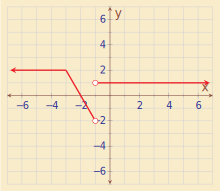
\includegraphics[scale=0.8]{../mathbook-caos-calculo/images/ejp-1-8-1g.pdf}}\hfill%
\subfigure[]{\includegraphics[scale=0.8]{../mathbook-caos-calculo/images/ejp-1-8-1h.pdf}}\hfill%
\subfigure[]{\includegraphics[scale=0.4]{../mathbook-caos-calculo/images/ejp-1-8-1c.pdf}}\\%
\subfigure[]{\includegraphics[scale=0.8]{../mathbook-caos-calculo/images/ejp-1-8-1e.pdf}}\hfill%
\subfigure[]{\includegraphics[scale=0.8]{../mathbook-caos-calculo/images/ejp-1-8-1f.pdf}}\hfill%
\subfigure[]{\includegraphics[scale=0.8]{../mathbook-caos-calculo/images/ejp-1-8-1j.pdf}}%
\end{figure}	
	

\item Un punto $P\left(  x,y\right)  $ se mueve, en sentido horario, sobre la
par\'{a}bola
\[
\left(  x-2\right)  ^{2}+16\left(  y+5\right)  =0.
\]
Exprese mediante una funci\'{o}n de variable real la distancia del punto
$P\left(  x,y\right)  $ al punto $A\left(  2,2\right)  .$

\item \label{cap1prob3}Una v\'{\i}a de ferrocarril cruza una carretera
formandose un \'{a}ngulo de $60^{0}$, como lo muestra la figura
\begin{center}
\includegraphics[scale=0.8]%
{../mathbook-caos-calculo/images/ejp-1-3.pdf}%
\end{center}

Una locomotora a $800$ metros de la intersecci\'{o}n se aleja de ella a
raz\'{o}n de $100\dfrac{km}{h}.$ Un automovil a $800$ metros de la
intersecci\'{o}n se acerca a ella a raz\'{o}n de $80\dfrac{km}{h}.$
\textquestiondown Cu\'{a}l es la distancia de separaci\'{o}n entre el
automovil y la locomotora en ese instante ?. Exprese mediante una funci\'{o}n
de variable real, dependiente del tiempo $t$, la distancia de separaci\'{o}n
entre la locomotora y el automovil$.$

\item Cierta cantidad de aceite fluye hacia el interior de un deposito en
forma de cono invertido a raz\'{o}n de $0.1\pi\,\frac{m^{3}}{\min}.$ El
deposito tiene un radio de $2.5m$ en su parte superior y una profundidad de
$10m$. Si el deposito inicialmente contiene $1.2m^{3}$ de aceite. Exprese
mediante una funci\'{o}n de variable real, dependiente de la altura $h$, la
cantidad de aceite del recipiente.%
\begin{center}
\includegraphics[scale=0.6]%
{../mathbook-caos-calculo/images/ejr-1-8-4.pdf}%
\end{center}




\item Sea $\triangle ABC$ is\'{o}sceles con $AB=AC,$ y $m\measuredangle
BAC=\alpha.$ Exprese mediante una funci\'{o}n de variable real, dependiente
del valor del \'{a}ngulo $\alpha,$ el \'{a}rea del $\triangle ABC$.

\item Una isla est\'{a} ubicada en el punto $A$, $4\,km$ mar adentro del punto
m\'{a}s cercano $B$ de una playa recta. Una atleta, en la isla desea ir al
punto $C$, a $6$ $km$ de $B$ playa abajo. La mujer debe dirigirse hacia un
punto $P$, entre $B$ y $C$, en un bote de remos a $3.5\dfrac{km}{h}$ y
desp\'{u}es caminar en forma recta de $P$ a $C$ a $6\dfrac{km}{h}.$ Exprese
mediante una funci\'{o}n de variable real, dependiente de $x=BP,$ el tiempo
necesario para viajar desde $A$ hacia $C,$ pasando por el punto $P$.
\begin{center}
\includegraphics[scale=0.3]%
{../mathbook-caos-calculo/images/ejp-1-6.pdf}%
\end{center}


\item Exprese mediante una funci\'{o}n de variable real, dependiente de $x,$
el \'{a}rea del rect\'{a}ngulo que tiene dos v\'{e}rtices en el eje $x$ y los
otros dos en la par\'{a}bola $y=16-x^{2},$ por arriba del eje $x.$

\item Hay que construir una pileta de las dimensiones que se muestran.
S\'{o}lo se puede variar el \'{a}ngulo $\theta$ . Exprese mediante una
funci\'{o}n de variable real, dependiente del \'{a}ngulo $\theta,$ el volumen
de la pileta.%
\begin{center}
\includegraphics[scale=0.3]%
{../mathbook-caos-calculo/images/ejr-1-8-8.pdf}%
\end{center}


\item Un granjero desea cercar tres terrenos rectangulares adyacentes
identicos, cada uno de ellos de 1800 pies cuadrados de \'{a}rea, incluyendo
cerca en medio de ellos. Exprese mediante una funci\'{o}n de variable real,
dependiente de la profundidad de los terrenos, el perimetro total para
realizar est\'{a} tarea.

\item Dada una esfera de radio $R$. Exprese mediante una funci\'{o}n de
variable real, dependiente de $R$, el volumen del cono circular recto de radio
$r$ y altura $h$ que puede inscribirse en la esfera.

\item Una particula se mueve a lo largo de una l\'{\i}nea recta, siendo su
posici\'{o}n $x\left(  t\right)  $ metros en todo tiempo $t>0$ segundos
\[
x\left(  t\right)  =\dfrac{5t+20}{t+1}+2t
\]


\begin{enumerate}
\item Completa la siguiente tabla:%
\[%
\begin{tabular}
[c]{|l|l|l|l|l|l|l|l|}\hline
$t\left[  s\right]  $ & $1$ & $2$ & $3$ & $4$ & $5$ & $6$ & $7$\\\hline
$x\left[  m\right]  $ &  &  &  &  &  &  & \\\hline
\end{tabular}
\ \
\]


\item Usa los resultados de la tabla para hacer un bosquejo de la gr\'{a}fica
de $x\left(  t\right)  .$ Con la ayuda de un software, gr\'{a}fique $x$ $vs$
$t.$ Compare y analice las gr\'{a}ficas.

\item \textquestiondown En qu\'{e} momento la part\'{\i}cula alcanza una
posici\'{o}n de $3$ metros?
\end{enumerate}

\item Una hoja de papel de dimensiones 12 cms por 8 cms , se corta por las
esquinas en cuadrados de $x$ cms de lado.

\begin{enumerate}
\item Muestre que el volumen que se puede construir a partir de la hoja viene
dado por $V(x)=4x(6-x)(4-x),0<x<4.$

\item Complete la siguiente tabla:%
\[%
\begin{tabular}
[c]{|l|l|l|l|l|l|}\hline
$x$ $\left[  cm\right]  $ & $0$ & $1$ & $2$ & $3$ & $4$\\\hline
$V$ $\left[  cm^{3}\right]  $ &  &  &  &  & \\\hline
\end{tabular}
\ .
\]


\item Estime el m\'{a}ximo volumen que puede tener la caja ( Explique sus procedimientos)
\end{enumerate}

\item Una funci\'{o}n est\'{a} definida por $f(x)=3x+1,$ $x\in R$. Determine
el conjunto soluci\'{o}n de la ecuaci\'{o}n $f(2x)-f(x+1)=4.$

\item Considere los conjuntos
\[
A=\{x\in\nz\mid x<5\},B=\{x\in\nz\mid3\leq x\leq5\}.
\]
Para cada una de las relaciones de $A$ a $B$ dadas a continuaci\'{o}n
determine su dominio y su rango. Haga una gr\'{a}fica de la relaci\'{o}n e
indique si la relaci\'{o}n dada es una funci\'{o}n. En caso de serlo indique
si es sobre, uno-a-uno o biyectiva. Justifique todas sus respuestas.

\begin{enumerate}
\item $R=\{(2,3),(3,5),(1,3),(4,4)\}$.

\item $S=\{(1,3),(2,3),(3,4),(4,5)\}$.

\item $T=\{(1,3),(1,4),(1,5)\}$.

\item $U=\{(1,3),(2,3),(3,3),(4,3)\}$.

\item $V=\{(1,4),(2,3)\}$.
\end{enumerate}

\item Considere, en cada caso, la funci\'{o}n de variable real $f$ definida
por la f\'{o}rmula dada. Determine dominio y rango de la funci\'{o}n e indique
si es sobre, uno-a-uno o biyectiva. Haga una gr\'{a}fica de la funci\'{o}n.
Indique tambi\'{e}n, si los hay, los valores m\'{a}ximo y m\'{\i}nimo de la funci\'{o}n.

\begin{enumerate}
\item $f(x)=x^{2}+3x+2$.

\item $f(x)=3x+7$.

\item $f(x)=3x^{2}+x-4$.

\item $f(x)=-x^{2}+x+1$.

\item $f(x)=\pi$.

\item $f(x)=2x^{2}-3x+5$.

\item $f(x)=|x-2|$.

\item $f(x)=|x^{2}+3x+2|$.
\end{enumerate}

\item Para cada una de las funciones del ejercicio anterior determine las
intersecciones de su gr\'{a}fica con los ejes coordenados. En cada caso
determine el dominio de la funci\'{o}n de variable real definida por la
f\'{o}rmula dada.

\begin{enumerate}
\item $f(x)=\sqrt{x^{2}+5x+6}$.

\item $f(x)=\dfrac{2-x}{x^{2}+5x+6}$.

\item $f(x)=\dfrac{\sqrt{2-x}}{x+3}$.

\item $f(x)=\dfrac{x+1}{3x^{2}+x+1}$.

\item $f(x)=\sqrt{|x|}$.

\item $f(x)=\sqrt{\dfrac{x-1}{2x+3}}$.

\item $f\left(  x\right)  =\sqrt{x^{2}+2x-15}$
\end{enumerate}

\item Considere la funci\'{o}n definida por $g(x)=x^{3}+x^{2}+1$.
\textquestiondown Est\'{a} $3$ en el rango de $g$? \textquestiondown Es $g$
una funci\'{o}n uno-a-uno?

\item Sea $f$ definida por $f(x)=\sqrt{2x+1}$. Encuentre los valores de $h$
para los cuales $2+h$ est\'{a} en:

\begin{enumerate}
\item El dominio de $f$.

\item El rango de $f$.
\end{enumerate}

\item En cada caso indique si la relaci\'{o}n real dada es una funci\'{o}n. En
caso afirmativo indique el dominio de la misma. En caso negativo, encuentre
una funci\'{o}n definida impl\'{\i}citamente por la ecuaci\'{o}n que define la relaci\'{o}n.

\begin{enumerate}
\item $R=\{(x,y)\mid x^{2}-y^{2}=1\}$.

\item $S=\{(x,y)\mid x^{2}+xy-3x=0\}$.

\item $T=\{(x,y)\mid x=1,x^{2}+x-y=0\}$.

\item $U=\{(t,u)\mid t^{2}+u^{2}-2u=0\}$.

\item $V=\{(t,s)\mid s^{3}+2s^{2}+s-t=0\}$.
\end{enumerate}

\item Considere la relaci\'{o}n $R=\{(x,y)\mid Ax^{2}+Cy^{2}+Dx+Ey+F=0\}$,
donde $A,C,D,E$ y $F$ son reales dados. Demuestre que:

\begin{enumerate}
\item Si $A=C\neq0$, la gr\'{a}fica de $R$ es una circunferencia, un punto o
el conjunto vac\'{\i}o.

\item Si $A=0$ o $C=0$, la gr\'{a}fica de $R$ es una par\'{a}bola, dos rectas
paralelas, una sola recta o el conjunto vac\'{\i}o.
\end{enumerate}

\item \label{ejercicio1} En cada caso determine el dominio de $f+g,fg$ y
$f/g$, para las funciones reales $f$ y $g$ definidas como se indica. Encuentre
adem\'{a}s
\[
(f+g)(x),(fg)(x),(f/g)(x)
\]
para $x$ en el dominio de la correspondiente funci\'{o}n.

\begin{enumerate}
\item $f(x)=\dfrac{x}{x-2},\ g(x)=\sqrt{x^{2}-x}$.

\item $f(x)=\dfrac{x-2}{x^{2}-3x+2},\ g(x)=\dfrac{2}{x+1}$.

\item $f(x)=\sqrt{x^{2}+3x+2},\ g(x)=\dfrac{x}{x+2}$.

\item $f(x)=\sqrt{x+1},\ g(x)=\sqrt{x^{2}+x+1}$.

\item $f(x)=\sqrt{\dfrac{x+1}{x-2}},\ g(x)=\sqrt{6+x-x^{2}}$.
\end{enumerate}

\item Como en el ejercicio anterior para las funciones
\[
f=\{(a,0),(b,1),(c,-3),(d,-5)\},\ g=\{(a,3),(b,-5),(c,6),(e,9)\}
\]


\item Sea $f$ la funci\'{o}n de variable real definida por $f(x)=5x+3$.
Determine todos los valores de $x$ para los cuales:

\begin{enumerate}
\item $f(2x)=2f(x)$.

\item $f(x+c)=f(x)+f(c)$, si $c$ es un real fijo dado.\newline Haga lo mismo
si $f(x)=5x$.
\end{enumerate}

\item Sea $f:\rz\longrightarrow\rz$ una funci\'{o}n. $f$ es una
\index{Aplicaci\'{o}n lineal|textbf}%
aplicaci\'{o}n lineal si, y solo si para todo $x_{1},x_{2}\in\rz$ se cumple
que $f(x_{1}+x_{2})=f(x_{1})+f(x_{2})$ y $f(x_{1}x_{2})=x_{1}f(x_{2})$.
Demuestre que el conjunto de todas las aplicaciones lineales de $\rz$ en
$\rz$, al cual notaremos $Lin(\rz,\rz)$, es cerrado para las operaciones de
adici\'{o}n de funciones y multiplicaci\'{o}n por funciones constantes. Es
decir, demuestre que si $f,g\in Lin(\rz,\rz)$ y $k\in\rz$ entonces:
\begin{align*}
(f+g)  &  \in Lin(\rz,\rz)\\
kf  &  \in Lin(\rz,\rz).
\end{align*}


\item Demuestre que una funci\'{o}n $f:\rz\longrightarrow\rz$ es una
aplicaci\'{o}n lineal si, y solo si existe una constante $k\in\rz$ tal que
$f(x)=kx$, para todo $x\in\rz$. As\'{\i}, toda aplicaci\'{o}n lineal es una
funci\'{o}n lineal. \textquestiondown Es verdadero el rec\'{\i}proco?.

\item En cada caso determine, si est\'{a}n definidas, las compuestas $f\circ
g$ y $g\circ f$, indicando sus dominios de definici\'{o}n.

\begin{enumerate}
\item $f=\{(a,1),(2,-3),(c,d),(0,5)\},\ g=\{(1,3),(5,6),(a,4)\}$.

\item $f=\{(3,2),(4,5),(6,7)\},\ g=\{(2,4),(5,6),(8,3)\}$.

\item $f$ y $g$ son funciones de variable real definidas por:

\begin{enumerate}
\item $f(x)=2,\ g(x)=5x$.

\item $f(x)=3,\ g(x)=2$.

\item $f(x)=x+1,\ g(x)=x-1$.

\item $f(x)=x^{2}+2x-3,\ g(x)=\sqrt{x}$.

\item $f(x)=\sqrt{x-2},\ g(x)=x^{3}$.

\item $f(x)=\dfrac{x}{x+3},g(x)=\sqrt{x+1}$.
\end{enumerate}
\end{enumerate}

\item En cada caso indique si la funci\'{o}n dada es invertible. En caso
afirmativo, encuentre su inversa. Si no es invertible, encuentre al menos dos
restricciones de la funci\'{o}n dada que sean invertibles y halle las inversas
de tales restricciones. Utilice software adecuado para graficar la funci\'{o}n
(o una restricci\'{o}n de la misma) y su inversa.

\begin{enumerate}
\item $f=\{(1,3),(\pi,5),(\sqrt{2},3),(5,7)\}$.

\item $g=\{(2,1),(3,5),(4,0),(6,1),(8,5)\}$.

\item La funci\'{o}n de variable real $f$ definida por:

\begin{enumerate}
\item $f(x)=5x-7$.

\item $f(x)=6$.

\item $f(x)=x$.

\item $f(x)=ax+b$, donde $a,b\in\rz$.

\item $f(x)=x^{2}-x-30$.

\item $f(x)=ax^{2}+bx+c$, donde $a,b$ y $c$ son reales cualesquiera con
$a\neq0$.

\item $f(x)=\sqrt{x}$.

\item $f(x)=x^{3}$.
\end{enumerate}
\end{enumerate}

\item Una funci\'{o}n $f:\rz\longrightarrow\rz$ se denomina localmente
invertible si existe un intervalo abierto $\left]  a,b\right[  $ tal que la
restricci\'{o}n $f|_{\left]  a,b\right[  }$ es invertible. En tal caso
$f|_{\left]  a,b\right[  }^{-1}$ es una inversa local de $f$. Encuentre al
menos dos inversas locales para la funci\'{o}n $f$ definida por:

\begin{enumerate}
\item $f(x)=x^{2}+3x+5$.

\item $f(x)=x^{3}$.
\end{enumerate}

\item Sea $f$ una funci\'{o}n real invertible \textquestiondown Se puede
afirmar que $f^{-1}=\dfrac{1}{f}$? Justifique su respuesta.

\item Sea $a$ un real positivo. Una funci\'{o}n $f:[-a,a]\longrightarrow\rz$
se denomina%
\index{Funci\'{o}n!-- par}
par si, y solo si
\[
f(-x)=f(x)\ \mbox{para todo \ }x\in\lbrack-a,a].
\]
$f$ es una funci\'{o}n impar%
\index{Funci\'{o}n!-- impar}
si, y solo si
\[
f(-x)=-f(x)\ \mbox{para todo \ }x\in\lbrack-a,a].
\]


\begin{enumerate}
\item Demuestre que si $f(x)=x^{2}+1$, entonces $f$ es par y que la
funci\'{o}n $g$ definida por $g(x)=x^{3}+x$ es impar.

\item \textquestiondown Es toda funci\'{o}n constante una funci\'{o}n par?

\item Demuestre que una funci\'{o}n lineal es par si, y solo si es constante e
impar si, y solo si es un m\'{u}ltiplo de la funci\'{o}n id\'{e}ntidad. En
particular, la funci\'{o}n identidad es impar.

\item Demuestre que la funci\'{o}n cuadr\'{a}tica $f(x)=ax^{2}+bx+c$ es una
funci\'{o}n par si, y solo si $b=0$. \textquestiondown Existen funciones
cuadr\'{a}ticas impares?.

\item Discuta la veracidad de la siguiente afirmaci\'{o}n:

Si $f$ es una funci\'{o}n par, su gr\'{a}fica es sim\'{e}trica respecto del
eje $Y$.
\end{enumerate}

\item En cada caso indique si la proposici\'{o}n dada es Verdadera o falsa.
Justifique sus respuestas.

\begin{enumerate}
\item Toda funci\'{o}n lineal es invertible.

\item Una funci\'{o}n lineal es invertible si, y solo si no es constante.

\item Toda funci\'{o}n lineal no constante es localmente invertible.

\item Toda funci\'{o}n cuadr\'{a}tica es invertible.

\item Ninguna funci\'{o}n cuadr\'{a}tica es invertible.

\item Toda funci\'{o}n cuadr\'{a}tica es localmente invertible.

\item Una funci\'{o}n real de variable real es invertible si, y solo si toda
recta paralela al eje $X$ que intersecte su gr\'{a}fica lo hace en un solo punto.

\item Una funci\'{o}n $f:\rz\longrightarrow\rz$ es par si, y solo toda recta
paralela al eje $X$ que intersecte la gr\'{a}fica de $f$ lo hace en al menos
dos puntos.
\end{enumerate}

\item Sea la funci\'{o}n $f(x)=2x^{2}+x-3$ y $g\left(  x\right)  =x^{3}-1$

\begin{enumerate}
\item Calcule $f+g,fg,\frac{f}{g}$ y sus respectivos dominios.

\item Calcule $\dfrac{f\left(  3+h\right)  -f\left(  3\right)  }{h}.$

\item Halle $\left(  f\circ f\right)  \left(  x\right)  ,\left(  f\circ
g\right)  \left(  x\right)  ,\left(  g\circ f\right)  \left(  x\right)
,\left(  g\circ g\right)  \left(  x\right)  $ y sus respectivos dominios.

\item Calcule $f\left(  f\left(  1\right)  \right)  ,\left(  f\circ g\right)
\left(  0\right)  ,\left(  g\circ f\right)  \left(  -1\right)  ,\left(  g\circ
g\right)  \left(  1\right)  .$
\end{enumerate}

\item Sean $f\left(  x\right)  =x^{4}+2x^{3}-3x^{2}-4x-5.$ y $g\left(
x\right)  =3x^{4}+2x^{3}+7x-5.$

\begin{enumerate}
\item Hallar $h_{1}\left(  x\right)  :=\dfrac{1}{2}\left[  f\left(  x\right)
+g\left(  x\right)  \right]  .$

\item Hallar $h_{2}\left(  x\right)  :=\dfrac{1}{2}\left[  f\left(  x\right)
-g\left(  x\right)  \right]  .$
\end{enumerate}

\item Consideremos la funci\'{o}n $f$ definida por $f(x)$ $=\dfrac{x^{2}%
-x+1}{x+2}$ para $x\geq0.$ \textquestiondown Existe alg\'{u}n valor$\ a$ del
dominio de la funci\'{o}n tal que $f(a)=a$?$.$

\item \label{cap1prob35}Sean las funciones: $f(x)=\dfrac{x^{2}-1}{x+1}$ y
$g(x)=$ $-\sqrt{x^{2}-\frac{1}{4}}.$ Hallar:\vspace{-0.9in}

\multicolsep2.5 cm \columnsep1 cm\begin{multicols}
{2}
\begin{enumerate}
\item$\operatorname*{Dom}(f)$
\item$\operatorname*{Dom}(g)$
\item$\left(  f + g\right)            \left(
x\right)            $ \item $\operatorname*{Dom}(f + g)$
\item$\left(            gf\right) \left(   x\right)
$ \item$\operatorname*{Dom}(gf)$ \item$g\left(  g\left(
x\right)            \right) $
\item$\left(  f\circ g\right)            \left(
x\right)
$ \item $\operatorname*{Dom}(f\circ g)$
\item$\left(            g\circ f\right) \left(   x\right)$
\item$\operatorname*{Dom}(g\circ f)$
\item $\operatorname*{Dom}(f/g)$
\end{enumerate}
\end{multicols}\vspace{-0.9in}

\item Realice el problema \ref{cap1prob35}, si:

\begin{enumerate}
\item $f\left(  x\right)  =\dfrac{1+2x}{x^{2}}$ y $g\left(  x\right)
=\sqrt{x-1}.$

\item $f\left(  x\right)  =\dfrac{x^{2}+9}{x^{4}-1}$ y $g\left(  x\right)
=\sqrt{8-x^{2}}.$

\item $f\left(  x\right)  =\dfrac{1}{x^{4}-13x^{2}+36}$ y $g\left(  x\right)
=\sqrt{x^{2}-1}.$
\end{enumerate}

\item Para cada una de las funciones $f,g,h$ dadas a continuaci\'{o}n halle el
dominio, el rango, y con ayuda de un software, elabore la gr\'{a}fica.

\begin{enumerate}
\item
\[
f\left(  x\right)  =\left\{
\begin{tabular}
[c]{cl}%
$\dfrac{x^{2}-9}{x-3}$ & , si $x\neq3$\\
\multicolumn{1}{l}{$1$} & , si $x=3.$%
\end{tabular}
\right.
\]


\item
\[
g\left(  x\right)  =\left\{
\begin{tabular}
[c]{ll}%
$\sqrt{x^{2}-4}$ & , si $x<1$\\
$2x-1$ & , si $x\geq1.$%
\end{tabular}
\ \ \right.
\]


\item
\[
h\left(  x\right)  =\dfrac{\left\vert x\right\vert }{x}%
\]

\end{enumerate}

\item Considerando las funciones del ejemplo anterior calcule $f+g,fg,h\circ
g,g\circ f$ y determine, para cada caso, el dominio respectivo.

\item Sea la funci\'{o}n%
\[
g\left(  x\right)  =\left\{
\begin{tabular}
[c]{ll}%
$x^{2}+3x-2$ & , si $0<x<1$\\
$x-1$ & , si $x\geq1.$%
\end{tabular}
\ \ \ \ \ \ \right.
\]
Calcule el dominio de $g$. \textquestiondown \ Las expresiones $g\left(
1\right)  ,g\left(  -1\right)  ,g\left(  0\right)  ,g\left(  \dfrac{1}%
{2}\right)  $ est\'{a}n bien definidas?. En caso afirmativo determine la
imagen, en caso negativo, Justifique.

\item Sea la funci\'{o}n $f\left(  x\right)  =\left\vert 3x-2\right\vert
+\left\vert x+1\right\vert $

\begin{enumerate}
\item Reescriba la funci\'{o}n sin barras de valor absoluto .

\item Elabore la gr\'{a}fica.

\item Calcule $f(\frac{2}{3}),f(\frac{3}{2}),f\left(  2\right)  ,f\left(
3\right)  .$
\end{enumerate}

\item Determine los dominios de cada una de las funciones dadas

\begin{enumerate}
\item
\[
h\left(  x\right)  =\sqrt{\allowbreak6x^{3}-5x^{2}-2x+1}.
\]


\item
\[
g\left(  u\right)  =\dfrac{5u+1}{\allowbreak6u^{3}+11u^{2}-3u-2}.
\]


\item
\[
f\left(  u\right)  =\dfrac{\sqrt{\allowbreak6u^{3}-5u^{2}-2u+1}}%
{\allowbreak6u^{3}+11u^{2}-3u-2}.
\]


\item
\[
s\left(  y\right)  =\dfrac{\sqrt{3y^{3}+y^{2}-6y-2}}{2y^{2}+y-3}.
\]


\item
\[
g\left(  t\right)  =\sqrt{\dfrac{5t-2}{t^{2}-1}}.
\]


\item
\[
g\left(  x\right)  =\sqrt{\dfrac{5x^{2}+2}{x^{2}-4}}.
\]


\item
\[
f\left(  x\right)  =\sqrt{\dfrac{x-2}{\left(  x^{2}+x-1\right)  \left(
1-2x^{2}\right)  }}.
\]


\item
\[
h\left(  z\right)  =\sqrt[3]{\dfrac{5z-2}{z^{2}-1}}.
\]


\item
\[
s\left(  x\right)  =\sqrt[7]{\dfrac{x^{5}+2x^{2}+2}{x^{2}+7x-1}}.
\]


\item
\[
t\left(  y\right)  =\dfrac{\sqrt{2y^{2}+y-1}}{\sqrt{7y-10y^{2}-1}}.
\]

\end{enumerate}

\item Si $F(x)=\sqrt{(x-3)(x-1)}$

\begin{enumerate}
\item Determine el dominio de $F$.

\item Pruebe que $F(2-\sqrt{10})=3$
\end{enumerate}

\item Si $g\left(  x\right)  =x^{2}+x-1$, calcule:

\begin{enumerate}
\item $\dfrac{g\left(  x+h\right)  -g\left(  x\right)  }{h}.$

\item $\dfrac{g\left(  x+\dfrac{1}{h}\right)  -g\left(  \dfrac{1}{h}\right)
}{x}.$

\item $g\left(  2x\right)  -g\left(  3x\right)  .$
\end{enumerate}

\item Pruebe que si $c\in\rz,\left\{  a_{i}\right\}  _{i\in\nz}$ y $\left\{
b_{i}\right\}  _{i\in\nz}$ sucesiones de n\'{u}meros reales, entonces

\begin{enumerate}
\item
\[
\sum_{i=1}^{n}{c=cn.}%
\]


\item
\[
\sum_{i=1}^{n}{ca_{i}=c}\sum_{i=1}^{n}{a_{i}.}%
\]


\item
\[
\sum_{i=1}^{n}\left(  {a_{i}+b_{i}}\right)  {=}\sum_{i=1}^{n}{a_{i}+}%
\sum_{i=1}^{n}{b_{i}.}%
\]

\end{enumerate}

\item Pruebe, utilizando inducci\'{o}n matem\'{a}tica, que el t\'{e}rmino
n-\'{e}simo de la serie asociada a la sucesi\'{o}n:

\begin{enumerate}
\item $\left\{  i\right\}  _{i\in\nz}$ est\'{a} dado por
\[
\frac{n(n+1)}{2}.
\]


\item $\left\{  i^{2}\right\}  _{i\in\nz}$ est\'{a} dado por
\[
\frac{n(n+1)(2n+1)}{6}.
\]


\item $\left\{  i^{3}\right\}  _{i\in\nz}$ est\'{a} dado por
\[
\frac{1}{4}n^{2}+\frac{1}{2}n^{3}+\frac{1}{4}n^{4}.
\]

\end{enumerate}

\item Calcule:

\begin{enumerate}
\item
\[
\sum_{k=4}^{22}{(k-8)^{2}.}%
\]


\item
\[
\sum_{n=1}^{5}\left(  n+3\right)  .
\]


\item
\[
\sum_{n=1}^{15}\left(  2n-1\right)  ^{2}.
\]


\item
\[
\sum_{n=1}^{350}n.
\]

\end{enumerate}

\item Encuentre una sucesi\'{o}n con dominio $\nz$ cuyo rango sea el mismo de
los conjuntos dados (los mismos t\'{e}rminos en el mismo orden). Adem\'{a}s
para cada una de las sucesiones, determine sus cinco primeros t\'{e}rminos.
Finalmente, determine los cinco primeros t\'{e}rminos de la serie asociada a
la sucesi\'{o}n.

\begin{enumerate}
\item $\{n^{2}\}_{n=0}^{\infty}$.

\item $\left\{  \frac{2n}{n-1}\right\}  _{n=2}^{\infty}$.

\item $\left\{  \frac{n}{n+1}\right\}  _{n=0}^{\infty}$.

\item $\left\{  \sqrt{n}\right\}  _{n=0}^{\infty}$.

\item $\left\{  \frac{n}{\sqrt{n-3}}\right\}  _{n=4}^{\infty}$.
\end{enumerate}

\item Un subconjunto $A$ de $\rz$ se denomina
\index{Conjunto!-- enumerable}%
contable o
\index{Conjunto!-- contable}%
enumerable si est\'{a} contenido en el rango de una sucesi\'{o}n. El conjunto
$A$ es finito, si es vac\'{\i}o o si existen un n\'{u}mero natural \ $k$ \ y
\ una funci\'{o}n biyectiva $f:\{x\in\nz\mid x\leq k\}\longrightarrow A$. Demuestre:

\begin{enumerate}
\item Todo conjunto finito de n\'{u}meros reales es contable.

\item $A$ es contable si, y solo si existen un subconjunto $J\subseteq\nz$ y
una funci\'{o}n biyectiva $\beta:J\longrightarrow A$.

\item los conjuntos $\nz,\gz$ y $\qz$ son contables.
\end{enumerate}

\item Cuales son los primeros $6$ terminos de cada una de las sucesiones que
poseen el t\'{e}rmino n-\'{e}simo dado.

\begin{enumerate}
\item $a_{n}=\dfrac{n-2}{n}.$

\item $a_{n}=\cos\left[  \left(  2n-1\right)  \dfrac{\pi}{2}\right]  .$

\item $a_{n}=\dfrac{\left(  -1\right)  ^{n-1}\sin\left(  \pi n\right)  }{n}$

\item $a_{n}=\sqrt[n]{n}.$

\item $a_{n}=\dfrac{3^{n}}{n!}.$

\item $a_{n}=\dfrac{\cos\left(  n\right)  }{n}.$

\item $a_{n}=%
%TCIMACRO{\dsum \limits_{k=1}^{n}}%
%BeginExpansion
{\displaystyle\sum\limits_{k=1}^{n}}
%EndExpansion
\dfrac{1}{k^{2}}.$

\item $a_{n}=%
%TCIMACRO{\dsum \limits_{k=1}^{n}}%
%BeginExpansion
{\displaystyle\sum\limits_{k=1}^{n}}
%EndExpansion
\dfrac{1}{k\left(  k+1\right)  }.$

\item $a_{n}=%
%TCIMACRO{\dsum \limits_{k=0}^{n}}%
%BeginExpansion
{\displaystyle\sum\limits_{k=0}^{n}}
%EndExpansion
\left(  \dfrac{2}{3}\right)  ^{k}.$
\end{enumerate}

\item Calcule la primeras 6 sumas parciales de las siguientes series.

\begin{enumerate}
\item $%
%TCIMACRO{\dsum \limits_{n=1}^{\infty}}%
%BeginExpansion
{\displaystyle\sum\limits_{n=1}^{\infty}}
%EndExpansion
\dfrac{1}{n^{2}}.$

\item $%
%TCIMACRO{\dsum \limits_{n=1}^{\infty}}%
%BeginExpansion
{\displaystyle\sum\limits_{n=1}^{\infty}}
%EndExpansion
\dfrac{1}{\left(  4n-3\right)  \left(  4n+1\right)  }.$

\item $%
%TCIMACRO{\dsum \limits_{n=1}^{\infty}}%
%BeginExpansion
{\displaystyle\sum\limits_{n=1}^{\infty}}
%EndExpansion
\dfrac{n}{n+1}.$

\item $%
%TCIMACRO{\dsum \limits_{n=1}^{\infty}}%
%BeginExpansion
{\displaystyle\sum\limits_{n=1}^{\infty}}
%EndExpansion
\left(  \dfrac{2}{5}\right)  ^{n}$

\item $%
%TCIMACRO{\dsum \limits_{n=1}^{\infty}}%
%BeginExpansion
{\displaystyle\sum\limits_{n=1}^{\infty}}
%EndExpansion
\dfrac{1}{3^{n}}.$

\item $%
%TCIMACRO{\dsum \limits_{n=1}^{\infty}}%
%BeginExpansion
{\displaystyle\sum\limits_{n=1}^{\infty}}
%EndExpansion
\left(  \dfrac{1}{n}-\dfrac{1}{n+1}\right)  .$

\item $%
%TCIMACRO{\dsum \limits_{n=0}^{\infty}}%
%BeginExpansion
{\displaystyle\sum\limits_{n=0}^{\infty}}
%EndExpansion
\dfrac{4^{n+1}}{5^{n}}.$

\item $%
%TCIMACRO{\dsum \limits_{n=1}^{\infty}}%
%BeginExpansion
{\displaystyle\sum\limits_{n=1}^{\infty}}
%EndExpansion
\dfrac{1}{e^{2n}}.$
\end{enumerate}
\end{enumerate}


%
\chapter{L\'{\i}mite y Continuidad}

En este cap\'{\i}tulo se presenta uno de los conceptos fundamentales del
C\'{a}lculo y, en general, del An\'{a}lisis matem\'{a}tico: El concepto de
l\'{\i}mite. En principio-y ese ser\'{a} el tratamiento del concepto en este
curso- la idea de l\'{\i}mite est\'{a} ligada a la de \textquotedblleft
distancia\textquotedblright\ o, m\'{a}s precisamente, a la de
\textquotedblleft cercan\'{\i}a \textquotedblright, por lo que nuestro
inter\'{e}s inicial estar\'{a} en definir formalmente lo que consideraremos
una \textquotedblleft distancia\textquotedblright\ tanto en el sentido
intuitivo, ligado a problemas de naturaleza f\'{\i}sica o geom\'{e}trica, como
en la abstracci\'{o}n del mismo.

\section{Topolog\'{\i}a de la recta real}

Para dos puntos cualesquiera $P$ y $Q$ de la recta real, la
\index{Distancia|textbf}%
distancia entre ellos viene dada por el real no negativo
\begin{equation}
d(P,Q)=|x_{1}-x_{2}|, \label{distanciaenR}%
\end{equation}
donde $x_{1}$ y $x_{2}$ son las coordenadas de los puntos $P$ y $Q$,
respectivamente. Diremos tambi\'{e}n que tal distancia es la distancia entre
los reales $x_{1}$ y $x_{2}$. La distancia definida en $\rz$ por la
ecuaci\'{o}n (\ref{distanciaenR}) tiene algunas propiedades b\'{a}sicas
importantes, las cuales se desprenden de las propiedades del valor absoluto de
reales. Algunas de \'{e}stas \'{u}ltimas se enuncian a continuaci\'{o}n.
Suponemos $x,y\in\rz$:
\begin{align}
|x|  &  \geq0\\
|x|=0  &  \Longleftrightarrow x=0\\
|x+y|  &  \leq|x|+|y|\label{triangular1}\\
|xy|  &  =|x||y|
\end{align}
De las anteriores se siguen las siguientes propiedades de la distancia en
$\rz$.%
\index{Distancia!Propiedades de la --}%


\begin{theorem}
Sean $x,y,z$ n\'{u}meros reales, entonces:
\begin{align}
|x-y|  &  \geq0\label{nonegativa}\\
|x-y|=0  &  \Longleftrightarrow x=y\label{nulidad}\\
|x-y|  &  =|y-x|\label{simetria}\\
|x-y|  &  \leq|x-z|+|y-z| \label{triangular}%
\end{align}

\end{theorem}

La desigualdad (\ref{triangular1}) (y tambi\'{e}n su consecuencia
(\ref{triangular})) se acostumbra a denominar desigualdad triangular.

Definimos a continuaci\'{o}n conceptos importantes en la forma\-lizaci\'{o}n
del concepto de l\'{\i}mite, entre ellos el de vecindad.

\begin{definition}
Sean $c,r\in\rz$, con $r>0$. El intervalo abierto \textbf{centrado} en $c$ y
con radio $r$ es el intervalo
\[
]c-r,c+r[.
\]
Todo subconjunto de $\rz$ que contenga un intervalo abierto centrado en $c$ se
denomina una
\index{Vecindad|textbf}%
\textbf{vecindad} de $c$. En particular, todo intervalo abierto centrado en
$c$ es una vecindad de $c$.
\end{definition}
%TODO ---------
Se sigue f\'{a}cilmente que el intervalo con centro en $c$ y radio $r$ es el
conjunto de reales cuya distancia al centro es menor que el radio. En efecto,
tenemos:
\begin{align*}
x\in]c-r,c+r[  &  \Longleftrightarrow c-r<x<c+r\\
&  \Longleftrightarrow-r<x-c<r\\
&  \Longleftrightarrow|x-c|<r
\end{align*}
El intervalo $]a,b[=\{x\in\rz\mid a<x<b\}$ es claramente un intervalo abierto
centrado en $c=\frac{a+b}{2}$ y con radio $r=\frac{b-a}{2}$:
\begin{align*}
c-r  &  =\frac{a+b}{2}-\frac{b-a}{2}\\
&  =a\\
c+r  &  =\frac{a+b}{2}+\frac{b-a}{2}\\
&  =b
\end{align*}
%

\begin{figure}[H]
\centering
\includegraphics[scale=0.8]%
{fig2-1.pdf}%
\caption{Vecindades de $c$}%
\label{tiende2}%
\end{figure}



Podemos ahora formalizar, en t\'{e}rmino de vecindades, la noci\'{o}n de
proxi\-midad entre puntos de la recta real o, si se prefiere, entre
n\'{u}meros reales. Si $c$ es un real fijo, un real $x$ es \textquotedblleft%
\textit{cercano}\textquotedblright\ a $c$ si est\'{a} contenido en una
vecindad \textquotedblleft\textit{peque\~{n}a}\textquotedblright\ de $c$,
m\'{a}s precisamente, si pertenece a un intervalo centrado en $c$ y de radio
peque\~{n}o. As\'{\i}, la expresi\'{o}n \textquotedblleft\emph{la variable
real }$x$\emph{ tiende a }$c$\textquotedblright\ se interpreta diciendo que
$x$ toma valores en intervalos centrados en $c$ con radios cada vez menores
(ver figura \ref{tiende2}).

Terminamos esta secci\'{o}n con el concepto de punto de acumulaci\'{o}n de un
conjunto de n\'{u}meros reales. Intuitivamente hablando, un real $c$ es punto
de acumulaci\'{o}n de un conjunto $A$, si en las vecindades de $c$ se acumulan
en \textquotedblleft gran cantidad\textquotedblright\ elementos de tal conjunto.

\begin{definition}
Sean $A\subseteq\rz$ y $c\in\rz$. $c$ es un%
\index{Punto de acumulaci\'{o}n|textbf}
\underline{punto de} \underline{acumulaci\'{o}n} de $A$ si, y s\'{o}lo si toda
vecindad de $c$ contiene elementos de $A$ distintos de $c$.
\end{definition}

De la definici\'{o}n anterior, se sigue que si $c$ es punto de acumulaci\'{o}n
de $A$ toda vecindad de $c$ contiene infinitos elementos de $A$. En
consecuencia, ning\'{u}n conjunto finito tiene puntos de acumulaci\'{o}n.

\section{L\'{\i}mite de sucesiones}

Consideremos, como ejemplo introductorio, la sucesi\'{o}n $\left\{  \frac
{1}{n}\right\}  _{n\in\nz}$. Intuitivamente es claro que a medida que $n$ toma
valores m\'{a}s grandes, los valores de la sucesi\'{o}n son cada vez m\'{a}s
cercanos a cero. La tabla siguiente lo ilustra.

\begin{center}%
\begin{tabular}
[c]{|l||l|l|l|l|l|l|l|}\hline
$n$ & $1$ & $2$ & $3$ & $\dots$ & $50$ & $10^{6}$ & $10^{10}$\\\hline
$\frac{1}{n}$ & $1$ & $0.5$ & $0.333...$ & $\dots$ & $0.02$ & $0.000001$ &
$0.0000000001$\\\hline
\end{tabular}



\end{center}

El que, como lo sugiere la tabla anterior, $\frac{1}{n}$ tienda a cero
significa que toda vecindad de cero contiene a la \textquotedblleft
mayor\'{\i}a\textquotedblright\ de los t\'{e}rminos de la sucesi\'{o}n.
N\'{o}tese, en efecto, que si conside\-ramos intervalos centrados en cero y
con radios arbitrariamente peque\~{n}os, en cada caso solo un n\'{u}mero
finito de t\'{e}rminos de la sucesi\'{o}n se quedan por fuera del intervalo.
As\'{\i}, por ejemplo, para un radio $r=\frac{1}{5}$, todos los t\'{e}rminos
$\frac{1}{n}$ para $n\geq6$, est\'{a}n en el intervalo con centro en $0$ y
dicho radio $\frac{1}{5}$ (ver figura \ref{vecinocero2}).%


%TODO
\begin{figure}[H]
\centering
\includegraphics[scale=0.8]%
{fig-2-2.pdf}%
\caption{Vecindades de $c$}%
\label{vecinocero2}%
\end{figure}
%TODO 
En general, si $r>0$, existe un n\'{u}mero natural $N$ tal que $N>\frac{1}{r}%
$, por lo que para todo $n\geq N$ se tiene que
\begin{align*}
n>\frac{1}{r}  &  \Longrightarrow\frac{1}{n}<r\\
&  \Longrightarrow\left\vert \frac{1}{n}-0\right\vert <r
\end{align*}
lo que muestra que todos los t\'{e}rminos de la sucesi\'{o}n, a partir del
valor $n=N$, est\'{a}n en el intervalo centrado en $0$ y con radio $r$. Este
hecho se expresa diciendo que
\[
\lim_{n\rightarrow\infty}\frac{1}{n}=0
\]


La definici\'{o}n formal de l\'{\i}mite de una sucesi\'{o}n es como sigue. Sin
p\'{e}rdida de generalidad, como se explic\'{o} en el cap\'{\i}tulo anterior,
supondremos que el dominio de la sucesi\'{o}n es $\nz$.

\begin{definition}
\label{limitesucesion}%
\index{Sucesi\'{o}n!-- convergente}
Sea $\{x_{n}\}_{n\in\nz}$ una sucesi\'{o}n real. Decimos que la sucesi\'{o}n
es \textbf{convergente} si, y s\'{o}lo si existe un real $L$, tal que para
todo $r>0$, existe un n\'{u}mero natural $N$ tal que
\begin{equation}
|x_{n}-L|<r,\mbox{ \ siempre que \ }n\geq N \label{deflimitesucesion}%
\end{equation}
El real $L$ es el l\'{\i}mite de la sucesi\'{o}n%
\index{Sucesi\'{o}n!L\'{\i}mite de una --}
$\{x_{n}\}_{n\in\nz}$. Tal l\'{\i}mite es \'{u}nico (ver ejercicios) y decimos
que $x_{n}$ converge a $L$ y escribiremos
\[
\lim_{n\rightarrow\infty}x_{n}=L.
\]
Tambi\'{e}n es costumbre abreviar la expresi\'{o}n anterior escribiendo
$x_{n}\rightarrow L$.
\end{definition}

Como se anticip\'{o}, la ecuaci\'{o}n \ref{deflimitesucesion} establece que
todo intervalo abierto centrado en (toda vecindad de ) $L$ contiene a todos
los t\'{e}rminos de la sucesi\'{o}n, excepto a un n\'{u}mero finito de ellos.
Una sucesi\'{o}n no convergente se denomina divergente%
\index{Sucesi\'{o}n!-- divergente}%
.

La definici\'{o}n \ref{limitesucesion} no suministra herramientas
pr\'{a}cticas para el c\'{a}lculo de l\'{\i}mites. De hecho, la existencia
misma del l\'{\i}mite, como veremos, podr\'{\i}a establecerse sin conocerlo
espec\'{\i}ficamente. En la pr\'{a}ctica, necesitamos algunas herramientas que
nos permitan determinar tanto la existencia del l\'{\i}mite, como el
l\'{\i}mite mismo. Los teoremas que siguen apuntan en esa direcci\'{o}n,
aunque debe advertirse que, en general, no existen f\'{o}rmulas o
\textquotedblleft reglas m\'{a}gicas\textquotedblright\ que nos permitan
determinar l\'{\i}mites de sucesiones reales en cualquier caso.

Una de las propiedades b\'{a}sicas de una sucesi\'{o}n convergente es el que
su rango es un conjunto acotado%
\index{Conjunto!-- acotado}%
, lo cual significa que est\'{a} contenido en un intervalo de longitud finita.

\begin{theorem}
Sea $\{x_{n}\}_{n\in\nz}$ una sucesi\'{o}n convergente, entonces existe una
constante positiva $K$ tal que para todo $n\in\nz$ se tiene
\begin{equation}
|x_{n}|\leq K \label{acotada}%
\end{equation}

\end{theorem}

\begin{proof}
Sea $L$ el l\'{\i}mite de la sucesi\'{o}n $\{x_{n}\}_{n\in\nz}$. Entonces,
para $r=1$, se tiene que existe un n\'{u}mero natural $N$ tal que
\[
|x_{n}-L|<1,
\]
para $n\geq N$. Se tiene entonces que para $n\geq N$:
\begin{align*}
|x_{n}|  &  =|x_{n}-L+L|\\
&  \leq|x_{n}-L|+|L|\\
&  \leq1+L
\end{align*}
Escogiendo $K=Max\{1+L,|x_{n}|\mid n<N\}$ se tiene que $|x_{n}|\leq K$, para
todo natural $n$.
\end{proof}

El siguiente resultado puede ser de gran utilidad. B\'{a}sicamente, transforma
el problema de la convergencia de una sucesi\'{o}n a un real $L$ en el de la
convergencia a cero. Es una consecuencia inmediata de la definici\'{o}n.

\begin{theorem}
Sean $\{x_{n}\}_{n\in\nz}$ una sucesi\'{o}n y $L$ un n\'{u}mero real.
Entonces:
\begin{equation}
\lim_{n\rightarrow\infty}x_{n}=L\Longleftrightarrow\lim_{n\rightarrow\infty
}|x_{n}-L|=0
\end{equation}

\end{theorem}

El teorema anterior establece un hecho intuitivamente claro: Los valores de la
sucesi\'{o}n se aproximan a $L$ si, y solo si la distancia entre los
t\'{e}rminos de la sucesi\'{o}n y $L$ es pr\'{o}xima a cero. El teorema
siguiente ser\'{a} de gran utilidad en el c\'{a}lculo de l\'{\i}mites de
sucesiones cuando se conocen los l\'{\i}mites de otras sucesiones dadas.

\begin{theorem}%
\index{Sucesiones!Algebra de --}%
\label{algebrasucesiones} Sean $\{x_{n}\}_{n\in\nz},\{y_{n}\}_{n\in\nz}$
sucesiones reales convergentes a $L_{1}$ y $L_{2}$, respectivamente.
Entonces:
\begin{align}
x_{n}+y_{n}  &  \rightarrow L_{1}+L_{2}\label{sumasucesion}\\
x_{n}-y_{n}  &  \rightarrow L_{1}-L_{2}\\
x_{n}y_{n}  &  \rightarrow L_{1}L_{2}\label{productosucesion}\\
cx_{n}  &  \rightarrow cL_{1},c\in\rz
\end{align}

\end{theorem}

Tambi\'{e}n es claro que si una sucesi\'{o}n $\{x_{n}\}$ converge a cero su
producto por una sucesi\'{o}n convergente $\{y_{n}\}$ es tambi\'{e}n
convergente a cero. Sin embargo, una condici\'{o}n m\'{a}s d\'{e}bil que la
convergencia para $\{y_{n}\}$, como el ser acotada, garantiza tambi\'{e}n la
convergencia a cero del producto. Antes demostramos un importante criterio de comparaci\'{o}n.

\begin{theorem}
\label{emparedado}%
\index{Teorema!-- del emparedado}
Sean $\{x_{n}\}_{n\in\nz},\{y_{n}\}_{n\in\nz}$ sucesiones reales. Si existe un
$n_{0}\in\nz$ tal que
\[
|y_{n}|\leq|x_{n}|,\mbox{ \ para todo \ }n\geq n_{0},
\]
entonces $y_{n}\rightarrow0$ si $x_{n}\rightarrow0$.
\end{theorem}

\begin{proof}
Supongamos que $x_{n}$ converge a cero. Entonces para $r>0$ se tiene que
existe $N\in\nz$ tal que $|x_{n}|<r$, siempre que $n\geq N$. Si escogemos
$N_{1}=Max\{N,n_{0}\}$ entonces para $n\geq N_{1}$ tenemos
\[
|y_{n}|\leq|x_{n}|<r
\]
y as\'{\i} $y_{n}\rightarrow0$.
\end{proof}

El teorema anterior es usualmente conocido como un criterio tipo
\textquotedblleft\textit{emparedado}\textquotedblright. La sucesi\'{o}n
$x_{n}$ es una sucesi\'{o}n \textquotedblleft mayorante\textquotedblright\ de
$y_{n}$ que al ser convergente a cero, \textquotedblleft
obliga\textquotedblright\ a $y_{n}$ a converger tambi\'{e}n a cero.

Si $\{y_{n}\}_{n=n_{0}}^{\infty}$ es una sucesi\'{o}n real, hemos visto que
existe una sucesi\'{o}n $\{z_{n}\}_{n\in\nz}$ tal que los t\'{e}rminos de
ambas son iguales, por lo que podr\'{\i}an considerarse iguales. Es claro que
ambas sucesiones son o convergentes al mismo real o divergentes ambas. En tal
sentido, si $\{y_{n}\}_{n\in\nz}$ es una sucesi\'{o}n real tal que para
alg\'{u}n $n_{0}$ se tiene que $y_{n}\neq0$ si $n\geq n_{0}$, entonces podemos
definir la sucesi\'{o}n cociente
\[
\left\{  \frac{x_{n}}{y_{n}}\right\}  _{n=n_{0}}^{\infty}%
\]
la cual produce los mismos valores que la sucesi\'{o}n $\left\{  \frac{x_{n}%
}{z_{n}}\right\}  _{n\in\nz}.$ Supongamos, en particular, que se tiene el
cociente $\frac{1}{y_{n}}$, con $\{y_{n}\}_{n=n_{0}}^{\infty}$ y $y_{n}\neq0$.
Si $y_{n}\rightarrow L$ con $L\neq0$, entonces existe $N\in\nz$ tal que para
todo $n\geq N$ se cumple
\[
|y_{n}-L|<|L/2|.
\]
En consecuencia tenemos $-|L/2|\leq y_{n}-L\leq|L/2|,$ de donde se obtiene que
$|y_{n}|>|L/2|$ y, por lo tanto,
\[
\left\vert \frac{1}{y_{n}}\right\vert \leq\left\vert \frac{2}{L}\right\vert
=K;
\]
lo que significa que $\left\{  \frac{1}{y_{n}}\right\}  _{n=n_{0}}^{\infty}$
es una sucesi\'{o}n acotada. Como consecuencia:
\begin{align*}
\left\vert \frac{1}{y_{n}}-\frac{1}{L}\right\vert  &  =\left\vert \frac
{1}{y_{n}}\left(  \frac{L-y_{n}}{L}\right)  \right\vert \\
&  \leq\frac{K}{L_{1}}|y_{n}-L|\rightarrow0
\end{align*}
Tenemos entonces:

\begin{theorem}
Si $y_{n}\rightarrow L\neq0$, entonces $\dfrac{1}{y_{n}}\rightarrow\dfrac
{1}{L}$
\end{theorem}

Como un corolario tenemos entonces:

\begin{corollary}
Si $x_{n}\to L_{1}, y_{n}\to L_{2}$ y si $L_{2}\neq0$, entonces
\[
\frac{x_{n}}{y_{n}}\to\frac{L_{1}}{L_{2}}.
\]

\end{corollary}

Una sucesi\'{o}n real $\{x_{n}\}_{n\in\nz}$ diverge a $+\infty$, si para todo
real $L>0$, existe un $N\in\nz$ tal que $x_{n}>L$ para todo $n\geq N$. Esto
significa que la sucesi\'{o}n puede tomar va\-lores arbitrariamente grandes.
En tal caso escribimos
\[
\lim_{n\rightarrow\infty}x_{n}=+\infty.
\]


El siguiente teorema permite conocer algunos l\'{\i}mites notables.

\begin{theorem}
\label{enealap} Sea $p$ un n\'{u}mero real. Consideremos la sucesi\'{o}n
$\{x_{n}\}_{n\in\nz}$, definida por $x_{n}=n^{p}$. Entonces:

\begin{enumerate}
\item Si $p>0$, entonces $x_{n}$ es divergente a $+\infty$.

\item Si $p=0$, entonces $x_{n}\rightarrow1$.

\item Si $p<0$, entonces $x_{n}\rightarrow0$.
\end{enumerate}
\end{theorem}

\begin{proof}
\begin{enumerate}
\item Sea $p>0$, entonces para todo real positivo $L$ existe un n\'{u}mero
natural $N$ tal que $N\geq L^{1/p}$ ( si no fuera as\'{\i} $\nz$ ser\'{\i}a un
conjunto acotado superiormente). Se sigue que $N^{p}\geq L$ para alg\'{u}n
natural $N$ y, por tanto, para $n\geq N$, se tiene $n^{p}\geq L$, por lo que
la sucesi\'{o}n $\{n^{p}\}_{n\in\nz}$ diverge a $+\infty$.

\item Para $p=0$ el resultado es claro, pues se tiene la sucesi\'{o}n
constante $1$.

\item Consideremos finalmente el caso $p<0$. Como $-p>0$, la sucesi\'{o}n
$\{n^{-p}\}_{n\in\nz}$ es divergente a $+\infty$. Por lo tanto si $r>0$,
existe un n\'{u}mero natural $N$ tal que $N^{-p}>\frac{1}{r}$. Si $n\in\nz$ es
tal que $n\geq N$, entonces se tiene que
\[
n^{-p}\geq N^{-p}>\frac{1}{r}.
\]
As\'{\i}, para todo $n\geq N$:
\[
|n^{p}|=(n^{-p})^{-1}<r
\]
En consecuencia $n^{p}\rightarrow0$ si $p<0$.
\end{enumerate}
\end{proof}

En la demostraci\'{o}n del teorema siguiente se usa el Teorema del binomio%
\index{Teorema!-- del binomio}%
: Si $a,b\in\rz$ y $n\in\nz$, entonces:
\begin{equation}
(a+b)^{n}=\sum_{k=0}^{n}\dbinom{n}{k}a^{k}b^{n-k},
\end{equation}
donde $\dbinom{n}{k}=\dfrac{n!}{k!(n-k)!}$ es el coeficiente binomial. En
particular, si $a,b\geq0$, entonces para cada $k=0,\dots,n$ y $m\leq n$ se
tienen
\begin{align}
(a+b)^{n}  &  \geq\dbinom{n}{k}a^{k}b^{n-k}\\
(a+b)^{n}  &  \geq\sum_{k^{=}0}^{m}\dbinom{n}{k}a^{k}b^{n-k}%
\end{align}


\begin{theorem}
\label{raizndep} \hfil
\begin{enumerate}
\item Si $p>0$, entonces $\sqrt[n]{p}\rightarrow1$.

\item $\sqrt[n]{n}\rightarrow1$.

\item Sea $p>0$, entonces
\[
p^{n}\rightarrow\left\{
\begin{tabular}
[c]{ll}%
$+\infty$ & , si $p>1$\\
$0$ & , si $p<1$\\
$1$ & , si $p=1$%
\end{tabular}
\right.
\]


\item Si $x_{n}\geq0$ y $x_{n}\rightarrow L$, entonces $L\geq0$ y
$\sqrt[k]{x_{n}}\rightarrow\sqrt[k]{L}$.
\end{enumerate}
\end{theorem}

\begin{proof}
\footnote{La mayor parte de la demostraci\'{o}n de este teorema es tomada de
\cite{Rudin}} \hfill

\begin{enumerate}
\item Sea $x_{n}=\sqrt[n]{p}-1$. Si $p>1$, entonces $x_{n}>0$ y
\[
p=(1+x_{n})^{n}\geq1+nx_{n},
\]
de donde se sigue que $0\leq|x_{n}|\leq\frac{p-1}{n}$ y, por lo tanto,
$|x_{n}|\rightarrow0$, o sea $\sqrt[n]{p}\rightarrow1$. Si $p=1$, entonces
$x_{n}$ es la sucesi\'{o}n constante nula y el resultado se sigue. Para
$0<p<1$, se tiene $p^{-1}>1$, por lo que
\[
\lim_{n\rightarrow\infty}\sqrt[n]{p}=\lim_{n\rightarrow\infty}\frac
{1}{\sqrt[n]{p^{-1}}}=\frac{1}{1}=1.
\]


\item Como en la prueba anterior, sea $x_{n}=\sqrt[n]{n}-1\geq0$, entonces
\[
n=(1+x_{n})^{n}\geq\frac{n(n-1)}{2}x_{n}^{2},
\]
de donde
\[
0\leq x_{n}\leq\frac{\sqrt{2}}{\sqrt{n-1}}.
\]
Como
\[
\left\{  \frac{1}{n-1}\right\}  _{n=2}^{\infty}=\left\{  \frac{1}{n}\right\}
_{n\in\nz}%
\]
entonces $\sqrt{2}/\sqrt{n-1}\rightarrow0$ y, en consecuencia, $x_{n}%
\rightarrow0$.

\item Si $p>1$, entonces $p-1>0$. Supongamos ahora $L>0$, entonces
$\lim\limits_{n\rightarrow\infty}\sqrt[n]{L}=1$ y existe un n\'{u}mero natural
$N$ tal que
\[
|\sqrt[n]{L}-1|<p-1,
\]
siempre que $n\geq N$, de donde se sigue que para todo $n\geq N$
\[
0<\sqrt[n]{L}<p\ ;
\]
es decir, $L<p^{n}$. As\'{\i}, $p^{n}\rightarrow+\infty$. Para $p=1$, el
resultado es trivial. Si $0<p<1$, entonces $p^{-1}>1$ y $(p^{-1})^{n}$ diverge
a $+\infty$, por lo que dado un real positivo $r$, existe $n\in\nz$ tal que
\[
0<\frac{1}{r}<p^{-n},
\]
para todo $n\in\nz$. As\'{\i}, para $n\geq N$ se tiene $0<p^{n}<r$. Por lo
tanto $p^{n}\rightarrow0$.

\item Se deja de ejercicio.
\end{enumerate}
\end{proof}

\section{La serie geom\'{e}trica}%

\index{Serie!-- geom\'{e}trica}%
La sucesi\'{o}n $\{x^{n}\}_{n\in\nz_{0}}$ para $x\in\rz$, genera la serie
\[
\sum_{n=0}^{\infty}x^{n}.
\]
Recordemos que tal serie es la sucesi\'{o}n de sumas parciales
\[
1,1+x,1+x+x^{2},\dots,\sum_{k=0}^{n}x^{k},\dots
\]
Del teorema \ref{raizndep} se sigue que
\begin{equation}
x^{n}\rightarrow0\mbox{ \ si \ }|x|<1 \label{geometricaconvergente}%
\end{equation}
Es claro, adem\'{a}s, que $1^{n}\rightarrow1$ y que $(-1)^{n}$ es divergente.
Para $|x|>1$, la sucesi\'{o}n $\{x^{n}\}_{n\in\nz_{0}}$ no es acotada, pues la
sucesi\'{o}n $|x^{n}|$ diverge a $+\infty$. Por lo que $\{x_{n}\}_{n\in
\nz_{0}}$ es divergente \textquestiondown C\'{o}mo son las series asociadas?

Consideremos, para $x\neq1$ la identidad
\[
1-x^{n+1}=(1-x)(1+x+x^{2}+\dots+x^{n})=(1-x)\sum_{k=0}^{n}x^{k}.
\]
Despejando la $n-$\'{e}sima suma parcial de la sucesi\'{o}n$\{x^{n}%
\}_{n\in\nz}$ tenemos:
\begin{align*}
\sum_{k=0}^{n}x^{k}  &  =1+x+x^{2}+\dots+x^{n}\\
&  =\frac{1-x^{n+1}}{1-x}\\
&  =\frac{1}{1-x}-\frac{x}{1-x}x^{n}%
\end{align*}
Es claro que la serie converge si, y solo si lo hace la sucesi\'{o}n $\frac
{x}{1-x}x^{n}$. Esta \'{u}ltima, a su vez, converge si lo hace $x^{n}$, pues
$\frac{x}{1-x}$ es constante. Por lo tanto, tenemos

\begin{corollary}
\label{seriegeometrica} $\sum_{k=0}^{n} x^{k}$ converge si, y solo si $\vert x
\vert<1$. En tal caso
\begin{equation}
\label{convergeometrica}\sum_{n=0}^{\infty}x^{n}=\lim_{n\to\infty}
(1+x+\dots+x^{n})=\frac{1}{1-x}%
\end{equation}

\end{corollary}

As\'{\i}, por ejemplo,
\begin{align*}
\lim_{n\rightarrow\infty}\sum_{k=0}^{n}\left(  \frac{1}{2}\right)  ^{k}  &
=1+\frac{1}{2}+\frac{1}{4}+\frac{1}{8}+\dots\\
&  =\frac{1}{1-\frac{1}{2}}\\
&  =2\\
\sum_{n=0}^{\infty}\left(  -\frac{1}{3}\right)  ^{n}  &  =\frac{1}{1+(1/3)}\\
&  =\frac{3}{4}%
\end{align*}


\section*{El n\'{u}mero de Euler}

Una sucesi\'{o}n $\{x_{n}\}_{n\in\nz}$ de n\'{u}meros reales se denomina
creciente%
\index{Sucesi\'{o}n!-- creciente}
si $x_{n}\geq x_{m}$, siempre que $x_{n}\geq x_{m}$. Si $\{-x_{n}\}_{n\in\nz}$
es creciente, decimos que $\{x_{n}\}_{n\in\nz}$ es decreciente%
\index{Sucesi\'{o}n!-- decreciente}%
. Una sucesi\'{o}n
\index{Sucesi\'{o}n!-- mon\'{o}tona}%
es mon\'{o}tona si es o creciente o decreciente. Sucesiones mon\'{o}tonas son
convergentes si, y solo si son acotadas, como lo establece el siguiente
teorema. Lo demostramos solo para sucesiones crecientes.

\begin{theorem}
Una sucesi\'{o}n mon\'{o}tona%
\index{Sucesi\'{o}n!-- mon\'{o}tona!convergente|textit}
de n\'{u}meros reales converge si, y solo si es acotada.
\end{theorem}

\begin{proof}
Sea $\{x_{n}\}_{n\in\nz}$ creciente y acotada. Entonces, existe una cota
superior m\'{\i}nima, $L$, del rango de la sucesi\'{o}n. Es decir, $x_{n}\leq
L$ para todo $n\in\nz_{0}$ y para todo $K$ tal que $x_{n}\leq K$ para todo
$n$, se tiene que $L\leq K$.\newline Supongamos ahora que $r>0$, entonces
$L-r<L$ y, por lo tanto, no puede ser una cota superior para el rango de la
sucesi\'{o}n. As\'{\i}, existe $N\in\nz$, tal que
\[
L-r<x_{N}\leq L<L+r,
\]
de donde se sigue que para todo $n\geq N$
\[
L-r<x_{n}<L+r\ ;
\]
es decir, $|x_{n}-L|<r$, para todo $n\geq N$. Por lo tanto
\[
\lim_{n\rightarrow\infty}x_{n}=L.
\]

\end{proof}

Como una aplicaci\'{o}n importante del teorema anterior, consideremos la
sucesi\'{o}n
\[
\left\{  \frac{1}{n!}\right\}  _{n\in\nz_{0}}=\left\{  1,1,\frac{1}{2!}%
,\frac{1}{3!},\dots,\frac{1}{1\ast2\ast3\ast\dots\ast n},\dots\right\}  .
\]
Es claro que la serie asociada a la sucesi\'{o}n anterior es una serie de
t\'{e}rminos positivos y es, por lo tanto, creciente. Mostremos que es
acotada, mostrando que lo es superiormente. En efecto:
\begin{align*}
\frac{1}{0!}  &  =1\\
\frac{1}{1!}  &  =\frac{1}{2^{0}}\\
\frac{1}{2!}  &  \leq\frac{1}{2^{1}}\\
\frac{1}{3!}  &  \leq\frac{1}{2^{2}}\\
&
\begin{tabular}
[c]{lll}%
$\vdots$ & $\vdots$ &
\end{tabular}
\\
\frac{1}{n!}  &  \leq\frac{1}{2^{n-1}},\ n\geq1
\end{align*}
por lo que
\[
\sum_{k=0}^{n}\frac{1}{n!}\leq1+\sum_{k=0}^{n-1}\frac{1}{2^{k}}.
\]
Como la sucesi\'{o}n $\left\{  \frac{1}{2^{n}}\right\}  _{n\in\nz_{0}}$ es
convergente a $2$, la serie considerada est\'{a} acotada superiormente por $3$
y es, por tanto, convergente. El valor del l\'{\i}mite es as\'{\i} un
n\'{u}mero positivo menor que $3$ y mayor que $2$. Es denominado el n\'{u}mero
de Euler y se simbolizar\'{a} por $e$.

\begin{definition}%
\index{Euler!N\'{u}mero de --}%
\label{numeroeuler}
\[
e=\lim_{n\rightarrow\infty}\left(  1+1+\frac{1}{2}+\dots+\frac{1}{n!}\right)
=\sum_{n=0}^{\infty}\frac{1}{n!}%
\]

\end{definition}

Puede obtenerse un estimado del n\'{u}mero de Euler escogiendo valores grandes
para $n$ en la definici\'{o}n \ref{numeroeuler}. La tabla siguiente muestra
algunos con precisi\'{o}n de al menos veinte d\'{\i}gitos decimales.
Comp\'{a}rense los valores obtenidos con el valor de $e$ con cuarenta
d\'{\i}gitos de precisi\'{o}n:
\[
e\approx2.718281828459045235360287471352662497757.
\]%
\[%
\begin{tabular}
[c]{|c||c|}\hline
n & $1+1+\frac{1}{2!}+\dots+\frac{1}{n!}$\\\hline
3 & 2.6666666666666666667\\
4 & 2.7083333333333333333\\
5 & 2.7166666666666666667\\
6 & 2.7180555555555555556\\
7 & 2.7182539682539682540\\
8 & 2.7182787698412698413\\
9 & 2.7182815255731922399\\
10 & 2.7182818011463844797\\
20 & 2.7182818284590452353\\\hline
\end{tabular}
\
\]


\section{L\'{\i}mites de funciones reales de varia\-ble real}

La definici\'{o}n del l\'{\i}mite de una sucesi\'{o}n puede extenderse para
funciones cuyo dominio es un intervalo de la forma $\left[  c,+\infty\right[
$. Ahora, el dominio no es un conjunto \textquotedblleft
discreto\textquotedblright, como lo era $\nz$ en el caso de sucesiones. En ese
sentido, la variable real $x$ puede tomar valores cada vez m\'{a}s grandes en
el intervalo $\left[  0,+\infty\right[  $.

\begin{definition}
Sean $c$ un n\'{u}mero real y $f:\left[  c,\infty\right[  \longrightarrow\rz$
una funci\'{o}n. Si $L\in\rz$, decimos que $f$ converge a $L$, cuando
$x\rightarrow+\infty$ si,y solo si para cada real $r>0$, existe un real $N>0$,
tal que $|f(x)-L|<r$, siempre que $x\geq N$. En tal caso escribimos%
\index{L\'{\i}mite!c@-- cuando $x\rightarrow+\infty$}
\[
\lim_{x\rightarrow+\infty}f(x)=L.
\]

\end{definition}

Por ejemplo, para $f(x)=\frac{x^{2}}{1+x^{2}}$ se observa en el comportamiento
de la gr\'{a}fica de la funci\'{o}n (ver figura \ref{xpoeealax1}), que cuando
$x$ se acerca a $\pm\infty$ la funci\'{o}n toma valores cada vez cercanos a
$1.$ Es decir $\lim\limits_{x\rightarrow\infty}\frac{x^{2}}{1+x^{2}}=1$ y
$\lim\limits_{x\rightarrow-\infty}\frac{x^{2}}{1+x^{2}}=1$.

\begin{figure}[H]
\centering
\includegraphics[scale=0.6]%
{fig-2-3.pdf}%
\caption{Gr\'{a}fica de $f\left(  x\right)  =\frac{x^{2}}{1+x^{2}}$}%
\label{xpoeealax1}%
\end{figure}
   
%TODO -------------------------------------   
    
N\'{o}tese la similitud de la definici\'{o}n anterior, con la definici\'{o}n
del l\'{\i}mite de una sucesi\'{o}n convergente. La diferencia b\'{a}sica
est\'{a} en que la variable independiente toma ahora valores no solamente
enteros positivos. M\'{a}s a\'{u}n, si $f$ se restringe al conjunto de valores
enteros positivos
\[
J=\{n\in\nz\mid n\geq c\}
\]
entonces obtenemos una sucesi\'{o}n $\{f(n)\}_{n\in J}$. Es claro, entonces que:

\begin{theorem}
Si $\lim\limits_{x\rightarrow+\infty}f(x)=L$, entonces $\lim
\limits_{n\rightarrow\infty}f(n)=L$
\end{theorem}

El rec\'{\i}proco del teorema anterior es claramente falso: Una sucesi\'{o}n
real puede extenderse arbitrariamente al intervalo $\left[  0,+\infty\right[
$ por lo que no necesariamente la convergencia de la sucesi\'{o}n garantiza la
convergencia de la funci\'{o}n con variable real. Considere, por ejemplo, la
funci\'{o}n $f$ definida a continuaci\'{o}n:
\[
f(x)=\left\{
\begin{tabular}
[c]{ll}%
$\frac{1}{x}$ & , si $x\in\nz$\\
$x$ & , en cualquier otro caso
\end{tabular}
\ \ \right.
\]
Es claro que aunque $\frac{1}{x}\rightarrow0$, cuando $x\in\nz$, la
funci\'{o}n $f$ no converge a cero, pues puede tomar valores arbitrariamente
grandes, cuando $x$ aumenta. Por su parte, la funci\'{o}n $g$ definida por
$g(x)=\frac{1}{x}$, $x\in\left]  0,+\infty\right[  ,g(0)=0$ converge a cero
cuando $x\rightarrow+\infty$. En efecto, como en el caso de la sucesi\'{o}n
definida por $g$, para un real $r>0$, existe $N\in\nz$, tal que $N>\frac{1}%
{r}$, por lo que para todo real $x\geq N$, se tiene:
\[
\left\vert \frac{1}{x}\right\vert \leq\frac{1}{N}<r,
\]
por lo que $\lim_{x\rightarrow+\infty}\frac{1}{x}=0$. N\'{o}tese, sin embargo,
que las funci\'{o}n $f$ no tiene rango acotado, pues en las vecindades de cero
$\frac{1}{x}$ toma valores arbitrariamente grandes. Existe, sin embargo, como
en el caso de sucesiones, una restricci\'{o}n acotada de la funci\'{o}n. En
efecto, si $\lim_{x\rightarrow+\infty}f(x)=L$, entonces, existe un n\'{u}mero
real, $N$ tal que
\[
|f(x)-L|<1,\mbox{ \ siempre que \ }x\geq N,
\]
lo que muestra que $f$ es acotada en\ $\left[  N,+\infty\right[  $.
Condiciones de suficiencia para la acotaci\'{o}n y para la convergencia de
extensiones de sucesiones convergentes a intervalos no acotados pueden ser
dadas por la \textquotedblleft continuidad\textquotedblright\ de dichas
extensiones, condici\'{o}n que ser\'{a} definida posteriormente.

Sea $f:\left]  -\infty,c\right]  \longrightarrow\rz$ una funci\'{o}n, entonces
la funci\'{o}n definida por $g(x)=f(-x)$ tiene dominio en $\left[
-c,+\infty\right[  $ y le son aplicables las definiciones de esta secci\'{o}n.
Tenemos la siguiente definici\'{o}n:

\begin{definition}
$\lim\limits_{x\rightarrow-\infty}f(x)=L$ si, y solo si $\lim
\limits_{x\rightarrow+\infty}g(x)=L$.
\end{definition}

Una funci\'{o}n real $f$ con dominio $\left[  c,+\infty\right[  $
(respectivamente, $\left]  -\infty,c\right]  $) se dice divergente a $+\infty$
cuando $x\rightarrow+\infty$ (resp, $x\rightarrow-\infty$) si, para todo real
$L>0$, existe un real $N>0$ (resp. $N<0$) tal que $f(x)\geq L$, siempre que
$x\geq N$ (resp $x\leq N$). La funci\'{o}n $f$ se dice divergente a $-\infty$
si $-f$ diverge a $+\infty$.

Podemos tambi\'{e}n considerar el comportamiento de una funci\'{o}n real en
las vecindades de un real \textquotedblleft finito\textquotedblright\ $c$.
Consideraremos primero el comportamiento de una funci\'{o}n en vecindades%
\index{Vecindad!-- lateral}
\textquotedblleft laterales\textquotedblright\ de $c$.

\begin{definition}
Sea $f:\left]  c,d\right[  \longrightarrow\rz$ una funci\'{o}n real. Si
$L\in\rz$, entonces escribiremos
\[
\lim_{x\rightarrow c^{+}}f(x)=L
\]
si, y solo si para todo $r>0$, existe $\delta>0$ tal que
\[
|f(x)-L|<r
\]
siempre que $x\in\left]  c,d\right[  $ y \ $x-c<\delta$.
\end{definition}

En la definici\'{o}n anterior $L$ es el l\'{\i}mite de $f$ cuando $x$ tiende a
$c$ por la derecha. La definici\'{o}n establece que para todo intervalo
centrado en $L$ (con radio $r$) existe una vecindad%
\index{L\'{\i}mite!-- lateral derecho}
\index{L\'{\i}mite!-- lateral izquierdo}%
a la derecha de $c$ (con longitud $\delta$) tal que todas las im\'{a}genes de
los elementos de \'{e}sta \'{u}ltima est\'{a}n contenidos en el intervalo
centrado en $L$. Dicho en t\'{e}rminos de distancia significa que $f(x)$ puede
aproximarse a $L$ \textquotedblleft tanto como se quiera\textquotedblright%
\ (seg\'{u}n $r$) escogiendo $x$ \textquotedblleft suficientemente
cerca\textquotedblright\ por la derecha de $c$ (seg\'{u}n $\delta$). Ver
figura \ref{limitederecha}%


\begin{figure}[H]
\centering
\includegraphics[scale=0.6]%
{fig-2-4.pdf}%
\caption{L\'{\i}mites unilaterales}%
\label{limitederecha}%
\end{figure}

%TODO 
De manera similar tenemos la definici\'{o}n de l\'{\i}mite por la izquierda.

\begin{definition}
Sea $f:\left]  b,c\right[  \longrightarrow\rz$ una funci\'{o}n. Si $L\in\rz$,
entonces
\[
\lim_{x\rightarrow c^{-}}f(x)=L
\]
si, y solo si para todo $r>0$, existe $\delta>0$, tal que
\[
|f(x)-L|<r
\]
siempre que $x\in\left]  b,c\right[  $ y \ $c-x<\delta$.%
\index{L\'{\i}mite!Definici\'{o}n de --}%

\end{definition}

As\'{\i}, la definici\'{o}n establece que para todo intervalo centrado en $L$,
existe una vecindad a la izquierda de $c$, tal que las im\'{a}genes de los
elementos en esta \'{u}ltima est\'{a}n contenidas en dicho intervalo. En la
figura \ref{limitederecha}, $K$ es el l\'{\i}mite de $f$ cuando $x$ tiende a
$c$, por la izquierda.

Si $f:\left]  b,c\right[  \cup\left]  c,d\right[  \longrightarrow\rz$ es una
funci\'{o}n real, entonces escribiremos
\[
\lim_{x\rightarrow c}f(x)=L
\]
si, y solo si, los l\'{\i}mites unilaterales de $f$ cuando $x$ tiende a $c$
existen ambos y son iguales a $L$. Es decir, para todo $r>0$, existe
$\delta>0$ tal que $|f(x)-L|<r$, siempre que $0<|x-c|<\delta$. As\'{\i}, para
todo intervalo centrado en $L$, existe un intervalo centrado en $c$, tal que
las im\'{a}genes de todo elemento en \'{e}ste \'{u}ltimo est\'{a}n contenidas
en el primero.

Debe notarse que en las definiciones anteriores la hip\'{o}tesis no incluye el
que $c$ est\'{e} en el dominio de la funci\'{o}n, pero \'{e}sta debe estar
definida en vecindades de $c$. En particular, si $f$ y $g$ son funciones tales
que $f=g$ en una vecindad de $c$ (unilateral o bilateral, seg\'{u}n el caso),
entonces $\lim_{x\rightarrow c}f(x)=\lim_{x\rightarrow c}g(x)$, si uno de los
dos l\'{\i}mites existe.

\begin{exercise}
Considere, la funci\'{o}n $f$, definida por
\[
f(x)=\left\{
\begin{tabular}
[c]{ll}%
$\frac{x^{3}-1}{x-1}$ & ,si $x\neq1$\\
$0$ & ,si $x=1$%
\end{tabular}
\ \right.
\]
Es claro que $\operatorname*{Dom}(f)=\rz$ y que para $x\neq1$
\[
f(x)=\frac{x^{3}-1}{x-1}=\frac{(x-1)(x^{2}+x+1)}{x-1}=x^{2}+x+1.
\]
Si consideramos la funci\'{o}n $g$, dada por $g(x)=x^{2}+x+1$, $x\in\rz$, es
claro entonces que
\[
\lim_{x\rightarrow1}f(x)=\lim_{x\rightarrow1}g(x)
\]
El \'{u}ltimo l\'{\i}mite, como se establecer\'{a} despu\'{e}s, es $3$,
as\'{\i} que
\[
\lim_{x\rightarrow1}f(x)=3.
\]

\end{exercise}

Finalmente, extendemos la definici\'{o}n de divergencia a $+\infty$ (o
$-\infty$).\newline Escribiremos $\lim_{x\rightarrow c}f(x)=+\infty$ si, para
todo real positivo%
\index{L\'{\i}mites!-- al infinito}
$L>0$, existe $\delta>0$, tal que $f(x)>L$, siempre que $|x-c|<\delta$.
Tenemos tambi\'{e}n
\[
\lim_{x\rightarrow c}f(x)=-\infty\ \Longleftrightarrow\ \lim_{x\rightarrow
c}(-f(x))=+\infty.
\]
Por ejemplo, consideremos $f(x)=\dfrac{1}{x^{2}}.$ Si analizamos el
comportamiento de la funci\'{o}n ( Ver figura \ref{cap2graf11}), se observa
claramente que $\lim\limits_{x\rightarrow0}\dfrac{1}{x^{2}}=\infty.$ Es decir,
cuando $x$ se acerca a $0,$ la funci\'{o}n toma valores cada vez m\'{a}s grandes.

\begin{figure}[H]
\centering
\includegraphics[scale=0.45]%
{fig-2-5.pdf}%
\caption{Gr\'{a}fica de $f\left(  x\right)  =\frac{1}{x^{2}}.$}%
\label{cap2graf11}%
\end{figure}

%TODO
Los teoremas relativos al Algebra de l\'{\i}mites de sucesiones, as\'{\i} como
el criterio del emparedado para la convergencia a cero pueden ser extendidos
sin dificultades mayores a l\'{\i}mites como los definidos anteriormentes.
Para abreviar, introducimos el denominado sistema ampliado de los n\'{u}meros
reales:%
\index{c@$\rz^{\ast}$|textbf}
\begin{equation}
\rz^{\ast}=[-\infty,+\infty]=\rz\cup\{-\infty,+\infty\}
\end{equation}
Un intervalo $\left]  c,+\infty\right[  $ es denominado una vecindad de
$+\infty$. De igual manera, un intervalo\ $\left]  -\infty,c\right[  $ es una
vecindad de $-\infty$. As\'{\i}, al indicar que una variable real tiende a
$+\infty$ ( resp. $-\infty$) queremos decir que dicha variable toma valores en
una vecindad de $+\infty$ (resp. $-\infty$). Un primer teorema importante en
el \'{a}lgebra de l\'{\i}mites es el siguiente. Su demostraci\'{o}n exhaustiva
se propone como ejercicio. Un resultado similar se deduce para funciones
divergentes a $-\infty$ y se deja al lector. De igual manera, el caso en el
que los l\'{\i}mites considerados son unilaterales.

\begin{theorem}
\label{infinitomasinfinito}Sean $f$ y $g$ funciones reales. Entonces:%
\index{L\'{\i}mites!Algebra de --}%
\begin{enumerate}
\item Si $f$ y $g$ divergen a $+\infty$, cuando $x\rightarrow c\in\rz^{\ast}$
entonces $f+g$ y $fg$ divergen a $+\infty$ cuando $x\rightarrow c$.

\item Si $f$ diverge a $+\infty$, cuando $x\rightarrow c\in\rz^{\ast}$, y
$\lim_{x\rightarrow c}g(x)=L\in\rz-\{0\}$, entonces
\begin{enumerate}
\item $fg$ diverge a $+\infty$ cuando $x\rightarrow c$, si $L>0$.
\item $fg$ diverge a $-\infty$ cuando $x\rightarrow c$, si $L<0$.
\end{enumerate}
\end{enumerate}
\end{theorem}

El teorema anterior justifica definir sobre $\rz^{\ast}$, las siguientes
relaciones y operaciones, adem\'{a}s de las ya definidas sobre $\rz$:

\begin{enumerate}
\item Para todo real $x$:
\begin{align}
-\infty<x  &  <+\infty\\
x+(+\infty)  &  =+\infty\\
x+(-\infty)  &  =-\infty\\
x-(+\infty)  &  =-\infty\\
x-(-\infty)  &  =+\infty\\
x(+\infty)  &  =\left\{
\begin{array}
[c]{cc}%
+\infty & ,\text{ si }x>0\\
-\infty & ,\text{ si }x<0
\end{array}
\right. \\
x(-\infty)  &  =\left\{
\begin{array}
[c]{cc}%
+\infty & ,\text{ si }x<0\\
-\infty & ,\text{ si }x>0
\end{array}
\right. \\
\frac{x}{\pm\infty}  &  =0
\end{align}


\item Se tienen tambi\'{e}n:
\begin{align}
+\infty+(+\infty)  &  =+\infty\\
-\infty+(-\infty)  &  =-\infty\\
(+\infty)(+\infty)  &  =+\infty\\
(+\infty)(-\infty)  &  =-\infty\\
(-\infty)(-\infty)  &  =+\infty
\end{align}

\end{enumerate}

La definici\'{o}n de l\'{\i}mite puede darse ahora en general para funciones
reales definidas en vecindades de un punto de $\rz^{\ast}$:\newline Sea $f$
definida en una vecindad de $c\in\rz^{\ast}$, excepto posiblemente en $c$, si
$L\in\rz^{\ast}$, se tiene
\[
\lim_{x\rightarrow c}f(x)=L
\]
si, y solo si para toda vecindad de $L$ existe una vecindad de $c$ tal que
para todo elemento de \'{e}sta \'{u}ltima, en el dominio de $f$, su im\'{a}gen
est\'{a} en la vecindad de $L$.

\section{Teoremas de l\'{\i}mite.}

En esta secci\'{o}n se enuncian, sin demostraci\'{o}n, teoremas importantes
del \'{a}lgebra de l\'{\i}mites de funciones reales .

\begin{theorem}
\label{a1}Si $\lim\limits_{x\rightarrow p}f(x)=L_{1}\ y\ \lim
\limits_{x\rightarrow p}g(x)=L_{2}$. Entonces

\begin{enumerate}
\item $\lim\limits_{x\rightarrow p}\left(  f(x)+g(x)\right)  =\lim
\limits_{x\rightarrow p}f(x)+\lim\limits_{x\rightarrow p}g(x)=L_{1}+L_{2}.$

\item $\lim\limits_{x\rightarrow p}\left(  f(x)-g(x)\right)  =\lim
\limits_{x\rightarrow p}f(x)-\lim\limits_{x\rightarrow p}g(x)=L_{1}-L_{2}.$

\item $\lim\limits_{x\rightarrow p}\left(  f(x)g(x)\right)  =\lim
\limits_{x\rightarrow p}f(x)\lim\limits_{x\rightarrow p}g(x)=L_{1}L_{2}.$

\item $\lim\limits_{x\rightarrow p}\left(  cg(x)\right)  =c\lim
\limits_{x\rightarrow p}g(x)=cL_{2}$ donde $c$ es una constante.

\item $\lim\limits_{x\rightarrow p}\left(  \dfrac{f(x)}{g(x)}\right)
=\dfrac{\lim\limits_{x\rightarrow p}f(x)}{\lim\limits_{x\rightarrow p}%
g(x)}=\dfrac{L_{1}}{L_{2}},\ $si $\ L_{2}$ $\neq0.$

\item Si $Q\left(  x\right)  $ es un polinomio, $\lim\limits_{x\rightarrow
p}Q(x)=Q(p).$
\end{enumerate}
\end{theorem}

\begin{theorem}
\label{limitefuncioncompuesta}
\index{L\'{\i}mite!-- de una funci\'{o}n compuesta}%
Sea $f$ una funci\'{o}n definida en una vecindad de $c\in\rz^{\ast}$ y
supongamos que
\[
\lim_{x\rightarrow c}f(x)=L.
\]
Si $g$ est\'{a} definida en una vecindad de $L$ y
\[
\lim_{u\rightarrow L}g(u)=M.
\]
Entonces $g\circ f$ est\'{a} definida en una vecindad de $c$ y
\[
\lim_{x\rightarrow c}(g\circ f)(x)=\lim_{f(x)\rightarrow L}g(f(x))=M.
\]

\end{theorem}

\begin{corollary}
\label{a2}Si $\lim\limits_{x\rightarrow p}f(x)=L$ entonces
\end{corollary}

\begin{enumerate}
\item $\lim\limits_{x\rightarrow p}[f(x)]^{n}=[\lim\limits_{x\rightarrow
p}f(x)]^{n}=L^{n}$

\item $\lim\limits_{x\rightarrow p}\sqrt[n]{f(x)}=\sqrt[n]{\lim
\limits_{x\rightarrow p}f(x)}=\sqrt[n]{L}$ \ donde $n$ es un entero positivo
impar. \newline( la proposici\'{o}n anterior es v\'{a}lida para $n$ par si
suponemos que $L>0)$
\end{enumerate}

\begin{theorem}
{\bf Teorema del Emparedado: \  }                           %
\index{Teorema!-- del emparedado}%
\label{a3} Sea $\varepsilon>0$. Supongamos que $f,g,h$ estan definidos en una
vecindad $\left]  p-\varepsilon,p+\varepsilon\right[  $ de $p$, y adem\'{a}s
que $f(x)\leq h(x)\leq g(x)$ y $\lim\limits_{x\rightarrow p}f(x)=\lim
\limits_{x\rightarrow p}g(x)=L.$ Entonces $\lim\limits_{x\rightarrow
p}h(x)=L.$
\end{theorem}

\begin{theorem}
{\bf L\'{\i}mites trigonom\'{e}tricos: \  }%
\index{L\'{\i}mites!-- trigonom\'{e}tricos}%
\label{a4}


\begin{enumerate}
\item $\lim\limits_{x\rightarrow0}\dfrac{\operatorname{sen}x}{x}=1$

\item $\lim\limits_{x\rightarrow0}\dfrac{1-\cos x}{x}=0$
\end{enumerate}

\begin{theorem}%
\index{L\'{\i}mite!Teoremas principales de --}%
\label{a7}
\end{theorem}

\begin{enumerate}
\item Sea $p(x)=a_{n}x^{n}+a_{n-1}x^{n-1}+\ldots+a_{1}x+a_{0}$ con $a_{n}%
\neq0$ un polinomio de grado $n.$ Entonces%
\[
\lim_{x\rightarrow\infty}p(x)=\left\{
\begin{tabular}
[c]{cc}%
$\infty$ & si$\ a_{n}>0$\\
$-\infty$ & si$\ a_{n}<0.$%
\end{tabular}
\ \ \ \ \right.
\]


\item $\lim\limits_{x\rightarrow\pm\infty}\dfrac{1}{x^{n}}=0,\ \forall
n\in\nz.$

\item $\lim\limits_{x\rightarrow0^{+}}\dfrac{1}{x}=\infty$\ y\ $\lim
\limits_{x\rightarrow0^{-}}\dfrac{1}{x}=-\infty.$

\item Si $p(x)=\sum\limits_{k=1}^{m}a_{k}x^{k}$ y $q(x)=\sum\limits_{k=1}%
^{n}b_{k}x^{k}$ son polinomios, de grados $m$ y $n$ respectivamente, y si

\begin{enumerate}
\item $p\left(  a\right)  \neq0,q\left(  a\right)  \neq0.$ Entonces
\[
\lim\limits_{x\rightarrow a}\frac{p\left(  x\right)  }{q(x)}=\frac{p\left(
a\right)  }{q\left(  a\right)  }%
\]


\item $p\left(  a\right)  =0,q\left(  a\right)  \neq0.$ Entonces
\[
\lim\limits_{x\rightarrow a}\frac{p\left(  x\right)  }{q(x)}=0
\]


\item $p\left(  a\right)  \neq0,q\left(  a\right)  =0.$ Entonces
\[
\lim\limits_{x\rightarrow a^{+}}\frac{p\left(  x\right)  }{q(x)}=\pm
\infty\wedge\lim\limits_{x\rightarrow a^{-}}\frac{p\left(  x\right)  }%
{q(x)}=\pm\infty
\]


\item $p\left(  a\right)  =0,q\left(  a\right)  =0$. Donde $a$ es un cero de
multiplicidad $k\leq m$ para $p\left(  x\right)  $ y de multiplicidad $l\leq
n$ para $q\left(  x\right)  $ (Es decir, existen polinomios $p_{k}\left(
x\right)  $ de grado $m-k,q_{l}\left(  x\right)  $ de grado $n-l,$ tales que
$p_{k}\left(  a\right)  \neq0$ y $q_{l}\left(  a\right)  \neq0$ y $p\left(
x\right)  =\left(  x-a\right)  ^{k}p_{k}\left(  x\right)  $,$q\left(
x\right)  =\left(  x-a\right)  ^{l}q_{l}\left(  x\right)  )$. Entonces
\[
\lim\limits_{x\rightarrow a}\frac{p\left(  x\right)  }{q(x)}=\left\{
\begin{tabular}
[c]{cc}%
$\pm\infty$ & si $k<l,$\\
$\dfrac{p_{k}\left(  a\right)  }{q_{l}\left(  a\right)  }$ & si $k=l,$\\
$0$ & si $k>l.$%
\end{tabular}
\ \ \ \right.
\]

\end{enumerate}

\item Si $\lim\limits_{x\rightarrow p}f(x)=0$ y $\lim\limits_{x\rightarrow
p}g(x)=c>0$, entonces si $f(x)\ $tiende a $0$ a traves de valores positivos de
$f(x),$%
\[
\lim\limits_{x\rightarrow p}\frac{g(x)}{f(x)}=\infty.
\]


\item Si $\lim\limits_{x\rightarrow p}f(x)=0$ y $\lim\limits_{x\rightarrow
p}g(x)=c>0$, entonces si $f(x)\ $tiende a $0$ a traves de valores negativos de
$f(x),$%
\[
\lim\limits_{x\rightarrow p}\frac{g(x)}{f(x)}=-\infty.
\]


\item Si $\lim\limits_{x\rightarrow p}f(x)=0$ y $\lim\limits_{x\rightarrow
p}g(x)=c<0$, entonces si $f(x)\ $tiende a $0$ a traves de valores positivos de
$f(x),$%
\[
\lim\limits_{x\rightarrow p}\frac{g(x)}{f(x)}=-\infty.
\]


\item Si $\lim\limits_{x\rightarrow p}f(x)=0$ y $\lim\limits_{x\rightarrow
p}g(x)=c<0$, entonces si $f(x)\ $tiende a $0$ a traves de valores negativos de
$f(x),$%
\[
\lim\limits_{x\rightarrow p}\frac{g(x)}{f(x)}=\infty.
\]


\item Si $p(x)=\sum\limits_{k=1}^{m}a_{k}x^{k}$ y $q(x)=\sum\limits_{k=1}%
^{n}b_{k}x^{k}$ son polinomios, de grados $m$ y $n$ respectivamente. Entonces%
\[
\lim\limits_{x\rightarrow\infty}\frac{p\left(  x\right)  }{q(x)}=\left\{
\begin{tabular}
[c]{cc}%
$0$ & si $m<n,$\\
$\dfrac{a_{n}}{b_{n}}$ & si $m=n,$\\
$\pm\infty$ & si $m>n.$%
\end{tabular}
\ \ \ \right.
\]

\end{enumerate}
\end{theorem}
\section{Continuidad}

Sean $r>0$ y $f$ una funci\'{o}n definida en una vecindad $\left]
p-r,p+r\right[  $. La funci\'{o}n $f$ es continua en $x=p,$ si y s\'{o}lo si
\[
\lim\limits_{x\rightarrow p}f(x)=f(p).
\]
Obs\'{e}rvese que si $f$ es continua%
\index{Continuidad|textbf}
en $x=p$, se implican las tres condiciones siguientes:

\begin{enumerate}
\item Existe $\lim\limits_{x\rightarrow p}f(x).$

\item $f$ esta definida en $p$, es decir $f(p)$ existe, y

\item $\lim\limits_{x\rightarrow p}f(x)=f(p).$
\end{enumerate}

De otra parte, se dice que $f$ es discontinua en $x=p,$ si $f$ esta definida
en un intervalo abierto que contiene a $p$ (excepto quiz\'{a}s en $p$) y $f$
no es continua en $p.$ Las discontinuidades%
\index{Funci\'{o}n!-- continua}%
\index{Funci\'{o}n!-- discontinua}
se clasifican en evitables si $\lim\limits_{x\rightarrow p}f(x)$ existe y
esenciales si $\lim\limits_{x\rightarrow p}f(x)$ no existe. En el caso que una
funci\'{o}n $f$ sea discontinua en $x=a$ y dicha discontinuidad sea evitable,
existe una funci\'{o}n $g$ tal que
\[
g(x)=\left\{
\begin{tabular}
[c]{cc}%
$f(x)$ & , si $x\neq a$\\
$\lim\limits_{x\rightarrow a}f(x)$ & , si $x=a$%
\end{tabular}
\ \ \ \right.  .
\]
Es claro que la funci\'{o}n $g$ es continua en $x=a$ y es \textquotedblleft
casi\textquotedblright\ la misma funci\'{o}n $f$. Por ello, usualmente se dice
que $g$ es una
\index{Funci\'{o}n!Redefinici\'{o}n de una --}%
\textquotedblright redefinici\'{o}n de $f$\textquotedblright\ en $x=a$ o
tambien que$\ g$ es una \textquotedblright extensi\'{o}n continua de
$f$\textquotedblright\ en $x=a$.

\begin{remark}
La gr\'{a}fica de una funci\'{o}n continua se puede trazar sin levantar el
l\'{a}piz del papel, mientras que para una funci\'{o}n discontinua esto no
ocurre, por lo general hay un salto en la discontinuidad. Sin embargo, esto no
se puede tomar como una definici\'{o}n formal de continuidad o discontinuidad.
\end{remark}

\begin{definition}
{\bf Continuidad en un intervalo abierto: \ }%
\index{Continuidad!-- en un intervalo}%
Una funci\'{o}n $f:\rz\rightarrow\rz\ $es continua en un intervalo abierto
$\left]  a,b\right[  \subseteq\operatorname*{Dom}\left(  f\right)  $, si es
continua en cada punto del intervalo $\left]  a,b\right[  .$
\end{definition}

Podemos extender, con
\index{Continuidad!-- lateral}%
peque\~{n}as variaciones, la continuidad de una funci\'{o}n en intervalos no
necesariamente abiertos. Sin embargo, para los extremos del intervalo,
incluidos en el dominio de la funci\'{o}n, solo se exigir\'{a} continuidad
unilateral. As\'{\i}, por ejemplo, si $f:\left[  a,b\right[  \subseteq
\operatorname*{Dom}\left(  f\right)  \longrightarrow\rz$ es una funci\'{o}n
diremos que es continua en $\left[  a,b\right[  $, si es continua en $\left]
a,b\right[  $ y por la derecha de $a$, esto \'{u}ltimo coincide con probar que
$\lim\limits_{x\rightarrow a^{+}}f(x)=f(a)$. De manera similar, diremos que
$f:\left]  a,b\right]  \subseteq\operatorname*{Dom}\left(  f\right)
\longrightarrow\rz$ es continua en $\left]  a,b\right]  ,$ si $f$ es continua
en $\left]  a,b\right[  $ y $\lim\limits_{x\rightarrow b^{-}}f(x)=f(b)$. De
igual forma podemos decir:

\begin{definition}
Una funci\'{o}n $f:\rz\rightarrow\rz\ $es continua en un intervalo cerrado
$\left[  a,b\right]  \subseteq\operatorname*{Dom}\left(  f\right)  $, si es
continua en $\left]  a,b\right[  \ $y$\ $si $\lim\limits_{x\rightarrow a^{+}%
}f(x)=f(a)$ y $\lim\limits_{x\rightarrow b^{-}}f(x)=f(b).$
\end{definition}

\subsection{Teorema del valor intermedio}

Intuitivamente el hecho que una funci\'{o}n sea continua en un intervalo
significa que la gr\'{a}fica de $f$ puede dibujarse de un solo trazo, sin
levantar la mano, no presentando as\'{\i} saltos ni \textquotedblleft
agujeros\textquotedblright\ en $\left(  a,b\right)  $. Podemos formalizar esta
apreciaci\'{o}n diciendo que si $f(a)$ y $f(b)$ son distintos, y $f$ es
continua en $[a,b]$ entonces $f$ toma todos los valores entre $f(a)$ y $f(b)$
(ver figura \ref{valorintermedio}), resultado conocido como el teorema del
valor intermedio.
%TODO  revisar
% Sea {\displaystyle f\ }f\  una función continua en un intervalo {\displaystyle [a,b]\ }[a,b]\ . Entonces para cada {\displaystyle u\ }u\  tal que {\displaystyle f(a)<u<f(b)\ }f(a)<u<f(b)\ , existe al menos un {\displaystyle c\ }c\  dentro de {\displaystyle (a,b)\ }(a,b)\  tal que {\displaystyle f(c)=u\ }f(c)=u\ .
\begin{figure}[H]
\centering
\includegraphics[scale=0.5]%
{fig-2-6.pdf}%
\caption{Teorema del valor intermedio}%
\label{valorintermedio}%
\end{figure}

%TODO -------------------------
\begin{theorem} {\bfseries Teorema del valor intermedio}\ %
\index{Teorema!-- del valor intermedio}%
\label{a6} Si $f$ es continua en $[a,b],\ f(a)=A$\ y\ $f(b)=B$,$\ $entonces
para todo $m\in\left]  A,B\right[  $ existe al menos un $c\in\left]
a,b\right[  $ tal que $f(c)=m$. Es decir, la funci\'{o}n toma todos los
valores entre $A$ y $B$.
\end{theorem}

Este importante teorema, es consecuencia directa de los siguientes resultados.

\begin{theorem}
{\bf Bolzano:\ } \label{Bolzano}%
\index{Teorema!-- de Bolzano}%
Si $f$ es continua en $[a,b],\ f(a)\ y\ f(b)$ tienen signos opuestos existe al
menos un $c\in\left]  a,b\right[  $, tal que $f(c)=0$. Es decir, la
ecuaci\'{o}n $f(x)=0$ tiene al menos una soluci\'{o}n en $\left]  a,b\right[
$.
\end{theorem}

\begin{theorem}
{ \bf Conservaci\'{o}n de signo:\ }%
\index{Teorema!-- de conservaci\'{o}n de signos}%
\label{Conservacion}Sea $f$ continua en $c$ y supongamos que $f\left(
c\right)  \neq0.$Existe entonces una vecindad de $\left]  c-r,c+r\right[  $ de
$c,$ donde $f$ tiene el mismo signo de $f\left(  c\right)  .$
\end{theorem}

El teorema de Bolzano
\index{M\'{e}todo!-- de bisecci\'{o}n}%
indica que si $f$ es continua en $[a,b]$ y $f(a)f(b)\neq0$, necesariamente
existe una soluci\'{o}n de la ecuaci\'{o}n $f(x)=0$ en el intervalo $\left]
a,b\right[  $. Al suponer la existencia de una soluci\'{o}n $c$ en dicho
intervalo, puede construirse una sucesi\'{o}n $\{x_{n}\}_{n\in\nz}$
convergente a $c$, considerando subintervalos de longitud $\dfrac{b-a}{2^{n}}%
$, la cual puede usarse entonces para obtener, escogiendo $n$ suficientemente
grande, una aproximaci\'{o}n de dicha soluci\'{o}n. Este procedimiento es
conocido como m\'{e}todo de bisecci\'{o}n y aunque en general puede ser muy
lento en la obtenci\'{o}n de aproximaciones \'{o}ptimas, se puede usar al
menos para acotar la soluci\'{o}n buscada en intervalos de longitudes peque\~{n}as.

\bigskip

Sea $A\subseteq\operatorname*{Dom}\left(  f\right)  $, con $c\in A,$ en el
caso que $f\left(  c\right)  \geq f\left(  x\right)  ,$ para toda $x\in A,$
$x=c$ se llamar\'{a}
\index{M\'{a}ximo!absoluto}%
\index{M\'{\i}nimo!absoluto}%
\textit{m\'{a}ximo absoluto de }$f$\textit{ en }$A$ y si $f\left(  c\right)
\leq f\left(  x\right)  $ para toda $x\in A,$ $x=c$ se dir\'{a}
\textit{m\'{\i}nimo absoluto de }$f$\textit{ en }$A$.%
%TODO


\begin{center}
\includegraphics[scale=0.6]%
{fig-2-7.pdf}
\end{center}%


%TODO 
Cuando $f$ resulta ser una funci\'{o}n continua en $[a,b]\subseteq
\operatorname*{Dom}\left(  f\right)  ,$ se dan comportamientos interesantes.
El m\'{a}s importante de ellos tiene que ver con el resultado conocido como
\emph{Teorema de los valores extremos}, el cual presentamos inmediatamente.

\begin{theorem}
{\bf Teorema de los valores extremos:\ }%
\index{Teorema!-- de los valores extremos}%
\label{Teovalorextre}Si $f$ es continua en un intervalo cerrado $\left[
a,b\right]  ,$ entonces $f$ presenta un m\'{a}ximo absoluto y un m\'{\i}nimo
absoluto en $\left[  a,b\right]  .$ Es decir existen $x_{1},x_{2}\in\left[
a,b\right]  $ tales que para toda $x\in\left[  a,b\right]  $%
\[
f\left(  x_{2}\right)  \leq f\left(  x\right)  \leq f\left(  x_{1}\right)  .
\]

\end{theorem}

Como consecuencias inmediatas de este teorema y del teorema del valor
intermedio se obtienen:

\begin{corollary}
\label{acotamiento}Si $f$
\index{Funci\'{o}n!acotada}%
es continua en el intervalo cerrado $[a,b]$, entonces $f$ es acotada en
$[a,b]$. Es decir, existen n\'{u}meros reales $m$ y $M$ tales que $m\leq
f\left(  x\right)  \leq M.$
\end{corollary}

\begin{corollary}%
\index{Rango}%
Si $f$ es continua en el intervalo cerrado $[a,b],$ entonces el rango de $f$
\[
\operatorname*{Ran}f=\left\{  y\mid y=f\left(  x\right)  ,x\in\lbrack
a,b]\right\}  =:f\left(  [a,b]\right)
\]
es un intervalo cerrado.
\end{corollary}

\subsection{Teoremas sobre continuidad.}%

\index{Continuidad!Teoremas sobre --}%
En esta secci\'{o}n se enuncian, sin demostraci\'{o}n, otros teoremas
importantes que cumplen las funciones continuas.

\begin{theorem}
\label{a5}Si las funciones$\ f\ $y$\ g\ $son continuas en el punto $x=p$,
entonces las funciones:

\begin{enumerate}
\item $f+g,$

\item $f-g,$

\item $fg,$

\item $\dfrac{f}{g}$ para $g\not \equiv 0,$ $g\left(  p\right)  \neq0,$
\end{enumerate}

Son continuas en\emph{ }$x=p.$
\end{theorem}

\begin{theorem}
\label{a10}Si $g$ es continua en $a$ y $f$ es continua en $g(a)$ entonces la
funci\'{o}n $h:=f\circ g$ es continua en $a$.
\end{theorem}

\section{As\'{\i}ntotas.%
\index{As\'{\i}ntotas|textbf}%
}

\begin{definition}{\textbf{As\'{\i}ntota vertical}:\ }
\index{As\'{\i}ntotas!-- verticales}%
Se dice que la recta $x=a$ es una as\'{\i}ntota vertical de la curva $y=f(x),$
si por lo menos uno de los enunciados siguientes es verdadero:

\begin{enumerate}
\item $\lim\limits_{x\rightarrow a^{+}}f(x)=\pm\infty$

\item $\lim\limits_{x\rightarrow a^{-}}f(x)=\pm\infty.$
\end{enumerate}
\end{definition}

\begin{definition}
{\textbf{As\'{\i}ntota horizontal}:\ }%
\index{As\'{\i}ntotas!-- horizontales}%
La recta $y=L$ es una as\'{\i}ntota horizontal de la curva $y=f(x)$ si
\[
\lim\limits_{x\rightarrow\infty}f(x)=L\ \text{\'{o}}\ \lim
\limits_{x\rightarrow-\infty}f(x)=L.
\]

\end{definition}

\begin{definition}
{\bf As\'intota oblicua:\ }%
\index{As\'{\i}ntotas!-- oblicuas}%
La recta $y=mx+b\ $con$\ m\neq0$ es una as\'{\i}ntota inclinada u oblicua de
la curva $y=f(x)$ si
\[
\lim_{x\rightarrow\infty}\left\vert f(x)-(mx+b)\right\vert =0.
\]
En otras palabras, $y=mx+b$ es una as\'{\i}ntota oblicua si se cumplen las
siguientes condiciones:
\begin{enumerate}
\item $\lim\limits_{x\rightarrow\infty}f(x)=\pm\infty$
\item $\lim\limits_{x\rightarrow\infty}\dfrac{f(x)}{x}=m.$
\item $\lim_{x\rightarrow\infty}\left(  f(x)-mx\right)  =b.$
\end{enumerate}
\end{definition}

\section{Ejercicios resueltos}

\begin{example}
Utilizar el resultado obtenido en la serie geometrica para expresar como
racional los siguientes decimales infinitos periodicos.

\begin{enumerate}
\item $0.444444....$

\item $1.388888.....$

\item $2.5526262626.....$
\end{enumerate}
\end{example}

\begin{sol}
\begin{enumerate}
\item $0.444444....=\dfrac{4}{10}+\dfrac{4}{100}+\dfrac{4}{1000}+......=%
{\displaystyle\sum\limits_{n=1}^{\infty}}
4\left(  \dfrac{1}{10}\right)  ^{n}=\dfrac{4}{10}%
{\displaystyle\sum\limits_{n=0}^{\infty}}
\left(  \dfrac{1}{10}\right)  ^{n}$\newline Esta \'{u}ltima es una serie
geometrica la cual converge en consecuencia.%
\begin{align*}
0.444444....  &  =\dfrac{4}{10}%
{\displaystyle\sum\limits_{n=0}^{\infty}}
\left(  \dfrac{1}{10}\right)  ^{n}\\
&  =\dfrac{4}{10}\ast\left(  \dfrac{1}{1-\frac{1}{10}}\right) \\
&  =\frac{4}{9}.
\end{align*}


\item $1.38888.....=\dfrac{13.888...}{10}=\dfrac{13+\frac{8}{10}+\frac{8}%
{100}+\frac{8}{1000}+\cdots}{10}=\dfrac{13+\frac{8}{10}\sum\limits_{n=0}%
^{\infty}\left(  \frac{1}{10}\right)  ^{n}}{10}$\newline Procediendo igual que
en la parte anterior tenemos que%
\begin{align*}
1.3888....  &  =\frac{13+\frac{8}{10}\sum\limits_{n=0}^{\infty}\left(
\frac{1}{10}\right)  ^{n}}{10}\\
&  =\frac{13+\frac{8}{10}\cdot\left(  \dfrac{1}{1-\frac{1}{10}}\right)  }%
{10}\\
&  =\dfrac{25}{18}.
\end{align*}


\item $2.5526262626.....=\dfrac{255.262626..}{100}=\dfrac{255+\dfrac
{26}{10^{2}}+\dfrac{26}{10^{4}}+\dfrac{26}{10^{6}}+....}{100}\newline$en
consecuencia
\begin{align*}
2.5526262626.....  &  =\dfrac{255+\dfrac{26}{100}%
{\displaystyle\sum\limits_{n=0}^{\infty}}
\left(  \dfrac{1}{100}\right)  ^{n}}{100}\\
&  =\dfrac{255+\dfrac{26}{100}\left(  \dfrac{1}{1-\frac{1}{100}}\right)
}{100}\\
&  =\frac{25\,271}{9900}.
\end{align*}

\end{enumerate}
\end{sol}

\begin{example}
Calcule el l\'{\i}mite en la siguientes series

\begin{enumerate}
\item $%
{\displaystyle\sum\limits_{n=1}^{\infty}}
\left(  \dfrac{1}{e^{2n}}\right)  .$

\item $%
{\displaystyle\sum\limits_{n=1}^{\infty}}
\left(  \dfrac{3^{n+1}}{8^{n}}\right)  .$
\end{enumerate}
\end{example}

\begin{sol}
\begin{enumerate}
\item $%
{\displaystyle\sum\limits_{n=1}^{\infty}}
\left(  \dfrac{1}{e^{2n}}\right)  =%
{\displaystyle\sum\limits_{n=1}^{\infty}}
\left(  \dfrac{1}{e^{2}}\right)  ^{n}=%
{\displaystyle\sum\limits_{n=0}^{\infty}}
\left(  \dfrac{1}{e^{2}}\right)  ^{n+1}=\dfrac{1}{e^{2}}%
{\displaystyle\sum\limits_{n=0}^{\infty}}
\left(  \dfrac{1}{e^{2}}\right)  ^{n}\newline$Ahora tenemos una serie
geometrica. por lo tanto%
\begin{align*}
\dfrac{1}{e^{2}}%
{\displaystyle\sum\limits_{n=0}^{\infty}}
\left(  \dfrac{1}{e^{2}}\right)  ^{n}  &  =\dfrac{1}{e^{2}}\left(  \dfrac
{1}{1-\frac{1}{e^{2}}}\right) \\
&  =\dfrac{1}{e^{2}-1}.
\end{align*}


\item $%
{\displaystyle\sum\limits_{n=1}^{\infty}}
\left(  \dfrac{3^{n+1}}{8^{n}}\right)  =%
{\displaystyle\sum\limits_{n=0}^{\infty}}
\left(  \dfrac{3^{n+2}}{8^{n+1}}\right)  =\dfrac{9}{8}%
{\displaystyle\sum\limits_{n=0}^{\infty}}
\left(  \dfrac{3}{8}\right)  ^{n}=\dfrac{9}{8}\left(  \dfrac{1}{1-\frac{3}{8}%
}\right)  =\allowbreak\dfrac{9}{5}.$
\end{enumerate}
\end{sol}

En esta secci\'{o}n presentamos t\'{e}cnicas para calcular l\'{\i}mites, en
cada caso o situaci\'{o}n se presentan varios ejemplos resueltos. El
c\'{a}lculo de l\'{\i}mites presenta alguna dificultad cuando se presentan
formas indeterminadas, como por ejemplo: $\frac{0}{0}$, $0.\infty$,
$\infty-\infty,\ \frac{\infty}{\infty},\ 0^{0}.\ $Cuando no se presentan
formas indeterminadas el c\'{a}lculo del l\'{\i}mite es trivial.

\begin{example}
Calcule $\lim\limits_{x\rightarrow2}(x^{2}+3x-5).$
\end{example}

\begin{sol}
\textbf{\ }Aplicando el teorema \ref{a1} se tiene que
\begin{align*}
\lim\limits_{x\rightarrow2}(x^{2}+3x-5)  &  =2^{2}+3.2-5=5\\
\lim\limits_{x\rightarrow2}(x^{2}+3x-5)  &  =5.
\end{align*}

\end{sol}

\begin{example}
Calcule $\lim\limits_{x\rightarrow3}\dfrac{x^{2}+2x-4}{x^{3}-5}.$
\end{example}

\begin{sol}
Aplicando el teorema \ref{a1} se tiene que
\begin{align*}
\lim\limits_{x\rightarrow3}\dfrac{x^{2}+2x-4}{x^{3}-5}  &  =\frac
{\lim\limits_{x\rightarrow3}x^{2}+2x-4}{\lim\limits_{x\rightarrow3}x^{3}-5}\\
&  =\frac{3^{2}+2.3-4}{3^{3}-5}\\
&  =\frac{11}{22}=\frac{1}{2}.
\end{align*}

\end{sol}

\begin{example}
Calcule $\lim\limits_{x\rightarrow1}\dfrac{x^{2}+5x-6}{x^{2}-1}.$
\end{example}

\begin{sol}
Como $\lim\limits_{x\rightarrow1}x^{2}+5x-6=0$ y $\lim\limits_{x\rightarrow
1}x^{2}-1=0$, se tiene que $\lim\limits_{x\rightarrow1}\dfrac{x^{2}%
+5x-6}{x^{2}-1}$ presenta la forma indeterminada $\frac{0}{0}$. Cuando esto
suceda debemos aplicar nuestros conocimientos de \'{a}lgebra para evitar la
indeterminaci\'{o}n, en este ejemplo basta con factorizar numerador y
denominador. Por lo tanto,
\begin{align*}
\lim\limits_{x\rightarrow1}\dfrac{x^{2}+5x-6}{x^{2}-1}  &  =\lim
\limits_{x\rightarrow1}\frac{\left(  x+6\right)  \left(  x-1\right)  }{\left(
x-1\right)  \left(  x+1\right)  }\\
&  =\lim\limits_{x\rightarrow1}\frac{\left(  x+6\right)  }{\left(  x+1\right)
}\\
&  =\frac{7}{2}.
\end{align*}

\end{sol}

\begin{example}
Calcule $\lim\limits_{x\rightarrow2}\dfrac{x^{4}-16}{x^{3}-8}.$
\end{example}

\begin{sol}
Observamos que el l\'{\i}mite es de la forma $\frac{0}{0}.$ Factoricemos
numerador y denominador para evitar la indeterminaci\'{o}n, por lo cual,%
\begin{align*}
\lim\limits_{x\rightarrow2}\dfrac{x^{4}-16}{x^{3}-8}  &  =\lim
\limits_{x\rightarrow2}\frac{(x-2)(x+2)(x^{2}+4)}{(x-2)(x^{2}+2x+4)}\\
&  =\lim\limits_{x\rightarrow2}\frac{(x+2)(x^{2}+4)}{(x^{2}+2x+4)}\\
&  =\frac{(2+2)(2^{2}+2)}{2^{2}+2.2+4}=\frac{24}{12}=2.
\end{align*}

\end{sol}

\begin{example}
Calcule $\lim\limits_{x\rightarrow-1}\dfrac{x^{3}+2x^{2}-x-2}{x^{3}-3x-2}.$
\end{example}

\begin{sol}
Este l\'{\i}mite es de la forma $\frac{0}{0}.$ Factorizando numerador y
denominador se obtiene,%
\begin{align*}
\lim\limits_{x\rightarrow-1}\dfrac{x^{3}+2x^{2}-x-2}{x^{3}-3x-2}  &
=\lim\limits_{x\rightarrow-1}\dfrac{\left(  x-1\right)  \left(  x+2\right)
\left(  x+1\right)  }{\left(  x-2\right)  \left(  x+1\right)  ^{2}}\\
&  =\lim\limits_{x\rightarrow-1}\dfrac{\left(  x-1\right)  \left(  x+2\right)
}{\left(  x-2\right)  \left(  x+1\right)  }%
\end{align*}
Observe que el numerador tiende a $-2$ cuando $x$ tiende a $-1$, mientras que
el denominador tiende a $0\ $a traves de valores positivos, cuando $x$ tiende
a $-1$ por la izquierda y tiende a $0$ a traves de valores negativos, cuando
$x$ tiende a $-1$ por la derecha. Por lo tanto,%
\[
\lim\limits_{x\rightarrow-1^{+}}\dfrac{\left(  x-1\right)  \left(  x+2\right)
}{\left(  x-2\right)  \left(  x+1\right)  }=\infty\text{ \ y \ }%
\lim\limits_{x\rightarrow-1^{-}}\dfrac{\left(  x-1\right)  \left(  x+2\right)
}{\left(  x-2\right)  \left(  x+1\right)  }=-\infty
\]
se tiene que el l\'{\i}mite no existe.
\end{sol}

\begin{example}
Calcule $\lim\limits_{h\rightarrow0}\dfrac{h}{\sqrt{h+2}-\sqrt{2}}$
\end{example}

\begin{sol}
En este caso tambi\'{e}n se tiene un l\'{\i}mite de la forma $\frac{0}{0},$
con la diferencia que ahora tenemos radicales. Cuando esto ocurra la
t\'{e}cnica mas apropiada es la racionalizaci\'{o}n.%
\begin{align*}
\lim\limits_{h\rightarrow0}\dfrac{h}{\sqrt{h+2}-\sqrt{2}}  &  =\lim
\limits_{h\rightarrow0}\dfrac{h}{\sqrt{h+2}-\sqrt{2}}.\frac{\sqrt{h+2}%
+\sqrt{2}}{\sqrt{h+2}+\sqrt{2}}\\
&  =\lim\limits_{h\rightarrow0}\dfrac{h.(\sqrt{h+2}+\sqrt{2})}{\left(
h+2\right)  -2}\\
&  =\lim\limits_{h\rightarrow0}\frac{h.(\sqrt{h+2}+\sqrt{2})}{h}\\
&  =\lim\limits_{h\rightarrow0}(\sqrt{h+2}+\sqrt{2})=2\sqrt{2}.
\end{align*}

\end{sol}

\begin{example}
\label{ejemplorelcap3}Calcule $\lim\limits_{x\rightarrow2}\dfrac{5-\sqrt
{x^{2}+21}}{\sqrt{x+7}-3}$
\end{example}

\begin{sol}
Este l\'{\i}mite tambi\'{e}n es de la forma $\frac{0}{0}$. Observemos que hay
radicales tanto en el numerador como en el denominador, por lo cual debemos
racionalizar numerador y denominador.%
\begin{align*}
\lim\limits_{x\rightarrow2}\dfrac{5-\sqrt{x^{2}+21}}{\sqrt{x+7}-3}  &
=\lim\limits_{x\rightarrow2}\dfrac{5-\sqrt{x^{2}+21}}{\sqrt{x+7}-3}%
.\dfrac{5+\sqrt{x^{2}+21}}{5+\sqrt{x^{2}+21}}.\dfrac{\sqrt{x+7}+3}{\sqrt
{x+7}+3}\\
&  =\lim\limits_{x\rightarrow2}\dfrac{25-(x^{2}+21)}{(x+7)-3}.\dfrac
{\sqrt{x+7}+3}{5+\sqrt{x^{2}+21}}\\
&  =\lim\limits_{x\rightarrow2}\dfrac{4-x^{2}}{x-2}.\dfrac{\sqrt{x+7}%
+3}{5+\sqrt{x^{2}+21}}\\
&  =\lim\limits_{x\rightarrow2}\dfrac{(2-x)(2+x)}{x-2}.\dfrac{\sqrt{x+7}%
+3}{5+\sqrt{x^{2}+21}}\\
&  =-\lim\limits_{x\rightarrow2}\dfrac{(2+x)}{1}.\dfrac{\sqrt{x+7}+3}%
{5+\sqrt{x^{2}+21}}=-\frac{24}{10}=-\frac{12}{5}.
\end{align*}

\end{sol}

\begin{example}
Calcule $\lim\limits_{x\rightarrow4}\dfrac{x^{2}-16}{\sqrt[3]{x}-\sqrt[3]{4}}$
\end{example}

\begin{sol}
Este l\'{\i}mite tambi\'{e}n es de la forma $\frac{0}{0},$ pero ahora tenemos
ra\'{\i}ces c\'{u}bicas en el denominador. Para racionalizar el denominador
recordemos que%
\[
(\sqrt[3]{a}-\sqrt[3]{b})(\sqrt[3]{a^{2}}+\sqrt[3]{ab}+\sqrt[3]{b^{2}})=a-b
\]%
\begin{align*}
\lim\limits_{x\rightarrow4}\dfrac{x^{2}-16}{\sqrt[3]{x}-\sqrt[3]{4}}  &
=\lim\limits_{x\rightarrow4}\frac{(x-4)(x+4)}{\sqrt[3]{x}-\sqrt[3]{4}}%
.\frac{\sqrt[3]{x^{2}}+\sqrt[3]{4x}+\sqrt[3]{16}}{\sqrt[3]{x^{2}}+\sqrt[3]%
{4x}+\sqrt[3]{16}}\\
&  =\lim\limits_{x\rightarrow4}\frac{(x-4)(x+4)(\sqrt[3]{x^{2}}+\sqrt[3]%
{4x}+\sqrt[3]{16})}{x-4}\\
&  =\lim\limits_{x\rightarrow4}\frac{(x+4)(\sqrt[3]{x^{2}}+\sqrt[3]%
{4x}+\sqrt[3]{16})}{1}=48\sqrt[3]{2}.
\end{align*}

\end{sol}

\begin{example}
Probar que $\lim\limits_{x\rightarrow4}\dfrac{\left|  x-4\right|  } {x-4}$ no existe
\end{example}

\begin{sol}
Calculemos $\lim\limits_{x\rightarrow4^{+}}\dfrac{\left|  x-4\right|  }{x-4}$
y $\lim\limits_{x\rightarrow4^{-}}\dfrac{\left|  x-4\right|  }{x-4}$%
\begin{align*}
\lim\limits_{x\rightarrow4^{+}}\dfrac{\left|  x-4\right|  }{x-4}  &
=\lim\limits_{x\rightarrow4^{+}}\dfrac{x-4}{x-4}=1\\
\lim\limits_{x\rightarrow4^{-}}\dfrac{\left|  x-4\right|  }{x-4}  &
=\lim\limits_{x\rightarrow4^{-}}\dfrac{-\left(  x-4\right)  }{x-4}=-1
\end{align*}
Por lo tanto, $\lim\limits_{x\rightarrow4}\dfrac{\left|  x-4\right|  }{x-4}$
no existe.
\end{sol}

\begin{example}
Calcule $\lim\limits_{x\rightarrow0}x\operatorname{sen}\dfrac{1}{x}$
\end{example}

\begin{sol}
Ya que $0\leq\left|  \operatorname{sen}\frac{1}{x}\right|  \leq1,$ para
$x\neq0.$ Al multiplicar esta desigualdad por $\left|  x\right|  \ $y
aplicando el teorema del emparedado se obtiene el resultado. Es decir,%
\begin{align*}
0  &  \leq\left|  \operatorname{sen}\frac{1}{x}\right|  \leq1\\
0  &  \leq\left|  x\right|  \left|  \operatorname{sen}\frac{1}{x}\right|
\leq\left|  x\right| \\
0  &  \leq\left|  x\operatorname{sen}\frac{1}{x}\right|  \leq\left|  x\right|
\\
\lim\limits_{x\rightarrow0}0  &  \leq\lim\limits_{x\rightarrow0}\left|
x\operatorname{sen}\frac{1}{x}\right|  \leq\lim\limits_{x\rightarrow0}\left|
x\right| \\
0  &  \leq\lim\limits_{x\rightarrow0}\left|  x\operatorname{sen}\frac{1}%
{x}\right|  \leq0
\end{align*}
lo anterior implica que $\lim\limits_{x\rightarrow0}\left|
x\operatorname{sen}\dfrac{1}{x}\right|  =0$, es decir $\lim
\limits_{x\rightarrow0}x\operatorname{sen}\dfrac{1}{x}=0.$
\end{sol}

\begin{example}
Calcule $\lim\limits_{x\rightarrow0}x^{2}\operatorname{sen}\frac{1}{x}$
\end{example}

\begin{sol}
En forma an\'{a}loga al problema anterior:%
\begin{gather*}
-1\leq\operatorname{sen}\frac{1}{x}\leq1\\
-x^{2}\leq x^{2}\operatorname{sen}\frac{1}{x}\leq x^{2}\\
\lim\limits_{x\rightarrow0}(-x^{2})\leq\lim\limits_{x\rightarrow0}%
x^{2}\operatorname{sen}\frac{1}{x}\leq\lim\limits_{x\rightarrow0}x^{2}\\
0\leq\lim\limits_{x\rightarrow0}x^{2}\operatorname{sen}\frac{1}{x}\leq0
\end{gather*}
entonces, $\lim\limits_{x\rightarrow0}x^{2}\operatorname{sen}\dfrac{1}{x}=0.$
\end{sol}

\begin{example}
\label{p7}Calcule $\lim\limits_{x\rightarrow\infty}\dfrac{\operatorname{sen}%
x}{x}$
\end{example}

\begin{sol}
Observe que cuando $x\rightarrow\infty,$ $x>0$. Por cual, se puede dividir por
$x$ la desigualdad $-1\leq\operatorname{sen}x\leq1.$ Entonces,%
\begin{gather*}
\dfrac{-1}{x}\leq\dfrac{\operatorname{sen}x}{x}\leq\dfrac{1}{x}\\
\lim\limits_{x\rightarrow\infty}\dfrac{-1}{x}\leq\lim\limits_{x\rightarrow
\infty}\dfrac{\operatorname{sen}x}{x}\leq\lim\limits_{x\rightarrow\infty
}\dfrac{1}{x}\\
0\leq\lim\limits_{x\rightarrow\infty}\dfrac{\operatorname{sen}x}{x}\leq0
\end{gather*}
entonces$\ \lim\limits_{x\rightarrow\infty}\dfrac{\operatorname{sen}x}{x}=0.$
\end{sol}

\begin{example}
Calcule $\lim\limits_{x\rightarrow0}\dfrac{1-\cos x}{x^{2}}$
\end{example}

\begin{sol}
Este l\'{\i}mite es de la forma $\frac{0}{0}.$ Cuando obtengamos formas
indeterminadas en l\'{\i}mites trigonom\'{e}tricos, se acostumbra modificar la
expresi\'{o}n de tal manera que aparezcan los l\'{\i}mites $\lim
\limits_{x\rightarrow0}\dfrac{\operatorname{sen}x}{x}=1$ o \ $\lim
\limits_{x\rightarrow0}\dfrac{1-\cos x}{x}=0.$ En nuestro ejemplo:%
\begin{align*}
\lim\limits_{x\rightarrow0}\dfrac{1-\cos x}{x^{2}}  &  =\lim
\limits_{x\rightarrow0}\dfrac{1-\cos x}{x^{2}}.\frac{1+\cos x}{1+\cos x}\\
&  =\lim\limits_{x\rightarrow0}\dfrac{1-\cos^{2}x}{x^{2}(1+\cos x)}\\
&  =\lim\limits_{x\rightarrow0}\dfrac{\operatorname{sen}^{2}x}{x^{2}(1+\cos
x)}\\
&  =\lim\limits_{x\rightarrow0}\dfrac{\operatorname{sen}^{2}x}{x^{2}}%
.\lim\limits_{x\rightarrow0}\frac{1}{1+\cos x}\\
&  =1.\frac{1}{2}=\frac{1}{2}.
\end{align*}

\end{sol}

\begin{example}
Calcule $\lim\limits_{x\rightarrow\frac{\pi}{4}}\dfrac{1-\tan x}%
{\operatorname{sen}x-\cos x}$
\end{example}

\begin{sol}
Como $\tan x=\dfrac{\operatorname{sen}x}{\cos x},$ procediendo en forma
an\'{a}loga al problema anterior se tiene:
\begin{align*}
\lim\limits_{x\rightarrow\frac{\pi}{4}}\dfrac{1-\tan x}{\operatorname{sen}%
x-\cos x}  &  =\lim\limits_{x\rightarrow\frac{\pi}{4}}\dfrac{1-\dfrac
{\operatorname{sen}x}{\cos x}}{\operatorname{sen}x-\cos x}\\
&  =\lim\limits_{x\rightarrow\frac{\pi}{4}}\dfrac{\cos x-\operatorname{sen}%
x}{\cos x\left(  \operatorname{sen}x-\cos x\right)  }\\
&  =\lim\limits_{x\rightarrow\frac{\pi}{4}}\frac{-1}{\cos x}=-\sqrt{2}.
\end{align*}

\end{sol}

\begin{example}
Calcule $\lim\limits_{x\rightarrow0}\operatorname{sen}x\operatorname{sen}%
\left(  \frac{1}{x}\right)  $
\end{example}

\begin{sol}
El l\'{\i}mite inicial se puede reescribir, tomando la forma:%
\[
\lim\limits_{x\rightarrow0}\operatorname{sen}x\operatorname{sen}\frac{1}%
{x}=\lim\limits_{x\rightarrow0}\frac{\operatorname{sen}x}{x}.\frac
{\operatorname{sen}\frac{1}{x}}{\frac{1}{x}}.
\]
Observe que $\lim\limits_{x\rightarrow0}\frac{\operatorname{sen}x}{x}=1,$
mientras $\lim\limits_{x\rightarrow0}\frac{\operatorname{sen}\frac{1}{x}%
}{\frac{1}{x}}=0$. El segundo limite se obtiene tomando $u=\frac{1}{x},$ es
claro que $u\rightarrow\infty$ cuando $x\rightarrow0$, y aplicando el problema
a \ref{p7} se tiene que%
\begin{align*}
\lim\limits_{x\rightarrow0}\operatorname{sen}x\operatorname{sen}\left(
\frac{1}{x}\right)   &  =\lim\limits_{x\rightarrow0}\frac{\operatorname{sen}%
x}{x}.\lim\limits_{x\rightarrow0}\frac{\operatorname{sen}\frac{1}{x}}{\frac
{1}{x}}\\
&  =\lim\limits_{x\rightarrow0}\frac{\operatorname{sen}x}{x}.\lim
\limits_{u\rightarrow\infty}\frac{\operatorname{sen}u}{u}\\
&  =1.0=0.
\end{align*}
El resultado tambi\'{e}n se puede obtener, v\'{\i}a teorema del emparedado%
\index{Teorema!-- del emparedado}%
, utilizando la desigualdad
\[
\left\vert \operatorname{sen}\left(  x\right)  \operatorname{sen}\left(
\frac{1}{x}\right)  \right\vert \leq\left\vert \operatorname{sen}\left(
x\right)  \right\vert .
\]

\end{sol}

\begin{example}
Calcule $\lim\limits_{x\rightarrow0}\dfrac{1-\cos2x}{\operatorname{sen}3x}$
\end{example}

\begin{sol}%
\begin{align*}
\lim\limits_{x\rightarrow0}\dfrac{1-\cos2x}{\operatorname{sen}3x}  &
=\lim\limits_{x\rightarrow0}\dfrac{\dfrac{1-\cos2x}{2x}}{\dfrac{3}{2}\left(
\dfrac{\operatorname{sen}3x}{3x}\right)  }\\
&  =\frac{2}{3}\lim\limits_{x\rightarrow0}\dfrac{\dfrac{1-\cos2x}{2x}}%
{\dfrac{\operatorname{sen}3x}{3x}}%
\end{align*}
Ya que $\lim\limits_{x\rightarrow0}\dfrac{1-\cos2x}{2x}=0$ y $\lim
\limits_{x\rightarrow0}\dfrac{\operatorname{sen}3x}{3x}=1,$ se tiene que,%
\begin{align*}
\lim\limits_{x\rightarrow0}\dfrac{1-\cos2x}{\operatorname{sen}3x}  &
=\frac{2}{3}\dfrac{\lim\limits_{x\rightarrow0}\dfrac{1-\cos2x}{2x}}%
{\lim\limits_{x\rightarrow0}\dfrac{\operatorname{sen}3x}{3x}}\\
&  =\frac{2}{3}\cdot\dfrac{0}{1}=0
\end{align*}

\end{sol}

\begin{example}
Calcule $\lim\limits_{x\rightarrow\pi}\dfrac{\operatorname{sen}x}{x-\pi}$
\end{example}

\begin{sol}
Sea $t=x-\pi$, cuando $x\rightarrow\pi,t\rightarrow0,$ por lo tanto%
\begin{align*}
\lim\limits_{x\rightarrow\pi}\dfrac{\operatorname{sen}x}{x-\pi}  &
=\lim\limits_{t\rightarrow0}\dfrac{\operatorname{sen}(t+\pi)}{t}\\
&  =\lim\limits_{t\rightarrow0}\dfrac{\operatorname{sen}t\cos\pi
+\operatorname{sen}\pi\cos t}{t}\\
&  =\lim\limits_{t\rightarrow0}\dfrac{-\operatorname{sen}t}{t}=-1.
\end{align*}

\end{sol}

\begin{example}
Probar que el $\lim\limits_{x\rightarrow0}\dfrac{\sqrt{1-\cos x}}{x}$ no existe
\end{example}

\begin{sol}
Ya que $1-\cos x\geq0$ y $1+\cos x\geq0,$%
\begin{align*}
\lim\limits_{x\rightarrow0}\dfrac{\sqrt{1-\cos x}}{x}  &  =\lim
\limits_{x\rightarrow0}\dfrac{\sqrt{1-\cos x}}{x}.\frac{\sqrt{1+\cos x}}%
{\sqrt{1+\cos x}}\\
&  =\lim\limits_{x\rightarrow0}\dfrac{\sqrt{1-\cos^{2}x}}{x\sqrt{1+\cos x}}\\
&  =\lim\limits_{x\rightarrow0}\dfrac{\left|  \operatorname{sen}x\right|
}{x\sqrt{1+\cos x}}%
\end{align*}
Calculemos ahora $\lim\limits_{x\rightarrow0^{+}}\dfrac{\left|
\operatorname{sen}x\right|  }{x\sqrt{1+\cos x}}$ y $\lim\limits_{x\rightarrow
0^{-}}\dfrac{\left|  \operatorname{sen}x\right|  }{x\sqrt{1+\cos x}}$
\begin{align*}
\lim\limits_{x\rightarrow0^{+}}\dfrac{\left|  \operatorname{sen}x\right|
}{x\sqrt{1+\cos x}}  &  =\lim\limits_{x\rightarrow0^{+}}\dfrac
{\operatorname{sen}x}{x\sqrt{1+\cos x}}\\
&  =\lim\limits_{x\rightarrow0^{+}}\dfrac{\operatorname{sen}x}{x}%
.\lim\limits_{x\rightarrow0^{+}}\frac{1}{\sqrt{1+\cos x}}\\
&  =1.\frac{1}{\sqrt{2}}=\frac{1}{\sqrt{2}}.
\end{align*}%
\begin{align*}
\lim\limits_{x\rightarrow0^{-}}\dfrac{\left|  \operatorname{sen}x\right|
}{x\sqrt{1+\cos x}}  &  =\lim\limits_{x\rightarrow0^{-}}\dfrac
{-\operatorname{sen}x}{x\sqrt{1+\cos x}}\\
&  =\lim\limits_{x\rightarrow0^{-}}\dfrac{-\operatorname{sen}x}{x}%
.\lim\limits_{x\rightarrow0^{-}}\frac{1}{\sqrt{1+\cos x}}\\
&  =-1.\frac{1}{\sqrt{2}}=\frac{-1}{\sqrt{2}}.
\end{align*}
Por lo tanto el l\'{\i}mite no existe, ya que el l\'{\i}mite por la derecha es
diferente al l\'{\i}mite por la izquierda.
\end{sol}

\begin{example}
Calcule $\lim\limits_{x\rightarrow\infty}(\sqrt{x^{2}+3}-x)$
\end{example}

\begin{sol}
Este l\'{\i}mite presenta la forma indeterminada $\infty-\infty$.
Multiplicando y dividiendo por $\sqrt{x^{2}+3}+x$ se tiene:%
\begin{align*}
\lim\limits_{x\rightarrow\infty}(\sqrt{x^{2}+3}-x)  &  =\lim
\limits_{x\rightarrow\infty}\frac{(\sqrt{x^{2}+3}-x)(\sqrt{x^{2}+3}+x)}%
{\sqrt{x^{2}+3}+x}\\
&  =\lim\limits_{x\rightarrow\infty}\frac{(x^{2}+3)-x^{2}}{\sqrt{x^{2}+3}+x}\\
&  =\lim\limits_{x\rightarrow\infty}\frac{3}{\sqrt{x^{2}+3}+x}=0.
\end{align*}

\end{sol}

\begin{example}
Calcule $\lim\limits_{x\rightarrow\infty}\dfrac{6x^{3}+3x^{2}-8}%
{7x^{4}+16x^{2}-12}$
\end{example}

\begin{sol}
Tenemos un l\'{\i}mite de la forma indeterminada $\frac{\infty}{\infty}$. El
argumento usado en estos casos es dividir ambos polinomios por la mayor
potencia de $x.$ Observe que en nuestro problema el grado del numerador es
$3$, mientras el grado del denominador es $4,$ por lo que se dividir\'{a}
tanto numerador como denominador por $x^{4},$ obteniendo:%
\begin{align*}
\lim\limits_{x\rightarrow\infty}\dfrac{6x^{3}+3x^{2}-8}{7x^{4}+16x^{2}-12}  &
=\lim\limits_{x\rightarrow\infty}\dfrac{\dfrac{6x^{3}}{x^{4}}+\dfrac{3x^{2}%
}{x^{4}}-\dfrac{8}{x^{4}}}{\dfrac{7x^{4}}{x^{4}}+\dfrac{16x^{2}}{x^{4}}%
-\dfrac{12}{x^{4}}}\\
&  =\lim\limits_{x\rightarrow\infty}\dfrac{\dfrac{6}{x}+\dfrac{3}{x^{2}%
}-\dfrac{8}{x^{4}}}{7+\dfrac{16}{x^{2}}-\dfrac{12}{x^{4}}}\\
&  =\frac{0}{7}=0.
\end{align*}

\end{sol}

\begin{example}
Calcule $\lim\limits_{x\rightarrow\infty}\dfrac{6x^{2}+2x-1}{3x^{2}+x+1}$
\end{example}

\begin{sol}
En forma an\'{a}loga al ejemplo anterior, dividiendo por $x^{2}$ y aplicando
el teorema \ref{a7},%
\begin{align*}
\lim\limits_{x\rightarrow\infty}\dfrac{6x^{2}+2x-1}{3x^{2}+x+1}  &
=\lim\limits_{x\rightarrow\infty}\dfrac{\dfrac{6x^{2}}{x^{2}}+\dfrac{2x}%
{x^{2}}-\dfrac{1}{x^{2}}}{\dfrac{3x^{2}}{x^{2}}+\dfrac{x}{x^{2}}+\dfrac
{1}{x^{2}}}\\
&  =\lim\limits_{x\rightarrow\infty}\dfrac{6+\dfrac{2}{x}-\dfrac{1}{x^{2}}%
}{3+\dfrac{1}{x}+\dfrac{1}{x^{2}}}\\
&  =\frac{6}{3}=2
\end{align*}

\end{sol}

\begin{example}
Calcular el $\lim\limits_{x\rightarrow\infty}\dfrac{5x^{2}+1}{3x+1}$
\end{example}

\begin{sol}
Dividiendo por $x^{2}$ y aplicando el teorema \ref{a7}%
\begin{align*}
\lim\limits_{x\rightarrow\infty}\dfrac{5x^{2}+1}{3x+1}  &  =\lim
\limits_{x\rightarrow\infty}\dfrac{\dfrac{5x^{2}}{x^{2}}+\dfrac{1}{x^{2}}%
}{\dfrac{3x}{x^{2}}+\dfrac{1}{x^{2}}}\\
&  =\lim\limits_{x\rightarrow\infty}\dfrac{5+\dfrac{1}{x^{2}}}{\dfrac{3}%
{x}+\dfrac{1}{x^{2}}}\\
&  =\infty.
\end{align*}

\end{sol}

\begin{remark}
Compare los resultados obtenidos en los tres ejempos previos, con los
resultados obtenidos al aplicar la parte 9. del teorema \ref{a7}.
\end{remark}

\begin{example}
Sea $f(x)=\operatorname{sen}x\ $calcule $\lim\limits_{h\rightarrow0}%
\dfrac{f(x+h)-f\left(  x\right)  }{h}.$
\end{example}

\begin{sol}%
\begin{align*}
\lim\limits_{h\rightarrow0}\dfrac{f(x+h)-f\left(  x\right)  }{h}  &
=\lim\limits_{h\rightarrow0}\frac{\operatorname{sen}\left(  x+h\right)
-\operatorname{sen}x}{h}\\
&  =\lim\limits_{h\rightarrow0}\frac{\operatorname{sen}x\cos
h+\operatorname{sen}h\cos x-\operatorname{sen}x}{h}\\
&  =\lim\limits_{h\rightarrow0}\frac{\operatorname{sen}x(\cos h-1)}{h}%
+\lim\limits_{h\rightarrow0}\frac{\operatorname{sen}h\cos x}{h}\\
&  =\operatorname{sen}x.\lim\limits_{h\rightarrow0}\frac{\cos h-1}{h}+\cos
x.\lim\limits_{h\rightarrow0}\frac{\operatorname{sen}h}{h}\\
&  =\cos x.
\end{align*}

\end{sol}

\begin{example}
\label{a8}Halle las discontinuidades y las as\'{\i}ntotas de la funci\'{o}n
\[
f\left(  x\right)  =\dfrac{2x^{3}+x^{2}-13x+6}{x^{2}-1}.
\]

\end{example}

\begin{sol}
Se tiene una funci\'{o}n racional, estas funciones son discontinuas en los
puntos donde el denominador es igual a cero. Es decir, cuando $x^{2}-1=0$. Por
lo tanto la funci\'{o}n es discontinua en $x=\pm1.$

Para las as\'{\i}ntotas calculemos los l\'{\i}mites laterales
\begin{align*}
\lim\limits_{x\rightarrow1^{+}}\dfrac{2x^{3}+x^{2}-13x+6}{x^{2}-1}  &
=\lim\limits_{x\rightarrow1^{+}}\frac{\left(  2x-1\right)  \left(  x-2\right)
\left(  x+3\right)  }{(x-1)(x+1)}\\
&  =-\infty\\
\lim\limits_{x\rightarrow-1^{+}}\dfrac{2x^{3}+x^{2}-13x+6}{x^{2}-1}  &
=\lim\limits_{x\rightarrow-1^{+}}\frac{\left(  2x-1\right)  \left(
x-2\right)  \left(  x+3\right)  }{(x-1)(x+1)}\\
&  =-\infty.
\end{align*}
Por lo tanto, la recta $x=1$ y la recta $x=-1$ son as\'{\i}ntotas verticales.
La gr\'{a}fica de la funci\'{o}n no tiene as\'{\i}ntotas horizontales porque%
\[
\lim\limits_{x\rightarrow\infty}\dfrac{2x^{3}+x^{2}-13x+6}{x^{2}-1}=\infty.
\]


Ahora, para encontrar la as\'{\i}ntota oblicua observe que
\begin{align*}
\dfrac{2x^{3}+x^{2}-13x+6}{x^{2}-1}  &  =2x+1+\frac{7-11x}{x^{2}-1}\\
\lim\limits_{x\rightarrow\infty}\left|  \dfrac{2x^{3}+x^{2}-13x+6}{x^{2}%
-1}-\left(  2x+1\right)  \right|   &  =\lim\limits_{x\rightarrow\infty}\left|
\frac{7-11x}{x^{2}-1}\right|  =0
\end{align*}
entonces la recta $y=2x+1$ es una as\'{\i}ntota oblicua.
\end{sol}

\begin{example}
\label{a9}Halle las discontinuidades y las as\'{\i}ntotas de la funci\'{o}n.
\[
f(x)=\dfrac{x^{2}-4}{x^{2}+7x-18}%
\]

\end{example}

\begin{sol}
Se tiene una funci\'{o}n racional. Estas funciones son discontinuas en los
puntos donde el denominador es igual a cero; por lo tanto los valores de
discontinuidad pertenecen al conjunto%
\[
\{ x \mid x^{2}+7x-18 =0\} =\{ x \mid(x+9) ( x-2)=0\}=\{2,-9\}
\]
Por lo tanto la funci\'{o}n es discontinua en $x=2\ $y$\ $en $x=-9.$\newline
Para las as\'{\i}ntotas verticales calculemos los l\'{\i}mite cuando
$x\rightarrow2$ y cuando\ $x\rightarrow-9^{+}$%
\begin{align*}
\lim\limits_{x\rightarrow2}\dfrac{x^{2}-4}{x^{2}+7x-18}  &  =\lim
\limits_{x\rightarrow2}\frac{\left(  x-2\right)  \left(  x+2\right)  }{\left(
x+9\right)  \left(  x-2\right)  }=\lim\limits_{x\rightarrow2}\frac{\left(
x+2\right)  }{\left(  x+9\right)  }\\
&  =\frac{4}{11}\\
\lim\limits_{x\rightarrow-9^{+}}\dfrac{x^{2}-4}{x^{2}+7x-18}  &
=\lim\limits_{x\rightarrow-9^{+}}\frac{\left(  x-2\right)  \left(  x+2\right)
}{\left(  x+9\right)  \left(  x-2\right)  }=\lim\limits_{x\rightarrow-9^{+}%
}\frac{\left(  x+2\right)  }{\left(  x+9\right)  }\\
&  =-\infty
\end{align*}
entonces la recta $x=-9$ es una\ as\'{\i}ntota vertical. La recta $x=2$ no es
as\'{\i}ntota vertical porque el $\lim\limits_{x\rightarrow2}f\left(
x\right)  \ $existe, la existencia de este l\'{\i}mite implica que la
discontinuidad de $f(x)$ en $x=2$ sea evitable, por lo que se puede redefinir
la funci\'{o}n , tomando la forma
\[
g(x)=\left\{
\begin{tabular}
[c]{cc}%
$f(x)$ & $x\neq2$\\
$\dfrac{4}{11}$ & $x=2$%
\end{tabular}
\right.
\]
la funci\'{o}n g es es continua en $x=2$ y es ``casi''\ la misma funci\'{o}n
$f$. \newline Para las as\'{\i}ntotas horizontales calculemos $\lim
\limits_{x\rightarrow\infty}f\left(  x\right)  \ y\ \lim\limits_{x\rightarrow
-\infty}f\left(  x\right)  $%
\begin{align*}
\lim\limits_{x\rightarrow\infty}\dfrac{x^{2}-4}{x^{2}+7x-18}  &
=\lim\limits_{x\rightarrow\infty}\frac{1-\dfrac{4}{x^{2}}}{1+\dfrac{7}%
{x}-\dfrac{18}{x^{2}}}=1\\
\lim\limits_{x\rightarrow-\infty}\dfrac{x^{2}-4}{x^{2}+7x-18}  &
=\lim\limits_{x\rightarrow-\infty}\frac{1-\dfrac{4}{x^{2}}}{1+\dfrac{7}%
{x}-\dfrac{18}{x^{2}}}=1
\end{align*}
Por lo tanto, la recta $y=1$ es una as\'{\i}ntota horizontal. No hay
as\'{\i}ntotas oblicuas.
\end{sol}

\begin{example}
Halle las discontinuidades y las as\'{\i}ntotas de la funci\'{o}n.
\[
f(x)=\frac{\sqrt{x^{2}+15}}{x+1}
\]

\end{example}

\begin{sol}
Como la funci\'{o}n es discontinua en los puntos donde $x+1=0$, entonces es
discontinua en $x=-1$. Adem\'{a}s como
\[
\lim_{x\rightarrow-1^{+}}\frac{\sqrt{x^{2}+15}}{x+1}=\infty
\]
la recta $x=-1$ es una as\'{\i}ntota vertical y la discontinuidad en $x=-1$ es
esencial. Para hallar las as\'{\i}ntotas horizontales calculemos los limites
$\lim_{x\rightarrow\infty}\frac{\sqrt{x^{2}+15}}{x+1}$ y $\lim_{x\rightarrow
-\infty}\frac{\sqrt{x^{2}+15}}{x+1}$; tengamos en cuenta que cuando
$x\rightarrow\infty$ se debe tomar $x=\left|  x\right|  =\sqrt{x^{2}},$ debido
a que $x>0,$ y cuando $x\rightarrow-\infty\ $ se debe tomar $\ -x=\left|
x\right|  =\sqrt{x^{2}}$%
\begin{align*}
\lim_{x\rightarrow\infty}\frac{\sqrt{x^{2}+15}}{x+1}  &  =\lim_{x\rightarrow
\infty}\frac{\sqrt{x^{2}\left(  1+\frac{15}{x^{2}}\right)  }}{x\left(
1+\frac{1}{x}\right)  }=\lim_{x\rightarrow\infty}\frac{\left|  x\right|
\sqrt{1+\frac{15}{x^{2}}}}{x\left(  1+\frac{1}{x}\right)  }=1\\
\lim_{x\rightarrow-\infty}\frac{\sqrt{x^{2}+15}}{x+1}  &  =\lim_{x\rightarrow
-\infty}\frac{\left|  x\right|  \sqrt{1+\frac{15}{x^{2}}}}{x\left(  1+\frac
{1}{x}\right)  }=\lim_{x\rightarrow-\infty}\frac{-\sqrt{1+\frac{15}{x^{2}}}%
}{\left(  1+\frac{1}{x}\right)  }=-1
\end{align*}
entonces las rectas $y=1$ y $y=-1$ son as\'{\i}ntotas horizontales.
Obs\'{e}rvese que $f(7)=1$, esto significa que la funci\'{o}n corta la
as\'{\i}ntota horizontal. ( \textexclamdown \ construya la gr\'{a}fica!)
\end{sol}

\begin{example}
Halle la discontinuidades de $f(x)$.
\[
f\left(  x\right)  =\left\{
\begin{array}
[c]{ccc}%
3x-1 & \text{si} & x<-1\\
x^{2}+5x & \text{si} & -1\leq x\leq1\\
3x^{3} & \text{si} & 1<x
\end{array}
\right.
\]

\end{example}

\begin{sol}
Como $p(x)=3x-1$, $q(x)=x^{2}+5x$ y $r(x)=3x^{3}$ son polinomios, $f(x)$ es
continua en $(-\infty,-1)$$(-1,1)$ y $(1,+ \infty)$, por lo que falta discutir
la continuidad de la funci\'{o}n en $x=-1$ y $x=1$. \newline Inicialmente
veamos si la funci\'{o}n es continua en $x=-1$, para ello calculemos los
l\'{\i}mites laterales $\lim\limits_{x\rightarrow-1^{-}}f\left(  x\right)  $ y
$\lim\limits_{x\rightarrow-1^{+}}f\left(  x\right)  $, obteniendo:%

\[%
\begin{tabular}
[c]{c}%
$\lim\limits_{x\rightarrow-1^{-}}f\left(  x\right)  = \lim
\limits_{x\rightarrow-1^{-}}\left(  3x-1\right)  =-4 $\\
\\
$\lim\limits_{x\rightarrow-1^{+}}f\left(  x\right)  =\lim\limits_{x\rightarrow
-1^{-}}\left(  x^{2}+5x\right)  =-4$\\
\end{tabular}
\]


Como $\lim\limits_{x\rightarrow-1^{-}}f\left(  x\right)  =\lim
\limits_{x\rightarrow-1^{+}}f\left(  x\right)  =-4=f(-1)$, se tiene que la
funci\'{o}n es continua en $x=-1$

De igual forma, para $x=1$ se calculan los l\'{\i}mites laterales, con lo que
se obtiene:
\begin{align*}
\lim\limits_{x\rightarrow1^{-}}f\left(  x\right)   &  =\lim
\limits_{x\rightarrow1^{-}}\left(  x^{2}+5x\right)  =6\\
\lim\limits_{x\rightarrow1^{+}}f\left(  x\right)   &  =\lim
\limits_{x\rightarrow1^{-}}3x^{3}=3
\end{align*}
entonces la funci\'{o}n es discontinua en $x=1$ y la discontinuidad es
esencial porque el $\lim\limits_{x\rightarrow1}f\left(  x\right)  $ no existe.
Observe el salto que presenta la gr\'{a}fica en $x=1.$%
%TODO

\begin{center}
\includegraphics[scale=0.6]%
{ejr-2-8-29.pdf}%
\end{center}


\end{sol}

\begin{example}
Halle las discontinuidades de $f(x)=\left[  \left|  x\right|  \right]  $ y
determine cuales son removibles.
\end{example}

\begin{sol}
Recuerde que la funci\'{o}n
\index{Funci\'{o}n!-- parte entera}%
parte entera dada por $\left[  \left\vert x\right\vert \right]  =n$, donde $n$
es el mayor entero menor o igual que $x$ es decir
\[
f(x)=\left[  \left\vert x\right\vert \right]  =n,\,\hbox{donde}\,n\leq
x<n+1,n\in\mathbb{Z}.
\]
Observe que la funci\'{o}n es constante en los intervalos de la forma $\left[
n-1,n\right[  ,\ $y si $x\in\left[  n-1,n\right[  $, $\left[  \left\vert
x\right\vert \right]  =n-1$ y $x\in\left[  n,n+1\right[  $, $\left[
\left\vert x\right\vert \right]  =n$. Por lo tanto, la funci\'{o}n presenta un
salto en $x=n$, $n\in\mathbb{Z}$. Entonces para $n\in\mathbb{Z}$%
\begin{align*}
\lim_{x\rightarrow n^{+}}\left[  \left\vert x\right\vert \right]   &  =\left[
\left\vert n\right\vert \right]  =n\\
\lim_{x\rightarrow n^{-}}\left[  \left\vert x\right\vert \right]   &  =n-1
\end{align*}
Se tiene que la funci\'{o}n no es continua en $\mathbb{Z}$. Las
discontinuidades son esenciales, porque $\lim\limits_{x\rightarrow n}\left[
\left\vert x\right\vert \right]  $ con $n\in\mathbb{Z}$ no existe
\end{sol}

\begin{example}
Halle las discontinuidades y las as\'{\i}ntotas de la funci\'{o}n.
\[
f(x)=\frac{1}{\left[  \left|  x\right|  \right]  -x}
\]

\end{example}

\begin{sol}
La funci\'{o}n es discontinua en los valores que est\'{a}n en el conjunto $\{
x \mid\left[  \left|  x\right|  \right]  -x=0 \}$. Estos valores ocurren
cuando $x\in\mathbb{Z}$. Por lo tanto la funci\'{o}n es discontinua en
$\mathbb{Z}$ . Adem\'{a}s,
\begin{align*}
\lim\limits_{x\rightarrow n^{+}}\frac{1}{\left[  \left|  x\right|  \right]
-x}  &  =-\infty\text{ para\ }n\in\mathbb{Z}\ \\
\lim\limits_{x\rightarrow n^{-}}\frac{1}{\left[  \left|  x\right|  \right]
-x}  &  =\lim\limits_{x\rightarrow n^{-}}\frac{1}{(n-1)-n}=-1
\end{align*}
por lo tanto la recta $x=n$,$\ n\in\mathbb{Z}$. es una as\'{\i}ntota vertical.
\end{sol}

\begin{example}
Halle las discontinuidades y las as\'{\i}ntotas\ de la funci\'{o}n.
\[
f(x)=\frac{\operatorname{sen}x}{x}%
\]

\end{example}

\begin{sol}
La funci\'{o}n no es continua en $x=0$, pero
\[
\lim_{x\rightarrow0}\frac{\operatorname{sen}x}{x}=1
\]
por lo tanto la discontinuidad es evitable. \newline De otra parte como%
\[
\lim_{x\rightarrow\infty}\frac{\operatorname{sen}x}{x}=0
\]
la recta$\ y=0$ es una as\'{\i}ntota horizontal. Observe en la figura
\ref{senxentrex} que la funci\'{o}n intersecta la recta $y=0$ en infinitos puntos.%


\begin{figure}[H]
\centering
\includegraphics[scale=0.3]%
{ejr-2-8-32.pdf}%
\caption{Gr\'{a}fica de $f\left(  x\right)  =\frac{\operatorname{sen}x}{x}$}%
\label{senxentrex}%
\end{figure}


\end{sol}
%TODO 
\begin{example}
Determine los valores de las constantes $c$ y $k$ que hacen que la funci\'{o}n
sea continua.
\[
f(x)=\left\{
\begin{tabular}
[c]{cl}%
$x+2c$ & , si $\ x<-2$\\
$3cx+k$ & , si $\ -2\leq x\leq1$\\
$3x-2k$ & , si $\ \ x>1$%
\end{tabular}
\right.
\]

\end{example}

\begin{sol}
Para que la funci\'{o}n sea continua se debe tener que $\lim
\limits_{x\rightarrow-2}f(x)$ y $\lim\limits_{x\rightarrow1}f(x)$ existan. Es
decir, $\lim\limits_{x\rightarrow-2^{+}}f(x)=\lim\limits_{x\rightarrow-2^{-}%
}f(x)$ y $\lim\limits_{x\rightarrow1^{+}}f(x)=\lim\limits_{x\rightarrow1^{-}%
}f(x)$. Y como
\begin{align*}
\lim\limits_{x\rightarrow-2^{+}}f(x)  &  =\lim\limits_{x\rightarrow-2^{+}%
}(3cx+k)=-6c+k,\\
\lim\limits_{x\rightarrow-2^{-}}f(x)  &  =\lim\limits_{x\rightarrow-2^{-}%
}(x+2c)=-2+2c,\\
\lim\limits_{x\rightarrow1^{+}}f(x)  &  =\lim\limits_{x\rightarrow1^{+}%
}(3x-2k)=3-2k,\\
\lim\limits_{x\rightarrow1^{-}}f(x)  &  =\lim\limits_{x\rightarrow1^{-}%
}(3cx+k)=3c+k,
\end{align*}
se obtiene el sistema de ecuaciones
\[
\left\{
\begin{tabular}
[c]{ccc}%
$-6c+k$ & $=$ & $-2+2c$\\
$3-2k$ & $=$ & $3c+k$%
\end{tabular}
\right.
\]
cuyo conjunto soluci\'{o}n est\'{a} dado por: $c=\frac{1}{3}$ \ y
\ $k=\frac{2}{3}$.
\end{sol}

\begin{example}
Halle las discontinuidades y las as\'{\i}ntotas de la funci\'{o}n.
\[
f(x)=\left\{
\begin{tabular}
[c]{cl}%
$x^{2}$ & $x\leq0$\\
$\tan x$ & $0\leq x\leq\pi$\\
$x+1$ & $x\geq\pi$%
\end{tabular}
\right.
\]

\end{example}

\begin{sol}
La funci\'{o}n $\tan x=\dfrac{\operatorname{sen}x}{\cos x}$ $0\leq x\leq\pi$
es discontinua en los puntos donde $\cos x=0$, entonces es discontinua en
$x=\frac{\pi}{2}$ y como
\[
\lim_{x\rightarrow\frac{\pi}{2}^{+}}f(x)=-\infty,
\]
la recta $x=\dfrac{\pi}{2}$ es una as\'{\i}ntota vertical. Adem\'{a}s,
\begin{align*}
\lim_{x\rightarrow0^{+}}f(x)  &  =\lim_{x\rightarrow0^{+}}\tan x=0=\lim
_{x\rightarrow0^{-}}x^{2}=0=\lim_{x\rightarrow0^{-}}f(x)\\
\smallskip\lim_{x\rightarrow\pi^{+}}f(x)  &  =\lim_{x\rightarrow\pi^{+}%
}\left(  x+1\right)  =\pi+1\neq0=\lim_{\pi\rightarrow0^{-}}\tan x=\lim
_{x\rightarrow\pi^{-}}f(x)\\
&  \lim_{x\rightarrow\pi^{+}}f(x)
\end{align*}
Por lo tanto, se concluye que la funci\'{o}n es discontinua en $x=\pi$ y en
$x=\frac{\pi}{2}$
\end{sol}

\begin{example}
Sea $h\left(  x\right)  =\left(  f\circ g\right)  \left(  x\right)  $ donde
$g(x)=\sqrt{x-1}$ y $f\left(  x\right)  =x^{2}+3.$ \textquestiondown Donde h
es continua?
\end{example}

\begin{sol}
$g:\left[  1,\infty\right[  \rightarrow\left[  0,\infty\right[  $ es una
funci\'{o}n continua en $\left[  1,\infty\right[  $, $f$ es continua en todo
$\rz$ y por lo tanto continua en$\ \left[  0,\infty\right[  $. Aplicando el
teorema \ref{a10} se tiene que la funci\'{o}n $h$ es continua $\left[
1,\infty\right[  .$ Obs\'{e}rvese que%
\begin{align*}
h\left(  x\right)   &  =f[g(x)]=f[\sqrt{x-1}]\text{ }x\in\left[
1,\infty\right[ \\
&  =\left(  \sqrt{x-1}\right)  ^{2}+3=x-1+3=x+2\text{, para }x\in\left[
1,\infty\right[
\end{align*}

\end{sol}

\newpage

\section{Ejercicios propuestos}

\begin{enumerate}
\item Demuestre que todo intervalo abierto es una vecindad de todos sus puntos.

\item Un conjunto $A$ de n\'{u}meros reales se denomina
\index{Conjunto!-- abierto}%
abierto si es vecindad de todos sus puntos. \textquestiondown Cuales de los
siguientes conjuntos son abiertos? ($a$ y $b$ son reales fijos dados).

\begin{enumerate}
\item $\rz$.

\item $\nz$.

\item $\gz$.

\item $\qz$.

\item $[2,3[$

\item $[a,b[$.

\item $[a,b]$.

\item $]a,b]$.

\item La uni\'{o}n de dos intervalos abiertos (de radio finito).

\item La intersecci\'{o}n de dos intervalos abiertos.
\end{enumerate}

\item Muestre que un conjunto finito no es abierto. \textquestiondown Puede
afirmarse lo mismo para conjuntos contables en general?

\item Determine, en cada caso, el conjunto de todos los puntos de
acumulaci\'{o}n del conjunto dado.

\begin{enumerate}
\item $[0,2]$, $]0,2]$ y $[0,+\infty\lbrack$.

\item $[a,b]$, donde $a$ y $b$ son reales dados.

\item $\nz$, $\qz$ y $\rz$.

\item El rango de la sucesi\'{o}n $\left\{  \frac{1}{n}\right\}  _{n\in\nz}$.
\end{enumerate}

\item Un conjunto de n\'{u}meros reales es%
\index{Conjunto!cerrado}
cerrado si contiene al conjunto de todos sus puntos de acumulaci\'{o}n.
Demuestre que un conjunto es ce\-rrado si, y solo si su complemento es
abierto. Muestre que $\rz$ es abierto y cerrado al mismo tiempo, lo mismo que
el conjunto vac\'{\i}o. \textquestiondown Existen conjuntos que no sean ni
abiertos ni cerrados?

\item En cada caso determine, si existe, el l\'{\i}mite de la sucesi\'{o}n
$\{x_{n}\}$ dada. En caso de no existir, indique si la sucesi\'{o}n diverge o
no a $+\infty$. Justifique todas sus respuestas, indicando los teoremas y
propiedades aplicadas.

\begin{enumerate}
\item $x_{n}=n^{3}$.

\item $x_{n}=\dfrac{1}{n+3}$.

\item $x_{n}=\dfrac{n}{3n-4}$.

\item $x_{n}=\sqrt{n^{2}+n+1}$.

\item $x_{n}=\dfrac{3n^{2}-5n+6}{5n^{2}+3n-4}$.

\item $x_{n}=\dfrac{n^{4}+3n^{3}-n^{2}+5}{n^{5}-n^{4}}$.

\item $x_{n}=\dfrac{\sqrt{n+1}}{\sqrt{n+2}}$.

\item $x_{n}=\sqrt{\dfrac{n^{3}+n^{2}+n}{4n^{3}+n^{2}+3n}}$.

\item $x_{n}=\left(  \dfrac{x^{2}}{x^{2}+1}\right)  ^{n}$, donde $x$ es un
real fijo.

\item $x_{n}=\dfrac{(-1)^{n}}{(2n)!}$.

\item $x_{n}=\sqrt[n]{2}+\sqrt{3^{-n}}$.

\item $x_{n}=(x+2)^{n}$, $x\in\rz$.

\item $x_{n}=\sum\limits_{k=0}^{n}\dfrac{-1}{5^{n}}$.

\item $x_{n}=\sum\limits_{k=0}^{n}\sqrt{2^{-n}}$.

\item $x_{n}=\sum\limits_{k=3}^{n}2^{-n}$.

\item $x_{n}=\sum\limits_{k=0}^{n}x^{2n}$.
\end{enumerate}

\item Muestre que si una sucesi\'{o}n real converge, su l\'{\i}mite es un real \'{u}nico.

\item Demuestre que si $x_{n}\rightarrow+\infty$, entonces $\frac{1}{x_{n}%
}\rightarrow0$.

\item Demuestre que si una sucesi\'{o}n es decreciente, entonces converge si,
y solo si es acotada.

\item Demuestre el siguiente criterio de
\index{Cauchy!Criterio de --}%
Cauchy para la convergencia de
\index{Sucesiones!Convergencia de --}%
sucesiones reales:\newline$\{x_{n}\}_{n\in\nz}$ es convergente si, y solo si
para todo real $r>0$, existe un n\'{u}mero natural $N$ tal que siempre que
$n,m\geq N$, entonces
\[
|x_{n}-x_{m}|<r.
\]


\item Dada una sucesi\'{o}n real $\{x_{n}\}_{n\in\nz}$, una sucesi\'{o}n
$\{y_{n}\}_{n\in\nz}$ es una subsucesi\'{o}n
\index{Subsucesi\'{o}n|textbf}%
de la primera si existe una funci\'{o}n $f:\nz\longrightarrow\nz$,
estrictamente creciente ($f(n)>f(m)$, siempre que $n>m$) tal que para todo
$n\in\nz$ se tiene $y_{n}=x_{f(n)}$. Demuestre que $\{x_{n}\}_{n\in\nz}$ es
convergente a $L$ si, y solo si lo es toda subsucesi\'{o}n de ella.

\item Demuestre que si $L$ es un punto de acumulaci\'{o}n de un conjunto
$A\subseteq\rz$, entonces existe una sucesi\'{o}n, de rango infinito,
contenida en $A$ y que converge a $L$.

\item Demuestre que toda sucesi\'{o}n acotada contiene una subsucesi\'{o}n convergente.

\item En cada caso, determine en $\rz^{\ast}$, si existen, los l\'{\i}mites
indicados. Justifique brevemente sus c\'{a}lculos.

\begin{enumerate}
\item $\lim\limits_{x\rightarrow2}(x^{3}+3x^{2}-2x-10)$.

\item $\lim\limits_{x\rightarrow0}\dfrac{\sqrt{x+1}}{x+3}$.

\item $\lim\limits_{x\rightarrow2}\dfrac{x^{2}-4}{x-2}$.

\item $\lim\limits_{x\rightarrow a}\dfrac{x^{n}-a^{n}}{x-a}$.

\item $\lim\limits_{x\rightarrow0}\dfrac{\sqrt{a+x}-\sqrt{a}}{x}$.

\item $\lim\limits_{x\rightarrow3}\dfrac{x^{3}-27}{x-3}$.

\item $\lim\limits_{x\rightarrow+\infty}\dfrac{x^{2}+3x-2}{3x^{2}+x-1}$.

\item $\lim\limits_{x\rightarrow-\infty}\dfrac{x^{2}+3x-2}{3x^{2}+x-1}$.

\item $\lim\limits_{x\rightarrow+\infty}\dfrac{\sqrt{x^{2}+x+1}}{x-1}$.

\item $\lim\limits_{x\rightarrow-\infty}\dfrac{\sqrt{x^{2}+1}}{x-1}$.

\item $\lim\limits_{x\rightarrow+\infty}(\sqrt{x^{2}+1}-x)$.

\item $\lim\limits_{x\rightarrow+\infty}(x^{3}+x+2)$.

\item $\lim\limits_{x\rightarrow-\infty}(x^{3}+x+2)$.

\item $\lim\limits_{t\rightarrow+\infty}(\sqrt{t^{2}+1}-\sqrt{t^{2}-1})$.

\item $\lim\limits_{t\rightarrow-\infty}(\sqrt{t^{2}+1}-\sqrt{t^{2}-1})$.

\item $\lim\limits_{\theta\rightarrow+\infty}\dfrac{cos\theta}{\theta}$.
\end{enumerate}

\item Sea $f(x)=\left\{
\begin{array}
[c]{ccc}%
x^{3}+1 &  & ,\text{ si }x<0\\
2 &  & ,\text{ si }x=0\\
x^{2}+x+1 &  & ,\text{ si }x>0
\end{array}
\right.  $. Determine:

\begin{enumerate}
\item $\lim\limits_{x\rightarrow0^{+}}f(x)$.

\item $\lim\limits_{x\rightarrow0^{-}}f(x)$.

\item $\lim\limits_{x\rightarrow0}f(x)$.

\item $\lim\limits_{x\rightarrow2}f(x)$.

\item $\lim\limits_{x\rightarrow-2}f(x)$.

\item $\lim\limits_{h\rightarrow0^{+}}\dfrac{f(h)-f(0)}{h}$.

\item $\lim\limits_{h\rightarrow0^{-}}\dfrac{f(h)-f(0)}{h}$.

\item $\lim\limits_{h\rightarrow0}\dfrac{f(1+h)-f(1)}{h}$.
\end{enumerate}

\item Si $x\in\rz$, la parte entera de $x$ es el mayor entero menor o igual a
$x$. Se denota por $[|x|]$. Definamos la funci\'{o}n parte entera por
$f(x)=[|x|]$, para todo $x\in\rz$. Haga una gr\'{a}fica de $f$ y Muestre que
$\lim_{x\rightarrow c}f(x)$ existe si, y solo si $c\notin\gz$
\textquestiondown Qu\'{e} sucede si $c\in\gz$ ?

\item Demuestre que para todo real $c$:
\[
\lim_{x\rightarrow c}|x|=|c|.
\]


\item Sea $f$ una funci\'{o}n real tal que $\lim_{x\rightarrow c}f(x)=k>0$.
Demuestre que si $g(x)\rightarrow0^{+}$, cuando $x\rightarrow c$, entonces
$(f/g)(x)\rightarrow+\infty$ cuando $x\rightarrow c$. Establezca resultados
similares para l\'{\i}mites unilaterales. Igualmente para cuando $k<0$ y/o si
$g(x)\rightarrow0^{-}$.

\item Utilice el ejercicio anterior para decidir la divergencia a $+\infty$ o
$-\infty$ de las funciones indicadas a continuaci\'{o}n.

\begin{enumerate}
\item $f(x)=\dfrac{x+3}{x^{2}+2x+1}$, cuando $x\rightarrow-1$.

\item $f(x)=-\dfrac{\sqrt{x+3}}{x^{2}+2x+1}$, cuando $x\rightarrow-1$.

\item $f(x)=\dfrac{x+3}{x-2}$, cuando $x\rightarrow2$.

\item $f(x)=\dfrac{x}{x^{2}-1}$, cuando $x\rightarrow1$.

\item $f(x)=\dfrac{x}{x^{2}-1}$, cuando $x\rightarrow-1$.
\end{enumerate}

\item En cada uno de los siguientes ejercicios calcular el l\'{\i}mite (en
caso de existir) .

\begin{enumerate}
\item $\lim\limits_{x\rightarrow1}\dfrac{x^{2}+3x-5}{x^{2}+7}.$

\item $\lim\limits_{x\rightarrow2}\dfrac{3x^{2}+2x-16}{x^{2}+5x-14}.$

\item $\lim\limits_{x\rightarrow3}\dfrac{x^{3}-3x^{2}-x+3}{x^{3}-5x^{2}%
+3x+9}.$

\item $\lim\limits_{x\rightarrow0}\dfrac{\sqrt{x+2}-\sqrt{2}}{x}.$

\item $\lim\limits_{x\rightarrow1}\dfrac{5-\sqrt{x^{2}+24}}{\sqrt{x+8}-3}.$

\item $\lim\limits_{x\rightarrow0}x^{2}\operatorname{sen}\left(  \dfrac
{1}{\sqrt[3]{x}}\right)  .$

\item $\lim\limits_{x\rightarrow0}\dfrac{\sqrt[3]{\left(  x+2\right)  ^{2}%
}-\sqrt[3]{4}}{x}.$

\item $\lim\limits_{x\rightarrow8}\dfrac{\sqrt{7+\sqrt[3]{x}}-3}{x-8}.$

\item $\lim\limits_{x\rightarrow2^{+}}\dfrac{\left[  \left\vert x\right\vert
\right]  -1}{\left[  \left\vert x\right\vert \right]  -x}.$

\item $\lim\limits_{x\rightarrow4^{+}}\dfrac{3x}{\sqrt{x^{2}-16}}.$

\item $\lim\limits_{x\rightarrow1}\dfrac{\sqrt{x^{3}+2x^{2}-1}-\sqrt
{9x^{3}-5x^{2}-4x}}{\sqrt{3x^{2}+3x-4}-\sqrt{8x^{3}+3x^{2}+7}}.$

\item $\lim\limits_{x\rightarrow-\infty}\left(  \sqrt{x^{2}-2x}-\sqrt{x^{2}%
+7}\right)  .$

\item $\lim\limits_{x\rightarrow-1^{+}}\dfrac{9x^{3}+3x^{2}-5x+1}{x^{2}%
+2x+1}.$

\item $\lim\limits_{x\rightarrow2^{+}}\dfrac{\sqrt{x^{2}-4}}{x-2}.$

\item $\lim\limits_{x\rightarrow3^{-}}\dfrac{\sqrt{9-x^{2}}}{x-3}.$

\item $\lim\limits_{x\rightarrow1^{+}}\dfrac{x-1}{\sqrt{2x-x^{2}}-1}.$

\item $\lim\limits_{x\rightarrow2^{-}}\dfrac{x-2}{2-\sqrt{4x-x^{2}}}.$

\item $\lim\limits_{x\rightarrow1^{-}}\dfrac{\left[  \left\vert x^{2}%
\right\vert \right]  -1}{x^{2}-1}.$

\item $\lim\limits_{t\rightarrow3}\dfrac{\sqrt{t-1}}{t^{2}-6t+9}.$

\item $\lim\limits_{x\rightarrow0}\dfrac{\sqrt{x^{2}+1}-\sqrt[4]{x+1}}{x^{2}%
}.$

\item $\lim\limits_{x\rightarrow1}\dfrac{x^{5}-4x^{3}+2x+1}{x^{3}+2x-3}.$

\item $\lim\limits_{x\rightarrow a^{+}}\dfrac{\sqrt{a}-\sqrt{x}-\sqrt{x-a}%
}{\sqrt{x^{2}-a^{2}}}.$
\end{enumerate}

\item Calcule los siguientes l\'{\i}mites

\begin{enumerate}
\item $\lim\limits_{x\rightarrow\frac{\pi}{6}}\frac{\sqrt{3}}{2}\left(
\dfrac{2\sin x-1}{x-\frac{\pi}{6}}\right)  .$

\item $\lim\limits_{x\rightarrow\frac{\pi}{2}}\dfrac{1-\sin x}{\cos x}.$

\item $\lim\limits_{y\rightarrow0^{+}}\dfrac{\sin4y}{\cos3y-1}.$

\item $\lim\limits_{x\rightarrow0}\dfrac{2\tan^{2}x}{x^{2}}.$

\item $\lim\limits_{x\rightarrow0}\dfrac{3x^{2}+5x}{\operatorname{sen}2x}.$

\item $\lim\limits_{x\rightarrow\infty}\dfrac{x^{2}-\operatorname{sen}%
x}{2x^{2}+\cos x}.$

\item $\lim\limits_{x\rightarrow0}f\left(  x\right)  ,$ si
\[
f\left(  x\right)  =\left\{
\begin{array}
[c]{lll}%
\dfrac{1-\cos x^{2}}{x^{3}} & ,\text{ si} & x<0\\
2\cos\left(  x+\frac{\pi}{3}\right)  -1 & ,\text{ si} & x\geq0.
\end{array}
\right.
\]


\item $\lim\limits_{x\rightarrow0}\dfrac{\tan^{5}\left(  2x\right)  }{3x^{5}%
}.$

\item $\lim\limits_{x\rightarrow0}\dfrac{1-\cos5x}{\sin4x}.$

\item $\lim\limits_{x\rightarrow0}\dfrac{\cos2x}{5x^{2}+3x}.$
\end{enumerate}

\item Calcule los siguientes l\'{\i}mites

\begin{enumerate}
\item
\[
\lim\limits_{x\rightarrow\frac{1}{2}^{+}}\frac{\allowbreak30x^{2}%
-13x-28x^{3}+8x^{4}+2}{\allowbreak10x^{2}-x+4x^{3}-64x^{4}+64x^{5}-\frac{1}%
{2}}.
\]


\item
\[
\lim\limits_{x\rightarrow\frac{1}{2}^{-}}\frac{11x-18x^{2}+4x^{3}+8x^{4}%
-2}{12x^{3}-4x^{2}-5x+2}.
\]


\item
\[
\lim\limits_{x\rightarrow+\infty}\left(  \frac{1}{\sqrt{2x^{2}+5x+1}%
-\sqrt{2x^{2}+3x}}\right)  .
\]


\item
\[
\lim\limits_{x\rightarrow-\infty}\left(  \sqrt[3]{27x^{3}+4x+1}-\sqrt[3]%
{27x^{3}+3x^{2}}\right)  .
\]


\item
\[
\lim\limits_{x\rightarrow-\infty}\left(  \frac{\sqrt{x^{2}+2+\sqrt
{x^{4}+4+\sqrt{x^{8}+8}}}}{\sqrt[3]{x^{3}+3}}\right)  .
\]


\item
\[
\lim\limits_{x\rightarrow1}\frac{\left\vert 3x+4x^{2}-6x^{3}-2x^{4}%
+3x^{5}-2\right\vert }{x^{3}-x^{2}-x+1}.
\]


\item
\[
\lim\limits_{x\rightarrow1}\frac{\left\vert x^{2}-1\right\vert -x^{2}+1}%
{x-1}.
\]

\end{enumerate}

\item En los ejercicios siguientes hallar las discontinuidades y
as\'{\i}ntotas de las siguientes funciones.

\begin{enumerate}
\item $f\left(  x\right)  =\dfrac{x-1}{x^{2}-1}.$

\item $f\left(  x\right)  =\dfrac{5x^{2}-6x-8}{x^{2}+5x-6}.$

\item $f\left(  x\right)  =\dfrac{x^{3}-x^{2}-4x+4}{x^{2}-1}.$

\item $f\left(  x\right)  =\dfrac{1-\sqrt{1-4x^{2}}}{x^{2}}.$

\item $f\left(  x\right)  =\dfrac{\operatorname{sen}\left(  x^{2}-1\right)
}{x-1}.$

\item $f(x)=\dfrac{x-1}{\left\vert x^{2}-1\right\vert }.$

\item $f\left(  x\right)  =\left\{
\begin{tabular}
[c]{ccc}%
$\dfrac{1}{x+1}$ & , si & $x<-1$\\
$\sqrt{1-x^{2}}$ & , si & $-1\leq x<1$\\
$1-x$ & , si & $x\geq1.$%
\end{tabular}
\right.  $

\item $f\left(  x\right)  =\left\{
\begin{tabular}
[c]{ccc}%
$x+\dfrac{\pi}{2}$ & , si & $x<-\dfrac{\pi}{2}$\\
$\tan x$ & , si & $-\dfrac{\pi}{2}<x<\dfrac{\pi}{2}$\\
$\dfrac{1}{x+\pi}$ & , si & $x\geq\dfrac{\pi}{2}.$%
\end{tabular}
\right.  $
\end{enumerate}

\item Pruebe las siguientes igualdades

\begin{enumerate}
\item
\[
\lim_{x\rightarrow0}\dfrac{1-x}{1-\operatorname{sen}\dfrac{\pi x}{2}%
}=\allowbreak1.
\]


\item
\[
\lim_{x\rightarrow0}\left(  \dfrac{1}{\operatorname{sen}^{2}x}-\dfrac{1}%
{x^{2}}\right)  =\allowbreak\frac{1}{3}.
\]


\item
\[
\lim_{x\rightarrow0}\left(  1-\cos x\right)  \cot x=\allowbreak0.
\]


\item
\[
\lim_{x\rightarrow\infty}x\operatorname{sen}\dfrac{a}{x}=\allowbreak a.
\]


\item
\[
\lim_{x\rightarrow\tfrac{\pi}{2}}\left(  \dfrac{x}{\cot x}-\dfrac{\pi}{2\cos
x}\right)  =\allowbreak-1.
\]


\item
\[
\lim_{x\rightarrow1}\left(  \dfrac{1}{2\left(  1-\sqrt{x}\right)  }-\dfrac
{1}{3\left(  1-\sqrt[3]{x}\right)  }\right)  =\allowbreak\frac{1}{12}.
\]


\item
\[
\lim_{x\rightarrow0}\dfrac{\tan8x}{\tan5x}=\allowbreak\frac{8}{5}.
\]


\item
\[
\lim_{x\rightarrow-2^{+}}\dfrac{3x^{4}+11x^{2}+12x^{3}-4x-4}{5x^{4}%
+34x^{3}+84x^{2}+88x+32}=\allowbreak-\infty.
\]


\item
\[
\lim_{x\rightarrow0}\left(  \dfrac{4}{x^{2}}-\dfrac{2}{1-\cos x}\right)
=\allowbreak-\frac{1}{3}.
\]


\item
\[
\lim_{x\rightarrow0^{+}}\dfrac{x-\operatorname{sen}x}{\left(
x\operatorname{sen}x\right)  ^{\frac{3}{2}}}=\allowbreak\frac{1}{6}.
\]

\end{enumerate}

\item Calcular el l\'{\i}mite:
\[
\lim_{h\rightarrow0}\dfrac{f(x+h)-f\left(  x\right)  }{h}%
\]
para cada una de las siguientes funciones.

\begin{enumerate}
\item $f\left(  x\right)  =x^{2}.$

\item $f(x)=x^{3}.$

\item $f(x)=\sqrt{x+1}.$

\item $f(x)=\dfrac{1}{\sqrt{x}}.$

\item $f(x)=\dfrac{1}{x}.$

\item $f(x)=\cos x.$
\end{enumerate}

\item En los siguientes ejercicios se definen las funciones $f$ y $g$. en cada
ejercicio encontrar una formula para $h(x)=\left(  f\circ g\right)  (x)$ y
determinar los intervalos en los que $h$ es continua

\begin{enumerate}
\item $f(x)=x^{2}+1$ \ y \ $g(x)=\sqrt{x}.$

\item $f(x)=\sqrt{x}$ \ y \ $g(x)=\dfrac{1}{x-2}.$

\item $f(x)=\dfrac{1}{x-2}$ \ y \ $g(x)=\sqrt{x}.$

\item $f(x)=x^{2}+1$ \ y \ $g(x)=\sqrt{x-1}.$
\end{enumerate}

\item D\'{e} un ejemplo de una funci\'{o}n que no sea continua en $x=1$ para
la cual $\lim\limits_{x\rightarrow1}f(x)$ existe pero $f(1)$ no existe.

\item D\'{e} un ejemplo de una funci\'{o}n que no sea continua en $x=1$ para
la cual existen $\lim\limits_{x\rightarrow1}f(x)$ y $f(1).$

\item Sea $f\left(  x\right)  $ una funci\'{o}n continua en el intervalo
$[-a,a]$. Probar que
\[
\lim_{x\rightarrow0}x^{2}f\left(  x\right)  =0.
\]


\item Demuestre que la ecuaci\'{o}n $x^{3}+x-1=0$ tiene una soluci\'{o}n en el
intervalo $[0,1].$

\item Supongamos que $\lim\limits_{x\rightarrow a}g(x)=0,$ de un ejemplo donde
la funcion $h(x)=\dfrac{f(x)}{g(x)}$ tenga una discontinuidad evitable en
$x=a.$

\item la funci\'{o}n $\dfrac{\operatorname{sen}x}{x}$ no es continua en $x=0$,
redefina la funci\'{o}n tal que sea continua en $x=0.$

\item Determine si las funciones dadas son continuas en el punto dado. En caso
de ser discontinua en el punto clasifique la discontinuidad y en caso de que
la discontinuidad es evitable(removible), redefina la funci\'{o}n

\begin{enumerate}
\item
\[
f\left(  x\right)  =\left\{
\begin{array}
[c]{ccc}%
\dfrac{\sin x-x}{\frac{1}{6}x^{2}} & \text{, si} & x\neq0\\
0 & \text{, si} & x=0
\end{array}
\right.
\]
en $x=0.$

\item
\[
f\left(  x\right)  =\left\{
\begin{tabular}
[c]{ccc}%
$x^{2}+3x-2$ & , si & $x\leq1$\\
$5x-3$ & , si & $x>1$%
\end{tabular}
\ \right.
\]
en $x=1.$

\item
\[
f\left(  x\right)  =\left\{
\begin{array}
[c]{lll}%
5\operatorname{sen}x-2 &  & \text{si }x\leq\tfrac{\pi}{2}\\
3\cos x+3 &  & \text{si }x>\tfrac{\pi}{2}%
\end{array}
\right.
\]
en $x=\dfrac{\pi}{2}.$

\item
\[
h\left(  x\right)  =\left\{
\begin{array}
[c]{ccc}%
x^{2}-1 & \text{, si} & x<-1\\
10-10x^{2} & \text{, si} & -1\leq x\leq1\\
x^{2}-1 & \text{, si} & 1<x
\end{array}
\right.
\]
en $x=-1$ y en $x=1.$

\item
\[
f\left(  x\right)  =\left\{
\begin{array}
[c]{ccc}%
6-x & \text{, si} & x\leq2\\
x^{3}-2x & \text{, si} & x>2
\end{array}
\right.
\]
en $x=2.$

\item
\[
f\left(  x\right)  =\left\{
\begin{array}
[c]{lll}%
\dfrac{1-\cos x^{2}}{x^{3}} &  & \text{si }x<0\\
2\cos\left(  x+\frac{\pi}{3}\right)  -1 &  & \text{si }x\geq0
\end{array}
\right.
\]
en $x=0.$

\item
\[
f\left(  x\right)  =\left\{
\begin{array}
[c]{lll}%
x^{3}-1 &  & \text{si }x\leq1\\
3x-3 &  & \text{si }x>1
\end{array}
\right.
\]
en $x=1.$

\item
\[
g\left(  x\right)  =\left\{
\begin{array}
[c]{ccc}%
\dfrac{5x^{3}-21x^{2}+24x-4}{2x^{3}-5x^{2}-4x+12} &  & \text{si }x<2\\
&  & \\
\dfrac{9}{7} &  & \text{si }x=2\\
&  & \\
-\dfrac{15}{28}\left(  \dfrac{\sqrt[3]{14x^{3}+3x^{2}+1}-5}{x-2}\right)  &  &
\text{si }x>2
\end{array}
\right.
\]
en $x=2.$
\end{enumerate}

\item Una funci\'{o}n $f$ est\'{a} definida como sigue:
\[
f\left(  x\right)  =\left\{
\begin{tabular}
[c]{ccc}%
$3ax^{3}-2b$ & , si & $x\leq-1$\\
$2x-4b$ & ,si & $-1<x\leq1$\\
$ax^{2}+3$ & , si & $1\leq x$%
\end{tabular}
\ \ \ \right.
\]
Obtenga valores de $a$ y $b$ para los cuales la funci\'{o}n sea continua en
$x=1$ y en $x=-1.$

\item Una funci\'{o}n $f$ est\'{a} definida como sigue:
\[
f\left(  x\right)  =\left\{
\begin{array}
[c]{lll}%
5\operatorname{sen}x-2 &  & \text{si }x\leq\dfrac{\pi}{2}\\
\dfrac{ax}{\pi}+b &  & \text{si }\dfrac{\pi}{2}<x<\pi\\
3\cos x+4 &  & \text{si }x\geq\pi
\end{array}
\right.
\]
siendo $a$ y $b$ constantes. Determine valores de las constantes $a$ y $b$,
para que la funci\'{o}n sea continua.

\item Determine si las funciones dadas a continuaci\'{o}n son continuas. En
caso de presentarse puntos de discontinuidad, clasifique dicha discontinuidad
y en caso de que la discontinuidad sea evitable o removible, redefina la funci\'{o}n.

\begin{enumerate}
\item $f\left(  x\right)  =\left\{
\begin{tabular}
[c]{ccc}%
$\dfrac{5-\sqrt{x^{2}+24}}{\sqrt{x+8}-3}$ & , si & $x<1$\\
$1$ & ,si & $x=1$\\
$\dfrac{15x-9x^{2}+x^{3}-7}{8x^{2}-13x-x^{3}+6}$ & , si & $1<x.$%
\end{tabular}
\ \ \ \ \right.  $

\item $f\left(  x\right)  =\left\{
\begin{tabular}
[c]{ccc}%
$\dfrac{3x^{2}+2x-16}{x^{2}+5x-14}$ & , si & $x<2$\\
$-1$ & ,si & $x=2$\\
$\dfrac{\sqrt{7+x}-3}{x^{2}-4}$ & , si & $2<x.$%
\end{tabular}
\ \ \ \ \right.  $

\item $f\left(  x\right)  =x\operatorname{sen}\dfrac{1}{x}.$

\item $g\left(  x\right)  =\dfrac{x^{2}-2x-8}{x-4}.$

\item $f\left(  t\right)  =\dfrac{7t^{3}+4t}{2t^{3}-t^{2}+3}.$

\item $h\left(  x\right)  =\dfrac{1}{\left\vert x\right\vert +1}-\dfrac{x^{2}%
}{2}.$

\item $f\left(  x\right)  =\dfrac{x+2}{\cos x}.$

\item $h\left(  x\right)  =\dfrac{x^{2}+3x-10}{x-2}.$

\item $f\left(  x\right)  =\dfrac{\left\vert x\right\vert }{x^{2}}.$

\item $g\left(  x\right)  =e^{-\tfrac{1}{x^{2}}}.$

\item $g\left(  x\right)  =\left\{
\begin{tabular}
[c]{ccc}%
$\dfrac{\cos x-1}{x^{2}}$ & , si & $x>0$\\
$1$ & , si & $x=0$\\
$\dfrac{-x^{2}-x}{2\operatorname{sen}x}$ & , si & $x<0.$%
\end{tabular}
\ \ \ \right.  $

\item $h\left(  z\right)  =\dfrac{\sqrt{7+z}-3}{z^{2}-4}.$

\item $f\left(  x\right)  =\left\{
\begin{tabular}
[c]{ccc}%
$1-x$ & , si & $x\leq2$\\
$x^{3}-2x$ & , si & $x>2.$%
\end{tabular}
\ \ \ \right.  $

\item $g\left(  x\right)  =\dfrac{1-\cos x}{x^{2}}.$
\end{enumerate}

\item Determine la convergencia o divergencia de cada una de las siguientes
sucesiones. Si convergen establezca el l\'{\i}mite

\begin{enumerate}
\item $a_{n}=\left\{  \dfrac{n^{2}-n+1}{n^{3}+2}\right\}  _{n=0}^{\infty}.$

\item $a_{n}=\left\{  \dfrac{5n^{2}-5n+2}{3n^{2}-4}\right\}  _{n=0}^{\infty}.$

\item $a_{n}=\left\{  \dfrac{5n^{3}-6}{n+2}\right\}  _{n=0}^{\infty}.$

\item $a_{n}=\left\{  \sqrt{n}-\sqrt{n-2}\right\}  _{n=2}^{\infty}.$

\item $a_{n}=\left\{  \dfrac{\sin n}{n}\right\}  _{n=1}^{\infty}.$

\item $a_{n}=\left\{  \ln\sqrt{n}-\ln\sqrt{n-2}\right\}  _{n=2}^{\infty}.$

\item $a_{n}=\left\{  \left(  \frac{1}{5}\right)  ^{n}\right\}  _{n=1}%
^{\infty}.$

\item $a_{n}=\left\{  \sqrt[n]{10}\right\}  _{n=1}^{\infty}.$

\item $a_{n}=\left\{  \sqrt[n]{n-1}\right\}  _{n=1}^{\infty}.$

\item $a_{n}=\left\{  \dfrac{3^{n}}{n!}\right\}  _{n=0}^{\infty}.$

\item $a_{n}=\left\{  n2^{-n}\right\}  _{n=0}^{\infty}.$

\item $a_{n}=\left\{  \dfrac{3^{n}}{n!}\right\}  _{n=0}^{\infty}.$

\item $a_{n}=\left\{  \dfrac{n!}{\left(  n+2\right)  !}\right\}
_{n=0}^{\infty}.$

\item $a_{n}=\left\{  \left(  -1\right)  ^{n}\sin\left(  n^{-1}\right)
\right\}  _{n=1}^{\infty}.$
\end{enumerate}
%TODO revisar que pasa con \ldots
%\item Utilizar el resultado obtenido en la serie geométrica para expresar como
%racional los siguientes decimales infinitos periódicos.
%
%\begin{enumerate}
%\item $0.55555\ldots$
%
%\item $3.25252525\ldots$
%
%\item $4.247777777\ldots$
%
%\item $8.037373737\ldots$
%
%\item $2.99999\ldots$
%\end{enumerate}

\item Calcule el l\'{\i}mite en la siguientes series geométricas.

\begin{enumerate}
\item $%
{\displaystyle\sum\limits_{n=1}^{\infty}}
\left(  \dfrac{2}{5}\right)  ^{n}.$

\item $%
{\displaystyle\sum\limits_{n=1}^{\infty}}
\left(  \dfrac{5}{9}\right)  ^{n}.$

\item $%
{\displaystyle\sum\limits_{n=0}^{\infty}}
\dfrac{4^{n+1}}{5^{n}}.$

\item $%
{\displaystyle\sum\limits_{n=1}^{\infty}}
\dfrac{1}{e^{2n}}.$

\item $%
{\displaystyle\sum\limits_{n=1}^{\infty}}
\dfrac{\left(  -1\right)  ^{n}}{3^{n}}$

\item $%
{\displaystyle\sum\limits_{n=1}^{\infty}}
\left(  \dfrac{-3}{4}\right)  ^{n}.$
\end{enumerate}
\end{enumerate}

\clearpage



%\input{sections/capitulo3}
%\input{sections/capitulo4}

Ver� el resultado en la �ltima p�gina.
%%------------------------------------------------------------------------
%Cap�tulo Actualizaciones
%%------------------------------------------------------------------------
%\chapter{Actualizaciones}

%\figcontenido

\backmatter
%TCIDATA{LaTeXparent=0,0,Libropdf.tex}


\begin{thebibliography}{9999999999}                                                                                       %
\bibitem[\textbf{1}]{A}\textbf{Apostol, Tom.}\textquotedblleft Calculus". Vol
1. 2a. edici\'{o}n. Editorial Revert\'{e}.

\bibitem[\textbf{2}]{leh}\textbf{Lehmann, Charles.} \textquotedblleft
Algebra". M\'{e}xico. Limusa. 1981.

\bibitem[\textbf{3}]{Lei}\textbf{Leithold, Louis.} \textquotedblleft Algebra y
Trigonometr\'{\i}a con Geometr\'{\i}a anal\'{\i}tica". M\'{e}xico. Harla. 1994.

\bibitem[\textbf{4}]{Rudin}\textbf{Rudin, Walter.}\textquotedblleft Principles
of Mathematical Analysis". 3a. edici\'{o}n. MacGraw-Hill.

\bibitem[\textbf{5}]{S}\textbf{Spivak, Michael.}\textquotedblleft Calculus.
C\'{a}lculo infinitesimal". Volumen 1. Editorial Revert\'{e}.

\bibitem[\textbf{6}]{St}\textbf{Stewart, James.}\textquotedblleft C\'{a}lculo:
Conceptos y contextos". M\'{e}xico. Thomson.

\bibitem[\textbf{7}]{Swo}\textbf{Swokowski, Earl y Jeffrey Cole.}
\textquotedblleft Algebra y Trigonometr\'{\i}a con Geometr\'{\i}a
anal\'{\i}tica". 10a. edici\'{o}n. M\'{e}xico. Thomson.2002.

\bibitem[\textbf{8}]{Taylor}\textbf{Taylor, Howard y Thomas Wade}
\textquotedblleft\ Matem\'{a}ticas b\'{a}sicas ". M\'{e}xico. Limusa. 1975.

\bibitem[\textbf{9}]{Vance}\textbf{Vance, Elbridge.}\textquotedblleft\ Algebra
y Trigonometr\'{\i}a". 2a. edici\'{o}n. Fondo educativo Iberoamericano. 1978.

\bibitem[10]{Lang}\textbf{Lang, Serge. }An\'{a}lisis matem\'{a}tico.
Addison-Wesley. 1990.
\end{thebibliography}



\def\nbcolindex{2}
\pagecolor{mesh}
\printindex
\end{document}